\documentclass[twoside]{book}

% Packages required by doxygen
\usepackage{fixltx2e}
\usepackage{calc}
\usepackage{doxygen}
\usepackage[export]{adjustbox} % also loads graphicx
\usepackage{graphicx}
\usepackage[utf8]{inputenc}
\usepackage{makeidx}
\usepackage{multicol}
\usepackage{multirow}
\PassOptionsToPackage{warn}{textcomp}
\usepackage{textcomp}
\usepackage[nointegrals]{wasysym}
\usepackage[table]{xcolor}

% Font selection
\usepackage[T1]{fontenc}
\usepackage[scaled=.90]{helvet}
\usepackage{courier}
\usepackage{amssymb}
\usepackage{sectsty}
\renewcommand{\familydefault}{\sfdefault}
\allsectionsfont{%
  \fontseries{bc}\selectfont%
  \color{darkgray}%
}
\renewcommand{\DoxyLabelFont}{%
  \fontseries{bc}\selectfont%
  \color{darkgray}%
}
\newcommand{\+}{\discretionary{\mbox{\scriptsize$\hookleftarrow$}}{}{}}

% Page & text layout
\usepackage{geometry}
\geometry{%
  a4paper,%
  top=2.5cm,%
  bottom=2.5cm,%
  left=2.5cm,%
  right=2.5cm%
}
\tolerance=750
\hfuzz=15pt
\hbadness=750
\setlength{\emergencystretch}{15pt}
\setlength{\parindent}{0cm}
\setlength{\parskip}{0.2cm}
\makeatletter
\renewcommand{\paragraph}{%
  \@startsection{paragraph}{4}{0ex}{-1.0ex}{1.0ex}{%
    \normalfont\normalsize\bfseries\SS@parafont%
  }%
}
\renewcommand{\subparagraph}{%
  \@startsection{subparagraph}{5}{0ex}{-1.0ex}{1.0ex}{%
    \normalfont\normalsize\bfseries\SS@subparafont%
  }%
}
\makeatother

% Headers & footers
\usepackage{fancyhdr}
\pagestyle{fancyplain}
\fancyhead[LE]{\fancyplain{}{\bfseries\thepage}}
\fancyhead[CE]{\fancyplain{}{}}
\fancyhead[RE]{\fancyplain{}{\bfseries\leftmark}}
\fancyhead[LO]{\fancyplain{}{\bfseries\rightmark}}
\fancyhead[CO]{\fancyplain{}{}}
\fancyhead[RO]{\fancyplain{}{\bfseries\thepage}}
\fancyfoot[LE]{\fancyplain{}{}}
\fancyfoot[CE]{\fancyplain{}{}}
\fancyfoot[RE]{\fancyplain{}{\bfseries\scriptsize Generated on Mon Jan 19 2015 16\+:07\+:37 for Cal\+C\+A\+R\+E by Doxygen }}
\fancyfoot[LO]{\fancyplain{}{\bfseries\scriptsize Generated on Mon Jan 19 2015 16\+:07\+:37 for Cal\+C\+A\+R\+E by Doxygen }}
\fancyfoot[CO]{\fancyplain{}{}}
\fancyfoot[RO]{\fancyplain{}{}}
\renewcommand{\footrulewidth}{0.4pt}
\renewcommand{\chaptermark}[1]{%
  \markboth{#1}{}%
}
\renewcommand{\sectionmark}[1]{%
  \markright{\thesection\ #1}%
}

% Indices & bibliography
\usepackage{natbib}
\usepackage[titles]{tocloft}
\setcounter{tocdepth}{3}
\setcounter{secnumdepth}{5}
\makeindex

% Hyperlinks (required, but should be loaded last)
\usepackage{ifpdf}
\ifpdf
  \usepackage[pdftex,pagebackref=true]{hyperref}
\else
  \usepackage[ps2pdf,pagebackref=true]{hyperref}
\fi
\hypersetup{%
  colorlinks=true,%
  linkcolor=blue,%
  citecolor=blue,%
  unicode%
}

% Custom commands
\newcommand{\clearemptydoublepage}{%
  \newpage{\pagestyle{empty}\cleardoublepage}%
}


%===== C O N T E N T S =====

\begin{document}

% Titlepage & ToC
\hypersetup{pageanchor=false,
             bookmarks=true,
             bookmarksnumbered=true,
             pdfencoding=unicode
            }
\pagenumbering{roman}
\begin{titlepage}
\vspace*{7cm}
\begin{center}%
{\Large Cal\+C\+A\+R\+E }\\
\vspace*{1cm}
{\large Generated by Doxygen 1.8.9.1}\\
\vspace*{0.5cm}
{\small Mon Jan 19 2015 16:07:37}\\
\end{center}
\end{titlepage}
\clearemptydoublepage
\tableofcontents
\clearemptydoublepage
\pagenumbering{arabic}
\hypersetup{pageanchor=true}

%--- Begin generated contents ---
\chapter{Hierarchical Index}
\section{Class Hierarchy}
This inheritance list is sorted roughly, but not completely, alphabetically\+:\begin{DoxyCompactList}
\item \contentsline{section}{it.\+polimi.\+se.\+calcare.\+service.\+Abstract\+Facade$<$ T $>$}{\pageref{classit_1_1polimi_1_1se_1_1calcare_1_1service_1_1AbstractFacade}}{}
\item \contentsline{section}{it.\+polimi.\+se.\+calcare.\+service.\+Abstract\+Facade$<$ Calendar $>$}{\pageref{classit_1_1polimi_1_1se_1_1calcare_1_1service_1_1AbstractFacade}}{}
\begin{DoxyCompactList}
\item \contentsline{section}{it.\+polimi.\+se.\+calcare.\+service.\+Calendar\+Facade\+R\+E\+S\+T}{\pageref{classit_1_1polimi_1_1se_1_1calcare_1_1service_1_1CalendarFacadeREST}}{}
\end{DoxyCompactList}
\item \contentsline{section}{it.\+polimi.\+se.\+calcare.\+service.\+Abstract\+Facade$<$ Event $>$}{\pageref{classit_1_1polimi_1_1se_1_1calcare_1_1service_1_1AbstractFacade}}{}
\begin{DoxyCompactList}
\item \contentsline{section}{it.\+polimi.\+se.\+calcare.\+service.\+Event\+Facade\+R\+E\+S\+T}{\pageref{classit_1_1polimi_1_1se_1_1calcare_1_1service_1_1EventFacadeREST}}{}
\end{DoxyCompactList}
\item \contentsline{section}{it.\+polimi.\+se.\+calcare.\+service.\+Abstract\+Facade$<$ Forecast $>$}{\pageref{classit_1_1polimi_1_1se_1_1calcare_1_1service_1_1AbstractFacade}}{}
\begin{DoxyCompactList}
\item \contentsline{section}{it.\+polimi.\+se.\+calcare.\+service.\+Forecast\+Facade\+R\+E\+S\+T}{\pageref{classit_1_1polimi_1_1se_1_1calcare_1_1service_1_1ForecastFacadeREST}}{}
\end{DoxyCompactList}
\item \contentsline{section}{it.\+polimi.\+se.\+calcare.\+service.\+Abstract\+Facade$<$ Notification $>$}{\pageref{classit_1_1polimi_1_1se_1_1calcare_1_1service_1_1AbstractFacade}}{}
\begin{DoxyCompactList}
\item \contentsline{section}{it.\+polimi.\+se.\+calcare.\+service.\+Notification\+Facade\+R\+E\+S\+T}{\pageref{classit_1_1polimi_1_1se_1_1calcare_1_1service_1_1NotificationFacadeREST}}{}
\end{DoxyCompactList}
\item \contentsline{section}{it.\+polimi.\+se.\+calcare.\+service.\+Abstract\+Facade$<$ Participation $>$}{\pageref{classit_1_1polimi_1_1se_1_1calcare_1_1service_1_1AbstractFacade}}{}
\begin{DoxyCompactList}
\item \contentsline{section}{it.\+polimi.\+se.\+calcare.\+service.\+Participation\+Facade\+R\+E\+S\+T}{\pageref{classit_1_1polimi_1_1se_1_1calcare_1_1service_1_1ParticipationFacadeREST}}{}
\end{DoxyCompactList}
\item \contentsline{section}{it.\+polimi.\+se.\+calcare.\+service.\+Abstract\+Facade$<$ User $>$}{\pageref{classit_1_1polimi_1_1se_1_1calcare_1_1service_1_1AbstractFacade}}{}
\begin{DoxyCompactList}
\item \contentsline{section}{it.\+polimi.\+se.\+calcare.\+service.\+User\+Facade\+R\+E\+S\+T}{\pageref{classit_1_1polimi_1_1se_1_1calcare_1_1service_1_1UserFacadeREST}}{}
\end{DoxyCompactList}
\item \contentsline{section}{it.\+polimi.\+se.\+calcare.\+service.\+Abstract\+Facade$<$ Weather\+Condition $>$}{\pageref{classit_1_1polimi_1_1se_1_1calcare_1_1service_1_1AbstractFacade}}{}
\begin{DoxyCompactList}
\item \contentsline{section}{it.\+polimi.\+se.\+calcare.\+service.\+Weather\+Condition\+Facade\+R\+E\+S\+T}{\pageref{classit_1_1polimi_1_1se_1_1calcare_1_1service_1_1WeatherConditionFacadeREST}}{}
\end{DoxyCompactList}
\item \contentsline{section}{it.\+polimi.\+se.\+calcare.\+auth.\+Auth\+Required}{\pageref{interfaceit_1_1polimi_1_1se_1_1calcare_1_1auth_1_1AuthRequired}}{}
\item \contentsline{section}{it.\+polimi.\+se.\+calcare.\+service.\+Auth\+R\+E\+S\+T}{\pageref{classit_1_1polimi_1_1se_1_1calcare_1_1service_1_1AuthREST}}{}
\item \contentsline{section}{it.\+polimi.\+se.\+calcare.\+service.\+Cron\+Job}{\pageref{classit_1_1polimi_1_1se_1_1calcare_1_1service_1_1CronJob}}{}
\item \contentsline{section}{it.\+polimi.\+se.\+calcare.\+entities.\+Notification\+Type.\+Enum}{\pageref{enumit_1_1polimi_1_1se_1_1calcare_1_1entities_1_1NotificationType_1_1Enum}}{}
\item \contentsline{section}{it.\+polimi.\+se.\+calcare.\+dto.\+Event\+Creation\+D\+T\+O}{\pageref{classit_1_1polimi_1_1se_1_1calcare_1_1dto_1_1EventCreationDTO}}{}
\item \contentsline{section}{it.\+polimi.\+se.\+calcare.\+service.\+Get\+Weather}{\pageref{classit_1_1polimi_1_1se_1_1calcare_1_1service_1_1GetWeather}}{}
\item \contentsline{section}{it.\+polimi.\+se.\+calcare.\+service.\+Get\+Weather\+Test}{\pageref{classit_1_1polimi_1_1se_1_1calcare_1_1service_1_1GetWeatherTest}}{}
\item \contentsline{section}{it.\+polimi.\+se.\+calcare.\+helpers.\+J\+W\+T\+Helper}{\pageref{classit_1_1polimi_1_1se_1_1calcare_1_1helpers_1_1JWTHelper}}{}
\item \contentsline{section}{it.\+polimi.\+se.\+calcare.\+helpers.\+Notification\+Helper}{\pageref{classit_1_1polimi_1_1se_1_1calcare_1_1helpers_1_1NotificationHelper}}{}
\item \contentsline{section}{it.\+polimi.\+se.\+calcare.\+auth.\+Password}{\pageref{classit_1_1polimi_1_1se_1_1calcare_1_1auth_1_1Password}}{}
\item Principal\begin{DoxyCompactList}
\item \contentsline{section}{it.\+polimi.\+se.\+calcare.\+entities.\+User}{\pageref{classit_1_1polimi_1_1se_1_1calcare_1_1entities_1_1User}}{}
\end{DoxyCompactList}
\item Security\+Context\begin{DoxyCompactList}
\item \contentsline{section}{it.\+polimi.\+se.\+calcare.\+auth.\+Security\+Context}{\pageref{classit_1_1polimi_1_1se_1_1calcare_1_1auth_1_1SecurityContext}}{}
\end{DoxyCompactList}
\item \contentsline{section}{it.\+polimi.\+se.\+calcare.\+helpers.\+Send\+Mail}{\pageref{classit_1_1polimi_1_1se_1_1calcare_1_1helpers_1_1SendMail}}{}
\item Application\begin{DoxyCompactList}
\item \contentsline{section}{it.\+polimi.\+se.\+calcare.\+service.\+Application\+Config}{\pageref{classit_1_1polimi_1_1se_1_1calcare_1_1service_1_1ApplicationConfig}}{}
\end{DoxyCompactList}
\item Container\+Request\+Filter\begin{DoxyCompactList}
\item \contentsline{section}{it.\+polimi.\+se.\+calcare.\+auth.\+Auth\+Filter}{\pageref{classit_1_1polimi_1_1se_1_1calcare_1_1auth_1_1AuthFilter}}{}
\end{DoxyCompactList}
\item Exception\+Mapper\begin{DoxyCompactList}
\item \contentsline{section}{it.\+polimi.\+se.\+calcare.\+J\+S\+O\+N\+Exception\+Mapper}{\pageref{classit_1_1polimi_1_1se_1_1calcare_1_1JSONExceptionMapper}}{}
\end{DoxyCompactList}
\item Serializable\begin{DoxyCompactList}
\item \contentsline{section}{it.\+polimi.\+se.\+calcare.\+entities.\+Calendar}{\pageref{classit_1_1polimi_1_1se_1_1calcare_1_1entities_1_1Calendar}}{}
\item \contentsline{section}{it.\+polimi.\+se.\+calcare.\+entities.\+City}{\pageref{classit_1_1polimi_1_1se_1_1calcare_1_1entities_1_1City}}{}
\item \contentsline{section}{it.\+polimi.\+se.\+calcare.\+entities.\+Event}{\pageref{classit_1_1polimi_1_1se_1_1calcare_1_1entities_1_1Event}}{}
\item \contentsline{section}{it.\+polimi.\+se.\+calcare.\+entities.\+Forecast}{\pageref{classit_1_1polimi_1_1se_1_1calcare_1_1entities_1_1Forecast}}{}
\item \contentsline{section}{it.\+polimi.\+se.\+calcare.\+entities.\+Forecast\+P\+K}{\pageref{classit_1_1polimi_1_1se_1_1calcare_1_1entities_1_1ForecastPK}}{}
\item \contentsline{section}{it.\+polimi.\+se.\+calcare.\+entities.\+Notification}{\pageref{classit_1_1polimi_1_1se_1_1calcare_1_1entities_1_1Notification}}{}
\item \contentsline{section}{it.\+polimi.\+se.\+calcare.\+entities.\+Notification\+Type}{\pageref{classit_1_1polimi_1_1se_1_1calcare_1_1entities_1_1NotificationType}}{}
\item \contentsline{section}{it.\+polimi.\+se.\+calcare.\+entities.\+Participation}{\pageref{classit_1_1polimi_1_1se_1_1calcare_1_1entities_1_1Participation}}{}
\item \contentsline{section}{it.\+polimi.\+se.\+calcare.\+entities.\+Participation\+P\+K}{\pageref{classit_1_1polimi_1_1se_1_1calcare_1_1entities_1_1ParticipationPK}}{}
\item \contentsline{section}{it.\+polimi.\+se.\+calcare.\+entities.\+User}{\pageref{classit_1_1polimi_1_1se_1_1calcare_1_1entities_1_1User}}{}
\item \contentsline{section}{it.\+polimi.\+se.\+calcare.\+entities.\+Weather\+Condition}{\pageref{classit_1_1polimi_1_1se_1_1calcare_1_1entities_1_1WeatherCondition}}{}
\end{DoxyCompactList}
\end{DoxyCompactList}

\chapter{Class Index}
\section{Class List}
Here are the classes, structs, unions and interfaces with brief descriptions\+:\begin{DoxyCompactList}
\item\contentsline{section}{\hyperlink{classit_1_1polimi_1_1se_1_1calcare_1_1service_1_1AbstractFacade}{it.\+polimi.\+se.\+calcare.\+service.\+Abstract\+Facade$<$ T $>$} }{\pageref{classit_1_1polimi_1_1se_1_1calcare_1_1service_1_1AbstractFacade}}{}
\item\contentsline{section}{\hyperlink{classit_1_1polimi_1_1se_1_1calcare_1_1service_1_1ApplicationConfig}{it.\+polimi.\+se.\+calcare.\+service.\+Application\+Config} }{\pageref{classit_1_1polimi_1_1se_1_1calcare_1_1service_1_1ApplicationConfig}}{}
\item\contentsline{section}{\hyperlink{classit_1_1polimi_1_1se_1_1calcare_1_1auth_1_1AuthFilter}{it.\+polimi.\+se.\+calcare.\+auth.\+Auth\+Filter} }{\pageref{classit_1_1polimi_1_1se_1_1calcare_1_1auth_1_1AuthFilter}}{}
\item\contentsline{section}{\hyperlink{interfaceit_1_1polimi_1_1se_1_1calcare_1_1auth_1_1AuthRequired}{it.\+polimi.\+se.\+calcare.\+auth.\+Auth\+Required} }{\pageref{interfaceit_1_1polimi_1_1se_1_1calcare_1_1auth_1_1AuthRequired}}{}
\item\contentsline{section}{\hyperlink{classit_1_1polimi_1_1se_1_1calcare_1_1service_1_1AuthREST}{it.\+polimi.\+se.\+calcare.\+service.\+Auth\+R\+E\+S\+T} }{\pageref{classit_1_1polimi_1_1se_1_1calcare_1_1service_1_1AuthREST}}{}
\item\contentsline{section}{\hyperlink{classit_1_1polimi_1_1se_1_1calcare_1_1entities_1_1Calendar}{it.\+polimi.\+se.\+calcare.\+entities.\+Calendar} }{\pageref{classit_1_1polimi_1_1se_1_1calcare_1_1entities_1_1Calendar}}{}
\item\contentsline{section}{\hyperlink{classit_1_1polimi_1_1se_1_1calcare_1_1service_1_1CalendarFacadeREST}{it.\+polimi.\+se.\+calcare.\+service.\+Calendar\+Facade\+R\+E\+S\+T} }{\pageref{classit_1_1polimi_1_1se_1_1calcare_1_1service_1_1CalendarFacadeREST}}{}
\item\contentsline{section}{\hyperlink{classit_1_1polimi_1_1se_1_1calcare_1_1entities_1_1City}{it.\+polimi.\+se.\+calcare.\+entities.\+City} }{\pageref{classit_1_1polimi_1_1se_1_1calcare_1_1entities_1_1City}}{}
\item\contentsline{section}{\hyperlink{classit_1_1polimi_1_1se_1_1calcare_1_1service_1_1CronJob}{it.\+polimi.\+se.\+calcare.\+service.\+Cron\+Job} }{\pageref{classit_1_1polimi_1_1se_1_1calcare_1_1service_1_1CronJob}}{}
\item\contentsline{section}{\hyperlink{enumit_1_1polimi_1_1se_1_1calcare_1_1entities_1_1NotificationType_1_1Enum}{it.\+polimi.\+se.\+calcare.\+entities.\+Notification\+Type.\+Enum} }{\pageref{enumit_1_1polimi_1_1se_1_1calcare_1_1entities_1_1NotificationType_1_1Enum}}{}
\item\contentsline{section}{\hyperlink{classit_1_1polimi_1_1se_1_1calcare_1_1entities_1_1Event}{it.\+polimi.\+se.\+calcare.\+entities.\+Event} }{\pageref{classit_1_1polimi_1_1se_1_1calcare_1_1entities_1_1Event}}{}
\item\contentsline{section}{\hyperlink{classit_1_1polimi_1_1se_1_1calcare_1_1dto_1_1EventCreationDTO}{it.\+polimi.\+se.\+calcare.\+dto.\+Event\+Creation\+D\+T\+O} }{\pageref{classit_1_1polimi_1_1se_1_1calcare_1_1dto_1_1EventCreationDTO}}{}
\item\contentsline{section}{\hyperlink{classit_1_1polimi_1_1se_1_1calcare_1_1service_1_1EventFacadeREST}{it.\+polimi.\+se.\+calcare.\+service.\+Event\+Facade\+R\+E\+S\+T} }{\pageref{classit_1_1polimi_1_1se_1_1calcare_1_1service_1_1EventFacadeREST}}{}
\item\contentsline{section}{\hyperlink{classit_1_1polimi_1_1se_1_1calcare_1_1entities_1_1Forecast}{it.\+polimi.\+se.\+calcare.\+entities.\+Forecast} }{\pageref{classit_1_1polimi_1_1se_1_1calcare_1_1entities_1_1Forecast}}{}
\item\contentsline{section}{\hyperlink{classit_1_1polimi_1_1se_1_1calcare_1_1service_1_1ForecastFacadeREST}{it.\+polimi.\+se.\+calcare.\+service.\+Forecast\+Facade\+R\+E\+S\+T} }{\pageref{classit_1_1polimi_1_1se_1_1calcare_1_1service_1_1ForecastFacadeREST}}{}
\item\contentsline{section}{\hyperlink{classit_1_1polimi_1_1se_1_1calcare_1_1entities_1_1ForecastPK}{it.\+polimi.\+se.\+calcare.\+entities.\+Forecast\+P\+K} }{\pageref{classit_1_1polimi_1_1se_1_1calcare_1_1entities_1_1ForecastPK}}{}
\item\contentsline{section}{\hyperlink{classit_1_1polimi_1_1se_1_1calcare_1_1service_1_1GetWeather}{it.\+polimi.\+se.\+calcare.\+service.\+Get\+Weather} }{\pageref{classit_1_1polimi_1_1se_1_1calcare_1_1service_1_1GetWeather}}{}
\item\contentsline{section}{\hyperlink{classit_1_1polimi_1_1se_1_1calcare_1_1service_1_1GetWeatherTest}{it.\+polimi.\+se.\+calcare.\+service.\+Get\+Weather\+Test} }{\pageref{classit_1_1polimi_1_1se_1_1calcare_1_1service_1_1GetWeatherTest}}{}
\item\contentsline{section}{\hyperlink{classit_1_1polimi_1_1se_1_1calcare_1_1JSONExceptionMapper}{it.\+polimi.\+se.\+calcare.\+J\+S\+O\+N\+Exception\+Mapper} }{\pageref{classit_1_1polimi_1_1se_1_1calcare_1_1JSONExceptionMapper}}{}
\item\contentsline{section}{\hyperlink{classit_1_1polimi_1_1se_1_1calcare_1_1helpers_1_1JWTHelper}{it.\+polimi.\+se.\+calcare.\+helpers.\+J\+W\+T\+Helper} }{\pageref{classit_1_1polimi_1_1se_1_1calcare_1_1helpers_1_1JWTHelper}}{}
\item\contentsline{section}{\hyperlink{classit_1_1polimi_1_1se_1_1calcare_1_1entities_1_1Notification}{it.\+polimi.\+se.\+calcare.\+entities.\+Notification} }{\pageref{classit_1_1polimi_1_1se_1_1calcare_1_1entities_1_1Notification}}{}
\item\contentsline{section}{\hyperlink{classit_1_1polimi_1_1se_1_1calcare_1_1service_1_1NotificationFacadeREST}{it.\+polimi.\+se.\+calcare.\+service.\+Notification\+Facade\+R\+E\+S\+T} }{\pageref{classit_1_1polimi_1_1se_1_1calcare_1_1service_1_1NotificationFacadeREST}}{}
\item\contentsline{section}{\hyperlink{classit_1_1polimi_1_1se_1_1calcare_1_1helpers_1_1NotificationHelper}{it.\+polimi.\+se.\+calcare.\+helpers.\+Notification\+Helper} }{\pageref{classit_1_1polimi_1_1se_1_1calcare_1_1helpers_1_1NotificationHelper}}{}
\item\contentsline{section}{\hyperlink{classit_1_1polimi_1_1se_1_1calcare_1_1entities_1_1NotificationType}{it.\+polimi.\+se.\+calcare.\+entities.\+Notification\+Type} }{\pageref{classit_1_1polimi_1_1se_1_1calcare_1_1entities_1_1NotificationType}}{}
\item\contentsline{section}{\hyperlink{classit_1_1polimi_1_1se_1_1calcare_1_1entities_1_1Participation}{it.\+polimi.\+se.\+calcare.\+entities.\+Participation} }{\pageref{classit_1_1polimi_1_1se_1_1calcare_1_1entities_1_1Participation}}{}
\item\contentsline{section}{\hyperlink{classit_1_1polimi_1_1se_1_1calcare_1_1service_1_1ParticipationFacadeREST}{it.\+polimi.\+se.\+calcare.\+service.\+Participation\+Facade\+R\+E\+S\+T} }{\pageref{classit_1_1polimi_1_1se_1_1calcare_1_1service_1_1ParticipationFacadeREST}}{}
\item\contentsline{section}{\hyperlink{classit_1_1polimi_1_1se_1_1calcare_1_1entities_1_1ParticipationPK}{it.\+polimi.\+se.\+calcare.\+entities.\+Participation\+P\+K} }{\pageref{classit_1_1polimi_1_1se_1_1calcare_1_1entities_1_1ParticipationPK}}{}
\item\contentsline{section}{\hyperlink{classit_1_1polimi_1_1se_1_1calcare_1_1auth_1_1Password}{it.\+polimi.\+se.\+calcare.\+auth.\+Password} }{\pageref{classit_1_1polimi_1_1se_1_1calcare_1_1auth_1_1Password}}{}
\item\contentsline{section}{\hyperlink{classit_1_1polimi_1_1se_1_1calcare_1_1auth_1_1SecurityContext}{it.\+polimi.\+se.\+calcare.\+auth.\+Security\+Context} }{\pageref{classit_1_1polimi_1_1se_1_1calcare_1_1auth_1_1SecurityContext}}{}
\item\contentsline{section}{\hyperlink{classit_1_1polimi_1_1se_1_1calcare_1_1helpers_1_1SendMail}{it.\+polimi.\+se.\+calcare.\+helpers.\+Send\+Mail} }{\pageref{classit_1_1polimi_1_1se_1_1calcare_1_1helpers_1_1SendMail}}{}
\item\contentsline{section}{\hyperlink{classit_1_1polimi_1_1se_1_1calcare_1_1entities_1_1User}{it.\+polimi.\+se.\+calcare.\+entities.\+User} }{\pageref{classit_1_1polimi_1_1se_1_1calcare_1_1entities_1_1User}}{}
\item\contentsline{section}{\hyperlink{classit_1_1polimi_1_1se_1_1calcare_1_1service_1_1UserFacadeREST}{it.\+polimi.\+se.\+calcare.\+service.\+User\+Facade\+R\+E\+S\+T} }{\pageref{classit_1_1polimi_1_1se_1_1calcare_1_1service_1_1UserFacadeREST}}{}
\item\contentsline{section}{\hyperlink{classit_1_1polimi_1_1se_1_1calcare_1_1entities_1_1WeatherCondition}{it.\+polimi.\+se.\+calcare.\+entities.\+Weather\+Condition} }{\pageref{classit_1_1polimi_1_1se_1_1calcare_1_1entities_1_1WeatherCondition}}{}
\item\contentsline{section}{\hyperlink{classit_1_1polimi_1_1se_1_1calcare_1_1service_1_1WeatherConditionFacadeREST}{it.\+polimi.\+se.\+calcare.\+service.\+Weather\+Condition\+Facade\+R\+E\+S\+T} }{\pageref{classit_1_1polimi_1_1se_1_1calcare_1_1service_1_1WeatherConditionFacadeREST}}{}
\end{DoxyCompactList}

\chapter{Class Documentation}
\hypertarget{classit_1_1polimi_1_1se_1_1calcare_1_1service_1_1AbstractFacade}{}\section{it.\+polimi.\+se.\+calcare.\+service.\+Abstract\+Facade$<$ T $>$ Class Template Reference}
\label{classit_1_1polimi_1_1se_1_1calcare_1_1service_1_1AbstractFacade}\index{it.\+polimi.\+se.\+calcare.\+service.\+Abstract\+Facade$<$ T $>$@{it.\+polimi.\+se.\+calcare.\+service.\+Abstract\+Facade$<$ T $>$}}
\subsection*{Public Member Functions}
\begin{DoxyCompactItemize}
\item 
\hypertarget{classit_1_1polimi_1_1se_1_1calcare_1_1service_1_1AbstractFacade_a171e8550e9a2857b706c6540c0a4db7c}{}{\bfseries Abstract\+Facade} (Class$<$ T $>$ entity\+Class)\label{classit_1_1polimi_1_1se_1_1calcare_1_1service_1_1AbstractFacade_a171e8550e9a2857b706c6540c0a4db7c}

\item 
\hypertarget{classit_1_1polimi_1_1se_1_1calcare_1_1service_1_1AbstractFacade_ab30809ca3e3ecf5bb7094f7135a89302}{}void {\bfseries create} (T entity)\label{classit_1_1polimi_1_1se_1_1calcare_1_1service_1_1AbstractFacade_ab30809ca3e3ecf5bb7094f7135a89302}

\item 
\hypertarget{classit_1_1polimi_1_1se_1_1calcare_1_1service_1_1AbstractFacade_a8624832a4af75c161a4ed6d0e4ccf820}{}void {\bfseries edit} (T entity)\label{classit_1_1polimi_1_1se_1_1calcare_1_1service_1_1AbstractFacade_a8624832a4af75c161a4ed6d0e4ccf820}

\item 
\hypertarget{classit_1_1polimi_1_1se_1_1calcare_1_1service_1_1AbstractFacade_a77fbd54bb43b444a2ebc237aa80b6e89}{}void {\bfseries remove} (T entity)\label{classit_1_1polimi_1_1se_1_1calcare_1_1service_1_1AbstractFacade_a77fbd54bb43b444a2ebc237aa80b6e89}

\item 
\hypertarget{classit_1_1polimi_1_1se_1_1calcare_1_1service_1_1AbstractFacade_a85044ef68e2995e7aa807913f4d2117d}{}T {\bfseries find} (Object id)\label{classit_1_1polimi_1_1se_1_1calcare_1_1service_1_1AbstractFacade_a85044ef68e2995e7aa807913f4d2117d}

\item 
\hypertarget{classit_1_1polimi_1_1se_1_1calcare_1_1service_1_1AbstractFacade_ad1c02d72ff2d7ac725feb6a472f78d61}{}List$<$ T $>$ {\bfseries find\+All} ()\label{classit_1_1polimi_1_1se_1_1calcare_1_1service_1_1AbstractFacade_ad1c02d72ff2d7ac725feb6a472f78d61}

\item 
\hypertarget{classit_1_1polimi_1_1se_1_1calcare_1_1service_1_1AbstractFacade_aed69356aea8afd5a4cff33126fe2677b}{}List$<$ T $>$ {\bfseries find\+Range} (int\mbox{[}$\,$\mbox{]} range)\label{classit_1_1polimi_1_1se_1_1calcare_1_1service_1_1AbstractFacade_aed69356aea8afd5a4cff33126fe2677b}

\item 
\hypertarget{classit_1_1polimi_1_1se_1_1calcare_1_1service_1_1AbstractFacade_af8a8672a6f630f67f23a3a4d84c3eee6}{}int {\bfseries count} ()\label{classit_1_1polimi_1_1se_1_1calcare_1_1service_1_1AbstractFacade_af8a8672a6f630f67f23a3a4d84c3eee6}

\end{DoxyCompactItemize}
\subsection*{Protected Member Functions}
\begin{DoxyCompactItemize}
\item 
\hypertarget{classit_1_1polimi_1_1se_1_1calcare_1_1service_1_1AbstractFacade_af384d2c91ce1c00ebf0da183ddd090f1}{}abstract Entity\+Manager {\bfseries get\+Entity\+Manager} ()\label{classit_1_1polimi_1_1se_1_1calcare_1_1service_1_1AbstractFacade_af384d2c91ce1c00ebf0da183ddd090f1}

\end{DoxyCompactItemize}


\subsection{Detailed Description}
\begin{DoxyAuthor}{Author}
tyrion 
\end{DoxyAuthor}

\begin{DoxyParams}{Parameters}
{\em $<$\+T$>$} & \\
\hline
\end{DoxyParams}


The documentation for this class was generated from the following file\+:\begin{DoxyCompactItemize}
\item 
src/main/java/it/polimi/se/calcare/service/Abstract\+Facade.\+java\end{DoxyCompactItemize}

\hypertarget{classit_1_1polimi_1_1se_1_1calcare_1_1service_1_1ApplicationConfig}{}\section{it.\+polimi.\+se.\+calcare.\+service.\+Application\+Config Class Reference}
\label{classit_1_1polimi_1_1se_1_1calcare_1_1service_1_1ApplicationConfig}\index{it.\+polimi.\+se.\+calcare.\+service.\+Application\+Config@{it.\+polimi.\+se.\+calcare.\+service.\+Application\+Config}}


Inheritance diagram for it.\+polimi.\+se.\+calcare.\+service.\+Application\+Config\+:
\nopagebreak
\begin{figure}[H]
\begin{center}
\leavevmode
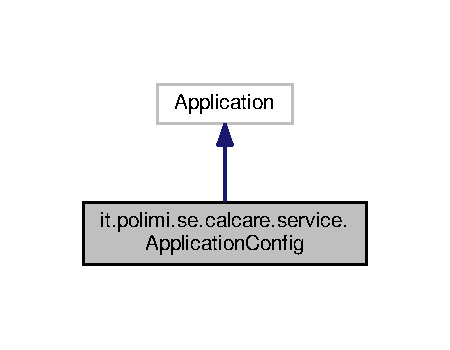
\includegraphics[width=216pt]{classit_1_1polimi_1_1se_1_1calcare_1_1service_1_1ApplicationConfig__inherit__graph}
\end{center}
\end{figure}


Collaboration diagram for it.\+polimi.\+se.\+calcare.\+service.\+Application\+Config\+:
\nopagebreak
\begin{figure}[H]
\begin{center}
\leavevmode
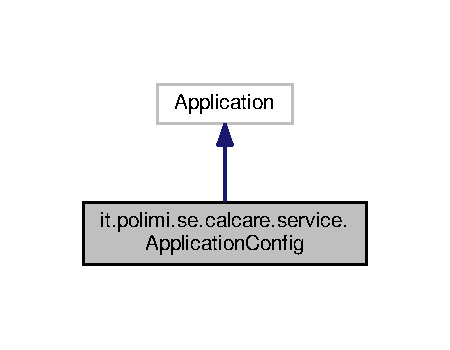
\includegraphics[width=216pt]{classit_1_1polimi_1_1se_1_1calcare_1_1service_1_1ApplicationConfig__coll__graph}
\end{center}
\end{figure}
\subsection*{Public Member Functions}
\begin{DoxyCompactItemize}
\item 
\hypertarget{classit_1_1polimi_1_1se_1_1calcare_1_1service_1_1ApplicationConfig_a67890a3a721a56b4172cb7d9f0be94cd}{}Set$<$ Class$<$?$>$ $>$ {\bfseries get\+Classes} ()\label{classit_1_1polimi_1_1se_1_1calcare_1_1service_1_1ApplicationConfig_a67890a3a721a56b4172cb7d9f0be94cd}

\end{DoxyCompactItemize}


\subsection{Detailed Description}
\begin{DoxyAuthor}{Author}
tyrion 
\end{DoxyAuthor}


The documentation for this class was generated from the following file\+:\begin{DoxyCompactItemize}
\item 
src/main/java/it/polimi/se/calcare/service/Application\+Config.\+java\end{DoxyCompactItemize}

\hypertarget{classit_1_1polimi_1_1se_1_1calcare_1_1auth_1_1AuthFilter}{}\section{it.\+polimi.\+se.\+calcare.\+auth.\+Auth\+Filter Class Reference}
\label{classit_1_1polimi_1_1se_1_1calcare_1_1auth_1_1AuthFilter}\index{it.\+polimi.\+se.\+calcare.\+auth.\+Auth\+Filter@{it.\+polimi.\+se.\+calcare.\+auth.\+Auth\+Filter}}


Inheritance diagram for it.\+polimi.\+se.\+calcare.\+auth.\+Auth\+Filter\+:
\nopagebreak
\begin{figure}[H]
\begin{center}
\leavevmode
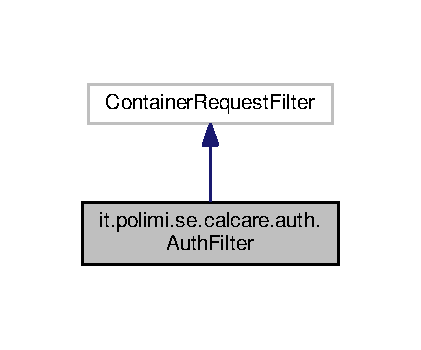
\includegraphics[width=202pt]{classit_1_1polimi_1_1se_1_1calcare_1_1auth_1_1AuthFilter__inherit__graph}
\end{center}
\end{figure}


Collaboration diagram for it.\+polimi.\+se.\+calcare.\+auth.\+Auth\+Filter\+:
\nopagebreak
\begin{figure}[H]
\begin{center}
\leavevmode
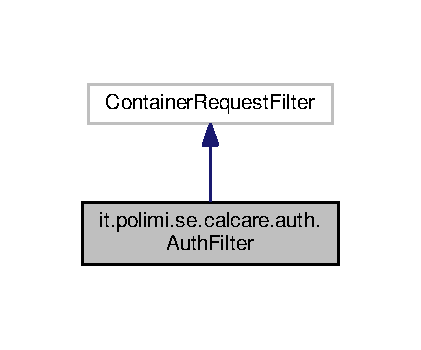
\includegraphics[width=202pt]{classit_1_1polimi_1_1se_1_1calcare_1_1auth_1_1AuthFilter__coll__graph}
\end{center}
\end{figure}
\subsection*{Public Member Functions}
\begin{DoxyCompactItemize}
\item 
\hypertarget{classit_1_1polimi_1_1se_1_1calcare_1_1auth_1_1AuthFilter_a9666e2671c62689caaa306a18ceb47f0}{}void {\bfseries filter} (Container\+Request\+Context request\+Context)  throws I\+O\+Exception \label{classit_1_1polimi_1_1se_1_1calcare_1_1auth_1_1AuthFilter_a9666e2671c62689caaa306a18ceb47f0}

\end{DoxyCompactItemize}


\subsection{Detailed Description}
\begin{DoxyAuthor}{Author}
Germano Gabbianelli 
\end{DoxyAuthor}


The documentation for this class was generated from the following file\+:\begin{DoxyCompactItemize}
\item 
src/main/java/it/polimi/se/calcare/auth/Auth\+Filter.\+java\end{DoxyCompactItemize}

\hypertarget{interfaceit_1_1polimi_1_1se_1_1calcare_1_1auth_1_1AuthRequired}{}\section{it.\+polimi.\+se.\+calcare.\+auth.\+Auth\+Required Interface Reference}
\label{interfaceit_1_1polimi_1_1se_1_1calcare_1_1auth_1_1AuthRequired}\index{it.\+polimi.\+se.\+calcare.\+auth.\+Auth\+Required@{it.\+polimi.\+se.\+calcare.\+auth.\+Auth\+Required}}


\subsection{Detailed Description}
\begin{DoxyAuthor}{Author}
tyrion 
\end{DoxyAuthor}


The documentation for this interface was generated from the following file\+:\begin{DoxyCompactItemize}
\item 
src/main/java/it/polimi/se/calcare/auth/Auth\+Required.\+java\end{DoxyCompactItemize}

\hypertarget{classit_1_1polimi_1_1se_1_1calcare_1_1service_1_1AuthREST}{}\section{it.\+polimi.\+se.\+calcare.\+service.\+Auth\+R\+E\+S\+T Class Reference}
\label{classit_1_1polimi_1_1se_1_1calcare_1_1service_1_1AuthREST}\index{it.\+polimi.\+se.\+calcare.\+service.\+Auth\+R\+E\+S\+T@{it.\+polimi.\+se.\+calcare.\+service.\+Auth\+R\+E\+S\+T}}
\subsection*{Public Member Functions}
\begin{DoxyCompactItemize}
\item 
\hypertarget{classit_1_1polimi_1_1se_1_1calcare_1_1service_1_1AuthREST_a36709d01a316a13d00e992883e990c3d}{}String {\bfseries login} (@Form\+Param(\char`\"{}email\char`\"{}) String email,@Form\+Param(\char`\"{}password\char`\"{}) String password)  throws Invalid\+Key\+Spec\+Exception, No\+Such\+Algorithm\+Exception \label{classit_1_1polimi_1_1se_1_1calcare_1_1service_1_1AuthREST_a36709d01a316a13d00e992883e990c3d}

\item 
\hypertarget{classit_1_1polimi_1_1se_1_1calcare_1_1service_1_1AuthREST_a05920ad51ca1056ea0784f2406a53391}{}Response {\bfseries activate} (@Query\+Param(\char`\"{}token\char`\"{}) String token)  throws U\+R\+I\+Syntax\+Exception \label{classit_1_1polimi_1_1se_1_1calcare_1_1service_1_1AuthREST_a05920ad51ca1056ea0784f2406a53391}

\item 
\hypertarget{classit_1_1polimi_1_1se_1_1calcare_1_1service_1_1AuthREST_a0f04c50820dc3f1ecdddc9ca1d452b0d}{}void {\bfseries request\+Reset} (@Context Uri\+Info ui,@Form\+Param(\char`\"{}email\char`\"{}) String email)\label{classit_1_1polimi_1_1se_1_1calcare_1_1service_1_1AuthREST_a0f04c50820dc3f1ecdddc9ca1d452b0d}

\item 
\hypertarget{classit_1_1polimi_1_1se_1_1calcare_1_1service_1_1AuthREST_a794517d0b58b85de51c18ce17f44f9bd}{}void {\bfseries reset} (@Query\+Param(\char`\"{}token\char`\"{}) String token,@Form\+Param(\char`\"{}password\char`\"{}) String password)  throws No\+Such\+Algorithm\+Exception, Invalid\+Key\+Spec\+Exception \label{classit_1_1polimi_1_1se_1_1calcare_1_1service_1_1AuthREST_a794517d0b58b85de51c18ce17f44f9bd}

\end{DoxyCompactItemize}


\subsection{Detailed Description}
\begin{DoxyAuthor}{Author}
Germano Gabbianelli 
\end{DoxyAuthor}


The documentation for this class was generated from the following file\+:\begin{DoxyCompactItemize}
\item 
src/main/java/it/polimi/se/calcare/service/Auth\+R\+E\+S\+T.\+java\end{DoxyCompactItemize}

\hypertarget{classit_1_1polimi_1_1se_1_1calcare_1_1entities_1_1Calendar}{}\section{it.\+polimi.\+se.\+calcare.\+entities.\+Calendar Class Reference}
\label{classit_1_1polimi_1_1se_1_1calcare_1_1entities_1_1Calendar}\index{it.\+polimi.\+se.\+calcare.\+entities.\+Calendar@{it.\+polimi.\+se.\+calcare.\+entities.\+Calendar}}


Inheritance diagram for it.\+polimi.\+se.\+calcare.\+entities.\+Calendar\+:
\nopagebreak
\begin{figure}[H]
\begin{center}
\leavevmode
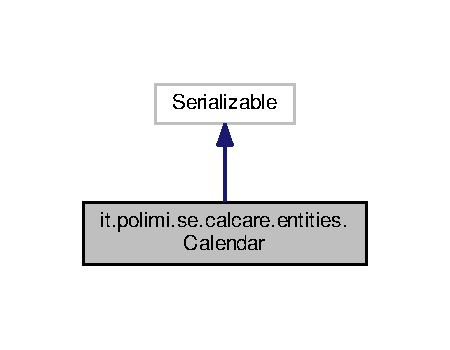
\includegraphics[width=216pt]{classit_1_1polimi_1_1se_1_1calcare_1_1entities_1_1Calendar__inherit__graph}
\end{center}
\end{figure}


Collaboration diagram for it.\+polimi.\+se.\+calcare.\+entities.\+Calendar\+:
\nopagebreak
\begin{figure}[H]
\begin{center}
\leavevmode
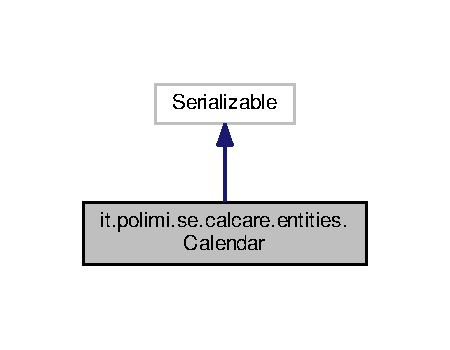
\includegraphics[width=216pt]{classit_1_1polimi_1_1se_1_1calcare_1_1entities_1_1Calendar__coll__graph}
\end{center}
\end{figure}
\subsection*{Public Member Functions}
\begin{DoxyCompactItemize}
\item 
\hypertarget{classit_1_1polimi_1_1se_1_1calcare_1_1entities_1_1Calendar_a4b694cd9a0d7edbfacaf27d05eafce25}{}{\bfseries Calendar} (Integer id)\label{classit_1_1polimi_1_1se_1_1calcare_1_1entities_1_1Calendar_a4b694cd9a0d7edbfacaf27d05eafce25}

\item 
\hypertarget{classit_1_1polimi_1_1se_1_1calcare_1_1entities_1_1Calendar_abe4ad69a4d27afdbd007c742c5b3d322}{}Integer {\bfseries get\+Id} ()\label{classit_1_1polimi_1_1se_1_1calcare_1_1entities_1_1Calendar_abe4ad69a4d27afdbd007c742c5b3d322}

\item 
\hypertarget{classit_1_1polimi_1_1se_1_1calcare_1_1entities_1_1Calendar_af3c8ffef24b326ef527295b712b467e1}{}void {\bfseries set\+Id} (Integer id)\label{classit_1_1polimi_1_1se_1_1calcare_1_1entities_1_1Calendar_af3c8ffef24b326ef527295b712b467e1}

\item 
\hypertarget{classit_1_1polimi_1_1se_1_1calcare_1_1entities_1_1Calendar_ace37d2f5c23bd063a513d48cd5847aea}{}Collection$<$ \hyperlink{classit_1_1polimi_1_1se_1_1calcare_1_1entities_1_1Participation}{Participation} $>$ {\bfseries get\+Participations} ()\label{classit_1_1polimi_1_1se_1_1calcare_1_1entities_1_1Calendar_ace37d2f5c23bd063a513d48cd5847aea}

\item 
\hypertarget{classit_1_1polimi_1_1se_1_1calcare_1_1entities_1_1Calendar_a914f950fec30819fa9686b42b8dd80c6}{}void {\bfseries set\+Participations} (Collection$<$ \hyperlink{classit_1_1polimi_1_1se_1_1calcare_1_1entities_1_1Participation}{Participation} $>$ participations)\label{classit_1_1polimi_1_1se_1_1calcare_1_1entities_1_1Calendar_a914f950fec30819fa9686b42b8dd80c6}

\item 
\hypertarget{classit_1_1polimi_1_1se_1_1calcare_1_1entities_1_1Calendar_ac3553a3082f38c57773530d40a17da52}{}\hyperlink{classit_1_1polimi_1_1se_1_1calcare_1_1entities_1_1User}{User} {\bfseries get\+Owner} ()\label{classit_1_1polimi_1_1se_1_1calcare_1_1entities_1_1Calendar_ac3553a3082f38c57773530d40a17da52}

\item 
\hypertarget{classit_1_1polimi_1_1se_1_1calcare_1_1entities_1_1Calendar_a43182f5983ed119449e483a5630681fd}{}void {\bfseries set\+Owner} (\hyperlink{classit_1_1polimi_1_1se_1_1calcare_1_1entities_1_1User}{User} owner)\label{classit_1_1polimi_1_1se_1_1calcare_1_1entities_1_1Calendar_a43182f5983ed119449e483a5630681fd}

\item 
\hypertarget{classit_1_1polimi_1_1se_1_1calcare_1_1entities_1_1Calendar_a3805c9ee047f832b106388fb3a31e4af}{}boolean {\bfseries is\+Public1} ()\label{classit_1_1polimi_1_1se_1_1calcare_1_1entities_1_1Calendar_a3805c9ee047f832b106388fb3a31e4af}

\item 
\hypertarget{classit_1_1polimi_1_1se_1_1calcare_1_1entities_1_1Calendar_a55c70c2a35e885e2d38ebe1fab062bb4}{}void {\bfseries set\+Public1} (boolean public1)\label{classit_1_1polimi_1_1se_1_1calcare_1_1entities_1_1Calendar_a55c70c2a35e885e2d38ebe1fab062bb4}

\item 
\hypertarget{classit_1_1polimi_1_1se_1_1calcare_1_1entities_1_1Calendar_a655824cdc3f1895f015870aa962b54bc}{}int {\bfseries hash\+Code} ()\label{classit_1_1polimi_1_1se_1_1calcare_1_1entities_1_1Calendar_a655824cdc3f1895f015870aa962b54bc}

\item 
\hypertarget{classit_1_1polimi_1_1se_1_1calcare_1_1entities_1_1Calendar_a64bb62df3fc9a5cd6bcc8db8afbbd1b4}{}boolean {\bfseries equals} (Object object)\label{classit_1_1polimi_1_1se_1_1calcare_1_1entities_1_1Calendar_a64bb62df3fc9a5cd6bcc8db8afbbd1b4}

\item 
\hypertarget{classit_1_1polimi_1_1se_1_1calcare_1_1entities_1_1Calendar_a262e85f6dcb926ca360d0e5c2d9c266c}{}String {\bfseries to\+String} ()\label{classit_1_1polimi_1_1se_1_1calcare_1_1entities_1_1Calendar_a262e85f6dcb926ca360d0e5c2d9c266c}

\end{DoxyCompactItemize}


\subsection{Detailed Description}
\begin{DoxyAuthor}{Author}
tyrion 
\end{DoxyAuthor}


The documentation for this class was generated from the following file\+:\begin{DoxyCompactItemize}
\item 
src/main/java/it/polimi/se/calcare/entities/Calendar.\+java\end{DoxyCompactItemize}

\hypertarget{classit_1_1polimi_1_1se_1_1calcare_1_1service_1_1CalendarFacadeREST}{}\section{it.\+polimi.\+se.\+calcare.\+service.\+Calendar\+Facade\+R\+E\+S\+T Class Reference}
\label{classit_1_1polimi_1_1se_1_1calcare_1_1service_1_1CalendarFacadeREST}\index{it.\+polimi.\+se.\+calcare.\+service.\+Calendar\+Facade\+R\+E\+S\+T@{it.\+polimi.\+se.\+calcare.\+service.\+Calendar\+Facade\+R\+E\+S\+T}}


Inheritance diagram for it.\+polimi.\+se.\+calcare.\+service.\+Calendar\+Facade\+R\+E\+S\+T\+:
\nopagebreak
\begin{figure}[H]
\begin{center}
\leavevmode
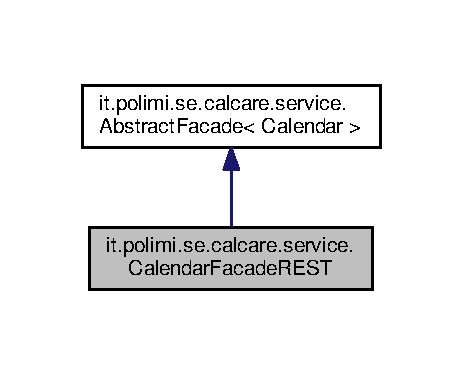
\includegraphics[width=222pt]{classit_1_1polimi_1_1se_1_1calcare_1_1service_1_1CalendarFacadeREST__inherit__graph}
\end{center}
\end{figure}


Collaboration diagram for it.\+polimi.\+se.\+calcare.\+service.\+Calendar\+Facade\+R\+E\+S\+T\+:
\nopagebreak
\begin{figure}[H]
\begin{center}
\leavevmode
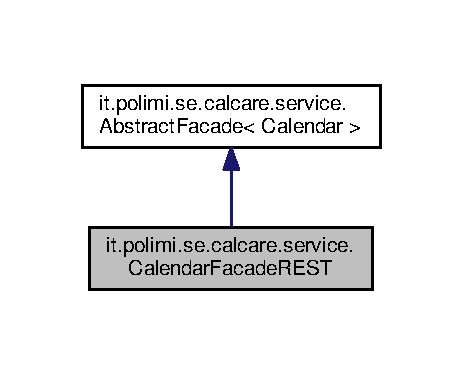
\includegraphics[width=222pt]{classit_1_1polimi_1_1se_1_1calcare_1_1service_1_1CalendarFacadeREST__coll__graph}
\end{center}
\end{figure}
\subsection*{Public Member Functions}
\begin{DoxyCompactItemize}
\item 
\hypertarget{classit_1_1polimi_1_1se_1_1calcare_1_1service_1_1CalendarFacadeREST_a04bdd0182e21e1b351b927dfa35c2e30}{}void {\bfseries edit} (@Context Security\+Context sc, \hyperlink{classit_1_1polimi_1_1se_1_1calcare_1_1entities_1_1Calendar}{Calendar} entity)\label{classit_1_1polimi_1_1se_1_1calcare_1_1service_1_1CalendarFacadeREST_a04bdd0182e21e1b351b927dfa35c2e30}

\item 
\hypertarget{classit_1_1polimi_1_1se_1_1calcare_1_1service_1_1CalendarFacadeREST_abfd3b712872cd9402dd11f45c90f46d1}{}Set$<$ \hyperlink{classit_1_1polimi_1_1se_1_1calcare_1_1entities_1_1Event}{Event} $>$ {\bfseries find} (@Context Security\+Context sc,@Path\+Param(\char`\"{}id\char`\"{}) Integer id)\label{classit_1_1polimi_1_1se_1_1calcare_1_1service_1_1CalendarFacadeREST_abfd3b712872cd9402dd11f45c90f46d1}

\item 
\hypertarget{classit_1_1polimi_1_1se_1_1calcare_1_1service_1_1CalendarFacadeREST_a68d20ca828aba8fc2e6bec66366b7589}{}\hyperlink{classit_1_1polimi_1_1se_1_1calcare_1_1entities_1_1Calendar}{Calendar} {\bfseries my\+Calendar} (@Context Security\+Context sc)\label{classit_1_1polimi_1_1se_1_1calcare_1_1service_1_1CalendarFacadeREST_a68d20ca828aba8fc2e6bec66366b7589}

\item 
\hypertarget{classit_1_1polimi_1_1se_1_1calcare_1_1service_1_1CalendarFacadeREST_ac2e6ad5d570425d8ced1885b963f01df}{}List$<$ \hyperlink{classit_1_1polimi_1_1se_1_1calcare_1_1entities_1_1Event}{Event} $>$ {\bfseries my\+Events} (@Context Security\+Context sc)\label{classit_1_1polimi_1_1se_1_1calcare_1_1service_1_1CalendarFacadeREST_ac2e6ad5d570425d8ced1885b963f01df}

\item 
\hypertarget{classit_1_1polimi_1_1se_1_1calcare_1_1service_1_1CalendarFacadeREST_a9bc25eb65ea704a3db692a5c6a96fb13}{}List$<$ \hyperlink{classit_1_1polimi_1_1se_1_1calcare_1_1entities_1_1Calendar}{Calendar} $>$ {\bfseries search} (@Context Security\+Context sc,@Query\+Param(\char`\"{}search\char`\"{}) String search)\label{classit_1_1polimi_1_1se_1_1calcare_1_1service_1_1CalendarFacadeREST_a9bc25eb65ea704a3db692a5c6a96fb13}

\end{DoxyCompactItemize}
\subsection*{Protected Member Functions}
\begin{DoxyCompactItemize}
\item 
\hypertarget{classit_1_1polimi_1_1se_1_1calcare_1_1service_1_1CalendarFacadeREST_a7533056a006fadcb1fbd39a95efcde15}{}Entity\+Manager {\bfseries get\+Entity\+Manager} ()\label{classit_1_1polimi_1_1se_1_1calcare_1_1service_1_1CalendarFacadeREST_a7533056a006fadcb1fbd39a95efcde15}

\end{DoxyCompactItemize}


\subsection{Detailed Description}
\begin{DoxyAuthor}{Author}
tyrion 
\end{DoxyAuthor}


The documentation for this class was generated from the following file\+:\begin{DoxyCompactItemize}
\item 
src/main/java/it/polimi/se/calcare/service/Calendar\+Facade\+R\+E\+S\+T.\+java\end{DoxyCompactItemize}

\hypertarget{classit_1_1polimi_1_1se_1_1calcare_1_1entities_1_1City}{}\section{it.\+polimi.\+se.\+calcare.\+entities.\+City Class Reference}
\label{classit_1_1polimi_1_1se_1_1calcare_1_1entities_1_1City}\index{it.\+polimi.\+se.\+calcare.\+entities.\+City@{it.\+polimi.\+se.\+calcare.\+entities.\+City}}


Inheritance diagram for it.\+polimi.\+se.\+calcare.\+entities.\+City\+:
\nopagebreak
\begin{figure}[H]
\begin{center}
\leavevmode
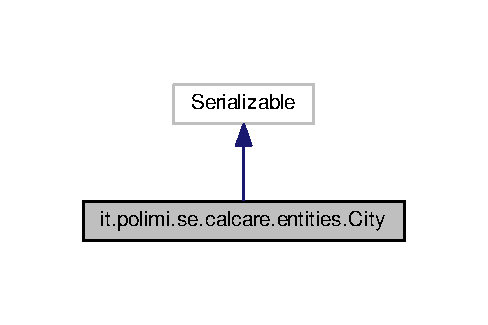
\includegraphics[width=234pt]{classit_1_1polimi_1_1se_1_1calcare_1_1entities_1_1City__inherit__graph}
\end{center}
\end{figure}


Collaboration diagram for it.\+polimi.\+se.\+calcare.\+entities.\+City\+:
\nopagebreak
\begin{figure}[H]
\begin{center}
\leavevmode
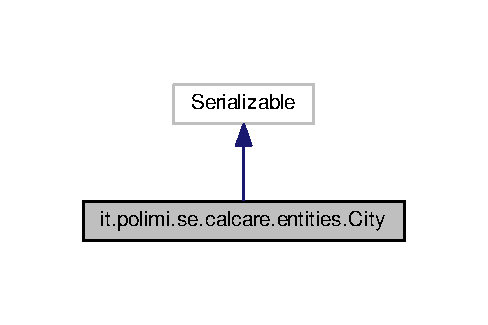
\includegraphics[width=234pt]{classit_1_1polimi_1_1se_1_1calcare_1_1entities_1_1City__coll__graph}
\end{center}
\end{figure}
\subsection*{Public Member Functions}
\begin{DoxyCompactItemize}
\item 
\hypertarget{classit_1_1polimi_1_1se_1_1calcare_1_1entities_1_1City_ac2566c554255c0e44cb9b590fac66372}{}{\bfseries City} (Integer id)\label{classit_1_1polimi_1_1se_1_1calcare_1_1entities_1_1City_ac2566c554255c0e44cb9b590fac66372}

\item 
\hypertarget{classit_1_1polimi_1_1se_1_1calcare_1_1entities_1_1City_a581d638ef5b6cd5b880cd6f1f8b2aae3}{}{\bfseries City} (Integer id, String name, String country, double lat, double lon)\label{classit_1_1polimi_1_1se_1_1calcare_1_1entities_1_1City_a581d638ef5b6cd5b880cd6f1f8b2aae3}

\item 
\hypertarget{classit_1_1polimi_1_1se_1_1calcare_1_1entities_1_1City_a77b168520fa5d9f79469350bd52cbb3b}{}Integer {\bfseries get\+Id} ()\label{classit_1_1polimi_1_1se_1_1calcare_1_1entities_1_1City_a77b168520fa5d9f79469350bd52cbb3b}

\item 
\hypertarget{classit_1_1polimi_1_1se_1_1calcare_1_1entities_1_1City_a116f4f546769fb27e6be4715fa38c12e}{}void {\bfseries set\+Id} (Integer id)\label{classit_1_1polimi_1_1se_1_1calcare_1_1entities_1_1City_a116f4f546769fb27e6be4715fa38c12e}

\item 
\hypertarget{classit_1_1polimi_1_1se_1_1calcare_1_1entities_1_1City_a15adea2517549737d2f6a7c6f65ac763}{}String {\bfseries get\+Name} ()\label{classit_1_1polimi_1_1se_1_1calcare_1_1entities_1_1City_a15adea2517549737d2f6a7c6f65ac763}

\item 
\hypertarget{classit_1_1polimi_1_1se_1_1calcare_1_1entities_1_1City_a205c0895a1a10b5c30421241eaab0a4e}{}void {\bfseries set\+Name} (String name)\label{classit_1_1polimi_1_1se_1_1calcare_1_1entities_1_1City_a205c0895a1a10b5c30421241eaab0a4e}

\item 
\hypertarget{classit_1_1polimi_1_1se_1_1calcare_1_1entities_1_1City_a2bd87b3c2f3b05e1a32711cd8a138764}{}String {\bfseries get\+Country} ()\label{classit_1_1polimi_1_1se_1_1calcare_1_1entities_1_1City_a2bd87b3c2f3b05e1a32711cd8a138764}

\item 
\hypertarget{classit_1_1polimi_1_1se_1_1calcare_1_1entities_1_1City_a065dd94b514f4c5c10fb30a9d9f68289}{}void {\bfseries set\+Country} (String country)\label{classit_1_1polimi_1_1se_1_1calcare_1_1entities_1_1City_a065dd94b514f4c5c10fb30a9d9f68289}

\item 
\hypertarget{classit_1_1polimi_1_1se_1_1calcare_1_1entities_1_1City_acab3320c22fe931ed7c635b2a91f1343}{}double {\bfseries get\+Lat} ()\label{classit_1_1polimi_1_1se_1_1calcare_1_1entities_1_1City_acab3320c22fe931ed7c635b2a91f1343}

\item 
\hypertarget{classit_1_1polimi_1_1se_1_1calcare_1_1entities_1_1City_abde80d0f3553f3e69296dbc33569d9d9}{}void {\bfseries set\+Lat} (double lat)\label{classit_1_1polimi_1_1se_1_1calcare_1_1entities_1_1City_abde80d0f3553f3e69296dbc33569d9d9}

\item 
\hypertarget{classit_1_1polimi_1_1se_1_1calcare_1_1entities_1_1City_a8cce50294f2989e2be3c9292c560f398}{}double {\bfseries get\+Lon} ()\label{classit_1_1polimi_1_1se_1_1calcare_1_1entities_1_1City_a8cce50294f2989e2be3c9292c560f398}

\item 
\hypertarget{classit_1_1polimi_1_1se_1_1calcare_1_1entities_1_1City_ab726f0f78830d23f7c9478e15733a46e}{}void {\bfseries set\+Lon} (double lon)\label{classit_1_1polimi_1_1se_1_1calcare_1_1entities_1_1City_ab726f0f78830d23f7c9478e15733a46e}

\item 
\hypertarget{classit_1_1polimi_1_1se_1_1calcare_1_1entities_1_1City_a2bf75f13fb13f7ec94516723b387435c}{}Collection$<$ \hyperlink{classit_1_1polimi_1_1se_1_1calcare_1_1entities_1_1Forecast}{Forecast} $>$ {\bfseries get\+Forecast\+Collection} ()\label{classit_1_1polimi_1_1se_1_1calcare_1_1entities_1_1City_a2bf75f13fb13f7ec94516723b387435c}

\item 
\hypertarget{classit_1_1polimi_1_1se_1_1calcare_1_1entities_1_1City_ab93b2bfc72713c390054c835c90c446b}{}void {\bfseries set\+Forecast\+Collection} (Collection$<$ \hyperlink{classit_1_1polimi_1_1se_1_1calcare_1_1entities_1_1Forecast}{Forecast} $>$ forecast\+Collection)\label{classit_1_1polimi_1_1se_1_1calcare_1_1entities_1_1City_ab93b2bfc72713c390054c835c90c446b}

\item 
\hypertarget{classit_1_1polimi_1_1se_1_1calcare_1_1entities_1_1City_a94005ca9288c08969fb5767a404cc416}{}int {\bfseries hash\+Code} ()\label{classit_1_1polimi_1_1se_1_1calcare_1_1entities_1_1City_a94005ca9288c08969fb5767a404cc416}

\item 
\hypertarget{classit_1_1polimi_1_1se_1_1calcare_1_1entities_1_1City_a5c94dd16479f63b97ba866ee25bac358}{}boolean {\bfseries equals} (Object object)\label{classit_1_1polimi_1_1se_1_1calcare_1_1entities_1_1City_a5c94dd16479f63b97ba866ee25bac358}

\item 
\hypertarget{classit_1_1polimi_1_1se_1_1calcare_1_1entities_1_1City_a278e1d7ba177eeca173d739ce6ea6087}{}String {\bfseries to\+String} ()\label{classit_1_1polimi_1_1se_1_1calcare_1_1entities_1_1City_a278e1d7ba177eeca173d739ce6ea6087}

\end{DoxyCompactItemize}


\subsection{Detailed Description}
\begin{DoxyAuthor}{Author}
tyrion 
\end{DoxyAuthor}


The documentation for this class was generated from the following file\+:\begin{DoxyCompactItemize}
\item 
src/main/java/it/polimi/se/calcare/entities/City.\+java\end{DoxyCompactItemize}

\hypertarget{classit_1_1polimi_1_1se_1_1calcare_1_1service_1_1CronJob}{}\section{it.\+polimi.\+se.\+calcare.\+service.\+Cron\+Job Class Reference}
\label{classit_1_1polimi_1_1se_1_1calcare_1_1service_1_1CronJob}\index{it.\+polimi.\+se.\+calcare.\+service.\+Cron\+Job@{it.\+polimi.\+se.\+calcare.\+service.\+Cron\+Job}}
\subsection*{Public Member Functions}
\begin{DoxyCompactItemize}
\item 
\hypertarget{classit_1_1polimi_1_1se_1_1calcare_1_1service_1_1CronJob_a22994d0fa211234bf11e8a0db5cd5bfe}{}void {\bfseries Weather\+Fetcher} ()  throws I\+O\+Exception, J\+S\+O\+N\+Exception, Exception \label{classit_1_1polimi_1_1se_1_1calcare_1_1service_1_1CronJob_a22994d0fa211234bf11e8a0db5cd5bfe}

\end{DoxyCompactItemize}


\subsection{Detailed Description}
\begin{DoxyAuthor}{Author}
nopesled 
\end{DoxyAuthor}


The documentation for this class was generated from the following file\+:\begin{DoxyCompactItemize}
\item 
src/main/java/it/polimi/se/calcare/service/Cron\+Job.\+java\end{DoxyCompactItemize}

\hypertarget{enumit_1_1polimi_1_1se_1_1calcare_1_1entities_1_1NotificationType_1_1Enum}{}\section{it.\+polimi.\+se.\+calcare.\+entities.\+Notification\+Type.\+Enum Enum Reference}
\label{enumit_1_1polimi_1_1se_1_1calcare_1_1entities_1_1NotificationType_1_1Enum}\index{it.\+polimi.\+se.\+calcare.\+entities.\+Notification\+Type.\+Enum@{it.\+polimi.\+se.\+calcare.\+entities.\+Notification\+Type.\+Enum}}
\subsection*{Public Member Functions}
\begin{DoxyCompactItemize}
\item 
\hypertarget{enumit_1_1polimi_1_1se_1_1calcare_1_1entities_1_1NotificationType_1_1Enum_ae1d9ef339458399ebe409ab70061709e}{}{\bfseries Enum} (int id)\label{enumit_1_1polimi_1_1se_1_1calcare_1_1entities_1_1NotificationType_1_1Enum_ae1d9ef339458399ebe409ab70061709e}

\end{DoxyCompactItemize}
\subsection*{Public Attributes}
\begin{DoxyCompactItemize}
\item 
\hypertarget{enumit_1_1polimi_1_1se_1_1calcare_1_1entities_1_1NotificationType_1_1Enum_a024e3ae1725b727ecec210fa3eef3b53}{}{\bfseries I\+N\+V\+I\+T\+A\+T\+I\+O\+N} =(1)\label{enumit_1_1polimi_1_1se_1_1calcare_1_1entities_1_1NotificationType_1_1Enum_a024e3ae1725b727ecec210fa3eef3b53}

\item 
\hypertarget{enumit_1_1polimi_1_1se_1_1calcare_1_1entities_1_1NotificationType_1_1Enum_aaa8ae588a5c0cd41cb0e2a6be0a82d03}{}{\bfseries B\+A\+D\+\_\+\+W\+E\+A\+T\+H\+E\+R} =(2)\label{enumit_1_1polimi_1_1se_1_1calcare_1_1entities_1_1NotificationType_1_1Enum_aaa8ae588a5c0cd41cb0e2a6be0a82d03}

\item 
\hypertarget{enumit_1_1polimi_1_1se_1_1calcare_1_1entities_1_1NotificationType_1_1Enum_ad0924c9dceea31e3ac66b0b01559093b}{}int {\bfseries id}\label{enumit_1_1polimi_1_1se_1_1calcare_1_1entities_1_1NotificationType_1_1Enum_ad0924c9dceea31e3ac66b0b01559093b}

\end{DoxyCompactItemize}


The documentation for this enum was generated from the following file\+:\begin{DoxyCompactItemize}
\item 
src/main/java/it/polimi/se/calcare/entities/Notification\+Type.\+java\end{DoxyCompactItemize}

\hypertarget{classit_1_1polimi_1_1se_1_1calcare_1_1entities_1_1Event}{}\section{it.\+polimi.\+se.\+calcare.\+entities.\+Event Class Reference}
\label{classit_1_1polimi_1_1se_1_1calcare_1_1entities_1_1Event}\index{it.\+polimi.\+se.\+calcare.\+entities.\+Event@{it.\+polimi.\+se.\+calcare.\+entities.\+Event}}


Inheritance diagram for it.\+polimi.\+se.\+calcare.\+entities.\+Event\+:
\nopagebreak
\begin{figure}[H]
\begin{center}
\leavevmode
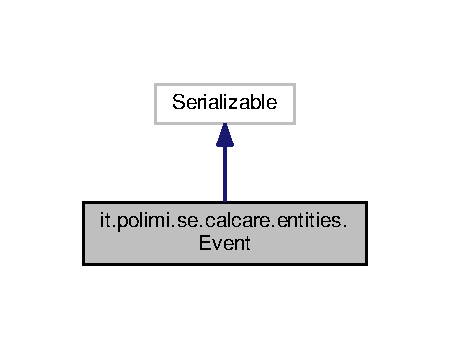
\includegraphics[width=216pt]{classit_1_1polimi_1_1se_1_1calcare_1_1entities_1_1Event__inherit__graph}
\end{center}
\end{figure}


Collaboration diagram for it.\+polimi.\+se.\+calcare.\+entities.\+Event\+:
\nopagebreak
\begin{figure}[H]
\begin{center}
\leavevmode
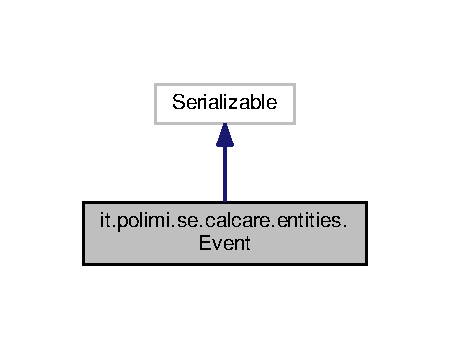
\includegraphics[width=216pt]{classit_1_1polimi_1_1se_1_1calcare_1_1entities_1_1Event__coll__graph}
\end{center}
\end{figure}
\subsection*{Public Member Functions}
\begin{DoxyCompactItemize}
\item 
\hypertarget{classit_1_1polimi_1_1se_1_1calcare_1_1entities_1_1Event_aa9dbce8fcd05bcea3761e66dc7db5170}{}{\bfseries Event} (Integer id)\label{classit_1_1polimi_1_1se_1_1calcare_1_1entities_1_1Event_aa9dbce8fcd05bcea3761e66dc7db5170}

\item 
\hypertarget{classit_1_1polimi_1_1se_1_1calcare_1_1entities_1_1Event_a952ea31c07198381750f4af6d1f78477}{}{\bfseries Event} (String name, String description, Date start, Date end, String location, boolean public1, boolean outdoor)\label{classit_1_1polimi_1_1se_1_1calcare_1_1entities_1_1Event_a952ea31c07198381750f4af6d1f78477}

\item 
\hypertarget{classit_1_1polimi_1_1se_1_1calcare_1_1entities_1_1Event_a8f9b6d4b4de5754c983f54b7769e640e}{}{\bfseries Event} (Date start, Date end, boolean public1)\label{classit_1_1polimi_1_1se_1_1calcare_1_1entities_1_1Event_a8f9b6d4b4de5754c983f54b7769e640e}

\item 
\hypertarget{classit_1_1polimi_1_1se_1_1calcare_1_1entities_1_1Event_a395d0695be24d71fa15af0e071443fbe}{}Integer {\bfseries get\+Id} ()\label{classit_1_1polimi_1_1se_1_1calcare_1_1entities_1_1Event_a395d0695be24d71fa15af0e071443fbe}

\item 
\hypertarget{classit_1_1polimi_1_1se_1_1calcare_1_1entities_1_1Event_a027d540dbb700956502abf436486950a}{}void {\bfseries set\+Id} (Integer id)\label{classit_1_1polimi_1_1se_1_1calcare_1_1entities_1_1Event_a027d540dbb700956502abf436486950a}

\item 
\hypertarget{classit_1_1polimi_1_1se_1_1calcare_1_1entities_1_1Event_a4392f7dbc87e48e97a2dcdeb6f3b911d}{}String {\bfseries get\+Name} ()\label{classit_1_1polimi_1_1se_1_1calcare_1_1entities_1_1Event_a4392f7dbc87e48e97a2dcdeb6f3b911d}

\item 
\hypertarget{classit_1_1polimi_1_1se_1_1calcare_1_1entities_1_1Event_a26d02455538160aca57a9399db6b7f11}{}void {\bfseries set\+Name} (String name)\label{classit_1_1polimi_1_1se_1_1calcare_1_1entities_1_1Event_a26d02455538160aca57a9399db6b7f11}

\item 
\hypertarget{classit_1_1polimi_1_1se_1_1calcare_1_1entities_1_1Event_a1145bbb5a44ef12dba67e064a4e0ee52}{}String {\bfseries get\+Description} ()\label{classit_1_1polimi_1_1se_1_1calcare_1_1entities_1_1Event_a1145bbb5a44ef12dba67e064a4e0ee52}

\item 
\hypertarget{classit_1_1polimi_1_1se_1_1calcare_1_1entities_1_1Event_a36086d5cf3746ef26c67be67a6b5c171}{}void {\bfseries set\+Description} (String description)\label{classit_1_1polimi_1_1se_1_1calcare_1_1entities_1_1Event_a36086d5cf3746ef26c67be67a6b5c171}

\item 
\hypertarget{classit_1_1polimi_1_1se_1_1calcare_1_1entities_1_1Event_ae723fe9d531a0a2c4900733cc2f67aaf}{}Date {\bfseries get\+Start} ()\label{classit_1_1polimi_1_1se_1_1calcare_1_1entities_1_1Event_ae723fe9d531a0a2c4900733cc2f67aaf}

\item 
\hypertarget{classit_1_1polimi_1_1se_1_1calcare_1_1entities_1_1Event_a06ff76ae5fd70ce2659ce2485d8faf5d}{}void {\bfseries set\+Start} (Date start)\label{classit_1_1polimi_1_1se_1_1calcare_1_1entities_1_1Event_a06ff76ae5fd70ce2659ce2485d8faf5d}

\item 
\hypertarget{classit_1_1polimi_1_1se_1_1calcare_1_1entities_1_1Event_aab23436c6fdae1391637d4b1c51d5067}{}Date {\bfseries get\+End} ()\label{classit_1_1polimi_1_1se_1_1calcare_1_1entities_1_1Event_aab23436c6fdae1391637d4b1c51d5067}

\item 
\hypertarget{classit_1_1polimi_1_1se_1_1calcare_1_1entities_1_1Event_a65218adfc913a1e2f375485bba714b9d}{}void {\bfseries set\+End} (Date end)\label{classit_1_1polimi_1_1se_1_1calcare_1_1entities_1_1Event_a65218adfc913a1e2f375485bba714b9d}

\item 
\hypertarget{classit_1_1polimi_1_1se_1_1calcare_1_1entities_1_1Event_ae6303a03bcf2a1deb2b445059b887c8a}{}String {\bfseries get\+Location} ()\label{classit_1_1polimi_1_1se_1_1calcare_1_1entities_1_1Event_ae6303a03bcf2a1deb2b445059b887c8a}

\item 
\hypertarget{classit_1_1polimi_1_1se_1_1calcare_1_1entities_1_1Event_aa5d868bb1201cc4194be82449988a79c}{}void {\bfseries set\+Location} (String location)\label{classit_1_1polimi_1_1se_1_1calcare_1_1entities_1_1Event_aa5d868bb1201cc4194be82449988a79c}

\item 
\hypertarget{classit_1_1polimi_1_1se_1_1calcare_1_1entities_1_1Event_a191f6f43eb65f1e6fb7d4a7a675cd7a5}{}boolean {\bfseries get\+Public1} ()\label{classit_1_1polimi_1_1se_1_1calcare_1_1entities_1_1Event_a191f6f43eb65f1e6fb7d4a7a675cd7a5}

\item 
\hypertarget{classit_1_1polimi_1_1se_1_1calcare_1_1entities_1_1Event_a840285afcc62db4966463a1027376eb9}{}boolean {\bfseries is\+Public} ()\label{classit_1_1polimi_1_1se_1_1calcare_1_1entities_1_1Event_a840285afcc62db4966463a1027376eb9}

\item 
\hypertarget{classit_1_1polimi_1_1se_1_1calcare_1_1entities_1_1Event_ab28a4a23e0b81f12f2f0bd3b97d24fb4}{}void {\bfseries set\+Public1} (boolean public1)\label{classit_1_1polimi_1_1se_1_1calcare_1_1entities_1_1Event_ab28a4a23e0b81f12f2f0bd3b97d24fb4}

\item 
\hypertarget{classit_1_1polimi_1_1se_1_1calcare_1_1entities_1_1Event_a473bbf5dbff7ab837740a94ec4ad6310}{}boolean {\bfseries get\+Outdoor} ()\label{classit_1_1polimi_1_1se_1_1calcare_1_1entities_1_1Event_a473bbf5dbff7ab837740a94ec4ad6310}

\item 
\hypertarget{classit_1_1polimi_1_1se_1_1calcare_1_1entities_1_1Event_a0821ab0a8d25f512ab8e8c65e8927464}{}void {\bfseries set\+Outdoor} (boolean outdoor)\label{classit_1_1polimi_1_1se_1_1calcare_1_1entities_1_1Event_a0821ab0a8d25f512ab8e8c65e8927464}

\item 
\hypertarget{classit_1_1polimi_1_1se_1_1calcare_1_1entities_1_1Event_a8176fb114557edb00a588d87219af9f7}{}Collection$<$ \hyperlink{classit_1_1polimi_1_1se_1_1calcare_1_1entities_1_1Forecast}{Forecast} $>$ {\bfseries get\+Forecast\+Collection} ()\label{classit_1_1polimi_1_1se_1_1calcare_1_1entities_1_1Event_a8176fb114557edb00a588d87219af9f7}

\item 
\hypertarget{classit_1_1polimi_1_1se_1_1calcare_1_1entities_1_1Event_a45d9c15f902214d8e22836ae0e13532a}{}void {\bfseries set\+Forecast\+Collection} (Collection$<$ \hyperlink{classit_1_1polimi_1_1se_1_1calcare_1_1entities_1_1Forecast}{Forecast} $>$ forecast\+Collection)\label{classit_1_1polimi_1_1se_1_1calcare_1_1entities_1_1Event_a45d9c15f902214d8e22836ae0e13532a}

\item 
\hypertarget{classit_1_1polimi_1_1se_1_1calcare_1_1entities_1_1Event_ad1de0661e729b64833e72e7509ced8df}{}Collection$<$ \hyperlink{classit_1_1polimi_1_1se_1_1calcare_1_1entities_1_1Participation}{Participation} $>$ {\bfseries get\+Participation\+Collection} ()\label{classit_1_1polimi_1_1se_1_1calcare_1_1entities_1_1Event_ad1de0661e729b64833e72e7509ced8df}

\item 
\hypertarget{classit_1_1polimi_1_1se_1_1calcare_1_1entities_1_1Event_a2d0da7776532a7554a9ef9272456732a}{}void {\bfseries set\+Participation\+Collection} (Collection$<$ \hyperlink{classit_1_1polimi_1_1se_1_1calcare_1_1entities_1_1Participation}{Participation} $>$ participation\+Collection)\label{classit_1_1polimi_1_1se_1_1calcare_1_1entities_1_1Event_a2d0da7776532a7554a9ef9272456732a}

\item 
\hypertarget{classit_1_1polimi_1_1se_1_1calcare_1_1entities_1_1Event_a4ae9f2f663e4e4b3a91b5e6a1c20c141}{}\hyperlink{classit_1_1polimi_1_1se_1_1calcare_1_1entities_1_1User}{User} {\bfseries get\+Creator} ()\label{classit_1_1polimi_1_1se_1_1calcare_1_1entities_1_1Event_a4ae9f2f663e4e4b3a91b5e6a1c20c141}

\item 
\hypertarget{classit_1_1polimi_1_1se_1_1calcare_1_1entities_1_1Event_a91d1e805ad4e851669a3ff232da7c689}{}void {\bfseries set\+Creator} (\hyperlink{classit_1_1polimi_1_1se_1_1calcare_1_1entities_1_1User}{User} creator)\label{classit_1_1polimi_1_1se_1_1calcare_1_1entities_1_1Event_a91d1e805ad4e851669a3ff232da7c689}

\item 
\hypertarget{classit_1_1polimi_1_1se_1_1calcare_1_1entities_1_1Event_af356746cd7178b8bf143c29cbf361208}{}Collection$<$ \hyperlink{classit_1_1polimi_1_1se_1_1calcare_1_1entities_1_1Notification}{Notification} $>$ {\bfseries get\+Notification\+Collection} ()\label{classit_1_1polimi_1_1se_1_1calcare_1_1entities_1_1Event_af356746cd7178b8bf143c29cbf361208}

\item 
\hypertarget{classit_1_1polimi_1_1se_1_1calcare_1_1entities_1_1Event_a31d71e15c3830c9eee0afc0ee67b7472}{}void {\bfseries set\+Notification\+Collection} (Collection$<$ \hyperlink{classit_1_1polimi_1_1se_1_1calcare_1_1entities_1_1Notification}{Notification} $>$ notification\+Collection)\label{classit_1_1polimi_1_1se_1_1calcare_1_1entities_1_1Event_a31d71e15c3830c9eee0afc0ee67b7472}

\item 
\hypertarget{classit_1_1polimi_1_1se_1_1calcare_1_1entities_1_1Event_a992fa4b6cb5b007ed3b7930e77876efe}{}\hyperlink{classit_1_1polimi_1_1se_1_1calcare_1_1entities_1_1Event}{Event} {\bfseries as\+Private} ()\label{classit_1_1polimi_1_1se_1_1calcare_1_1entities_1_1Event_a992fa4b6cb5b007ed3b7930e77876efe}

\item 
\hypertarget{classit_1_1polimi_1_1se_1_1calcare_1_1entities_1_1Event_a99a35dcd572db1c9582c9e98903e31e4}{}int {\bfseries hash\+Code} ()\label{classit_1_1polimi_1_1se_1_1calcare_1_1entities_1_1Event_a99a35dcd572db1c9582c9e98903e31e4}

\item 
\hypertarget{classit_1_1polimi_1_1se_1_1calcare_1_1entities_1_1Event_a09a889e40e2cbc229f7551e1e7722c51}{}boolean {\bfseries equals} (Object object)\label{classit_1_1polimi_1_1se_1_1calcare_1_1entities_1_1Event_a09a889e40e2cbc229f7551e1e7722c51}

\item 
\hypertarget{classit_1_1polimi_1_1se_1_1calcare_1_1entities_1_1Event_a1a40c338f72de06feae2ccd1528f09e1}{}String {\bfseries to\+String} ()\label{classit_1_1polimi_1_1se_1_1calcare_1_1entities_1_1Event_a1a40c338f72de06feae2ccd1528f09e1}

\end{DoxyCompactItemize}


\subsection{Detailed Description}
\begin{DoxyAuthor}{Author}
tyrion 
\end{DoxyAuthor}


The documentation for this class was generated from the following file\+:\begin{DoxyCompactItemize}
\item 
src/main/java/it/polimi/se/calcare/entities/Event.\+java\end{DoxyCompactItemize}

\hypertarget{classit_1_1polimi_1_1se_1_1calcare_1_1dto_1_1EventCreationDTO}{}\section{it.\+polimi.\+se.\+calcare.\+dto.\+Event\+Creation\+D\+T\+O Class Reference}
\label{classit_1_1polimi_1_1se_1_1calcare_1_1dto_1_1EventCreationDTO}\index{it.\+polimi.\+se.\+calcare.\+dto.\+Event\+Creation\+D\+T\+O@{it.\+polimi.\+se.\+calcare.\+dto.\+Event\+Creation\+D\+T\+O}}


Collaboration diagram for it.\+polimi.\+se.\+calcare.\+dto.\+Event\+Creation\+D\+T\+O\+:
\nopagebreak
\begin{figure}[H]
\begin{center}
\leavevmode
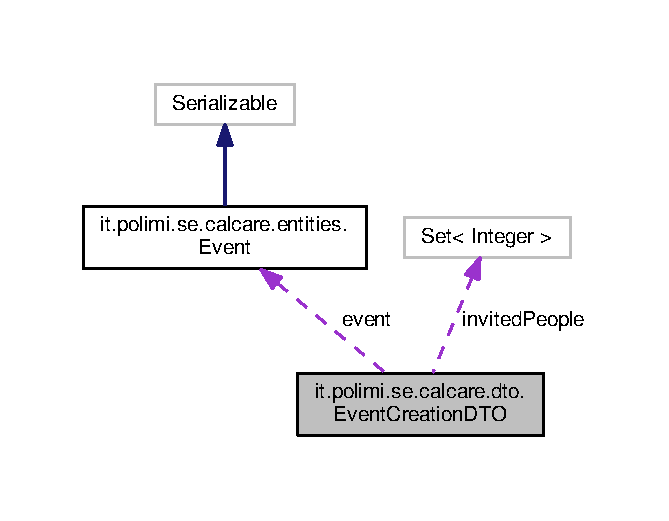
\includegraphics[width=321pt]{classit_1_1polimi_1_1se_1_1calcare_1_1dto_1_1EventCreationDTO__coll__graph}
\end{center}
\end{figure}
\subsection*{Public Member Functions}
\begin{DoxyCompactItemize}
\item 
\hypertarget{classit_1_1polimi_1_1se_1_1calcare_1_1dto_1_1EventCreationDTO_a7ee4324875e336c23f075caf06561751}{}{\bfseries Event\+Creation\+D\+T\+O} (\hyperlink{classit_1_1polimi_1_1se_1_1calcare_1_1entities_1_1Event}{Event} event, Set$<$ Integer $>$ invited\+Users)\label{classit_1_1polimi_1_1se_1_1calcare_1_1dto_1_1EventCreationDTO_a7ee4324875e336c23f075caf06561751}

\item 
\hypertarget{classit_1_1polimi_1_1se_1_1calcare_1_1dto_1_1EventCreationDTO_a6f3bcda113265f8c4a3071ffb2977681}{}\hyperlink{classit_1_1polimi_1_1se_1_1calcare_1_1entities_1_1Event}{Event} {\bfseries get\+Event} ()\label{classit_1_1polimi_1_1se_1_1calcare_1_1dto_1_1EventCreationDTO_a6f3bcda113265f8c4a3071ffb2977681}

\item 
\hypertarget{classit_1_1polimi_1_1se_1_1calcare_1_1dto_1_1EventCreationDTO_a6ae3b65ab0857992db099ee89820f0ca}{}void {\bfseries set\+Event} (\hyperlink{classit_1_1polimi_1_1se_1_1calcare_1_1entities_1_1Event}{Event} event)\label{classit_1_1polimi_1_1se_1_1calcare_1_1dto_1_1EventCreationDTO_a6ae3b65ab0857992db099ee89820f0ca}

\item 
\hypertarget{classit_1_1polimi_1_1se_1_1calcare_1_1dto_1_1EventCreationDTO_ad9b1f369ad67162a728aa3a9ccd38ea0}{}Set$<$ Integer $>$ {\bfseries get\+Invited\+People} ()\label{classit_1_1polimi_1_1se_1_1calcare_1_1dto_1_1EventCreationDTO_ad9b1f369ad67162a728aa3a9ccd38ea0}

\item 
\hypertarget{classit_1_1polimi_1_1se_1_1calcare_1_1dto_1_1EventCreationDTO_a91571aa5f0ab2bd3caa347f4bf3b3e14}{}void {\bfseries set\+Invited\+People} (Set$<$ Integer $>$ invitations)\label{classit_1_1polimi_1_1se_1_1calcare_1_1dto_1_1EventCreationDTO_a91571aa5f0ab2bd3caa347f4bf3b3e14}

\end{DoxyCompactItemize}
\subsection*{Public Attributes}
\begin{DoxyCompactItemize}
\item 
\hypertarget{classit_1_1polimi_1_1se_1_1calcare_1_1dto_1_1EventCreationDTO_a50823f0fc4a3afa12df71e7cd91d869c}{}Set$<$ Integer $>$ {\bfseries invited\+People}\label{classit_1_1polimi_1_1se_1_1calcare_1_1dto_1_1EventCreationDTO_a50823f0fc4a3afa12df71e7cd91d869c}

\item 
\hypertarget{classit_1_1polimi_1_1se_1_1calcare_1_1dto_1_1EventCreationDTO_a1e255633cbfbde8acae6c22a11bb4eea}{}\hyperlink{classit_1_1polimi_1_1se_1_1calcare_1_1entities_1_1Event}{Event} {\bfseries event}\label{classit_1_1polimi_1_1se_1_1calcare_1_1dto_1_1EventCreationDTO_a1e255633cbfbde8acae6c22a11bb4eea}

\end{DoxyCompactItemize}


\subsection{Detailed Description}
\begin{DoxyAuthor}{Author}
tyrion 
\end{DoxyAuthor}


The documentation for this class was generated from the following file\+:\begin{DoxyCompactItemize}
\item 
src/main/java/it/polimi/se/calcare/dto/Event\+Creation\+D\+T\+O.\+java\end{DoxyCompactItemize}

\hypertarget{classit_1_1polimi_1_1se_1_1calcare_1_1service_1_1EventFacadeREST}{}\section{it.\+polimi.\+se.\+calcare.\+service.\+Event\+Facade\+R\+E\+S\+T Class Reference}
\label{classit_1_1polimi_1_1se_1_1calcare_1_1service_1_1EventFacadeREST}\index{it.\+polimi.\+se.\+calcare.\+service.\+Event\+Facade\+R\+E\+S\+T@{it.\+polimi.\+se.\+calcare.\+service.\+Event\+Facade\+R\+E\+S\+T}}


Inheritance diagram for it.\+polimi.\+se.\+calcare.\+service.\+Event\+Facade\+R\+E\+S\+T\+:
\nopagebreak
\begin{figure}[H]
\begin{center}
\leavevmode
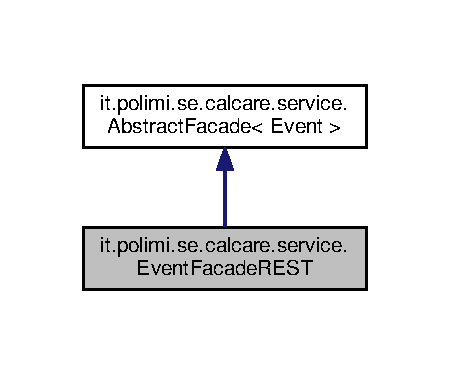
\includegraphics[width=216pt]{classit_1_1polimi_1_1se_1_1calcare_1_1service_1_1EventFacadeREST__inherit__graph}
\end{center}
\end{figure}


Collaboration diagram for it.\+polimi.\+se.\+calcare.\+service.\+Event\+Facade\+R\+E\+S\+T\+:
\nopagebreak
\begin{figure}[H]
\begin{center}
\leavevmode
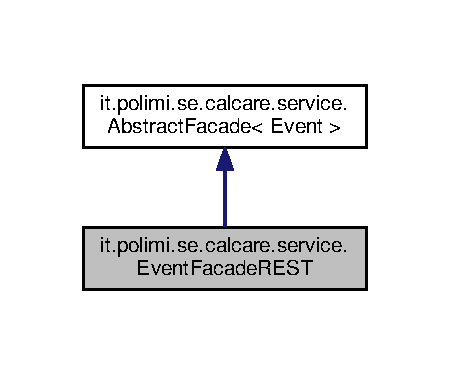
\includegraphics[width=216pt]{classit_1_1polimi_1_1se_1_1calcare_1_1service_1_1EventFacadeREST__coll__graph}
\end{center}
\end{figure}
\subsection*{Public Member Functions}
\begin{DoxyCompactItemize}
\item 
\hypertarget{classit_1_1polimi_1_1se_1_1calcare_1_1service_1_1EventFacadeREST_acc0b1abeab2fbf12f94180b4effda96a}{}void {\bfseries create} (@Context Security\+Context sc,@Context Uri\+Info ui, \hyperlink{classit_1_1polimi_1_1se_1_1calcare_1_1dto_1_1EventCreationDTO}{Event\+Creation\+D\+T\+O} dto)\label{classit_1_1polimi_1_1se_1_1calcare_1_1service_1_1EventFacadeREST_acc0b1abeab2fbf12f94180b4effda96a}

\item 
\hypertarget{classit_1_1polimi_1_1se_1_1calcare_1_1service_1_1EventFacadeREST_adabd62722187873ca23b5689165bafb0}{}void {\bfseries edit} (@Context Security\+Context sc,@Context Uri\+Info ui,@Path\+Param(\char`\"{}id\char`\"{}) Integer id, \hyperlink{classit_1_1polimi_1_1se_1_1calcare_1_1dto_1_1EventCreationDTO}{Event\+Creation\+D\+T\+O} dto)\label{classit_1_1polimi_1_1se_1_1calcare_1_1service_1_1EventFacadeREST_adabd62722187873ca23b5689165bafb0}

\item 
\hypertarget{classit_1_1polimi_1_1se_1_1calcare_1_1service_1_1EventFacadeREST_a1e2228b3dd8b8f1fcdf32f246502941c}{}void {\bfseries remove} (@Context Security\+Context sc,@Path\+Param(\char`\"{}id\char`\"{}) Integer id)\label{classit_1_1polimi_1_1se_1_1calcare_1_1service_1_1EventFacadeREST_a1e2228b3dd8b8f1fcdf32f246502941c}

\item 
\hypertarget{classit_1_1polimi_1_1se_1_1calcare_1_1service_1_1EventFacadeREST_a23370b711d4e6afaf3525f236a08cf49}{}\hyperlink{classit_1_1polimi_1_1se_1_1calcare_1_1entities_1_1Event}{Event} {\bfseries find} (@Context Security\+Context sc,@Path\+Param(\char`\"{}id\char`\"{}) Integer id)\label{classit_1_1polimi_1_1se_1_1calcare_1_1service_1_1EventFacadeREST_a23370b711d4e6afaf3525f236a08cf49}

\end{DoxyCompactItemize}
\subsection*{Protected Member Functions}
\begin{DoxyCompactItemize}
\item 
\hypertarget{classit_1_1polimi_1_1se_1_1calcare_1_1service_1_1EventFacadeREST_ac000259f01de3a74f6e0dc418d7fcae4}{}Entity\+Manager {\bfseries get\+Entity\+Manager} ()\label{classit_1_1polimi_1_1se_1_1calcare_1_1service_1_1EventFacadeREST_ac000259f01de3a74f6e0dc418d7fcae4}

\end{DoxyCompactItemize}


\subsection{Detailed Description}
\begin{DoxyAuthor}{Author}
tyrion 
\end{DoxyAuthor}


The documentation for this class was generated from the following file\+:\begin{DoxyCompactItemize}
\item 
src/main/java/it/polimi/se/calcare/service/Event\+Facade\+R\+E\+S\+T.\+java\end{DoxyCompactItemize}

\hypertarget{classit_1_1polimi_1_1se_1_1calcare_1_1entities_1_1Forecast}{}\section{it.\+polimi.\+se.\+calcare.\+entities.\+Forecast Class Reference}
\label{classit_1_1polimi_1_1se_1_1calcare_1_1entities_1_1Forecast}\index{it.\+polimi.\+se.\+calcare.\+entities.\+Forecast@{it.\+polimi.\+se.\+calcare.\+entities.\+Forecast}}


Inheritance diagram for it.\+polimi.\+se.\+calcare.\+entities.\+Forecast\+:
\nopagebreak
\begin{figure}[H]
\begin{center}
\leavevmode
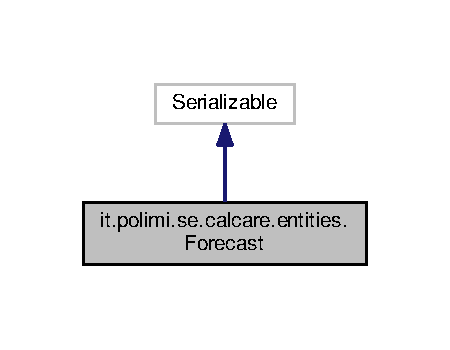
\includegraphics[width=216pt]{classit_1_1polimi_1_1se_1_1calcare_1_1entities_1_1Forecast__inherit__graph}
\end{center}
\end{figure}


Collaboration diagram for it.\+polimi.\+se.\+calcare.\+entities.\+Forecast\+:
\nopagebreak
\begin{figure}[H]
\begin{center}
\leavevmode
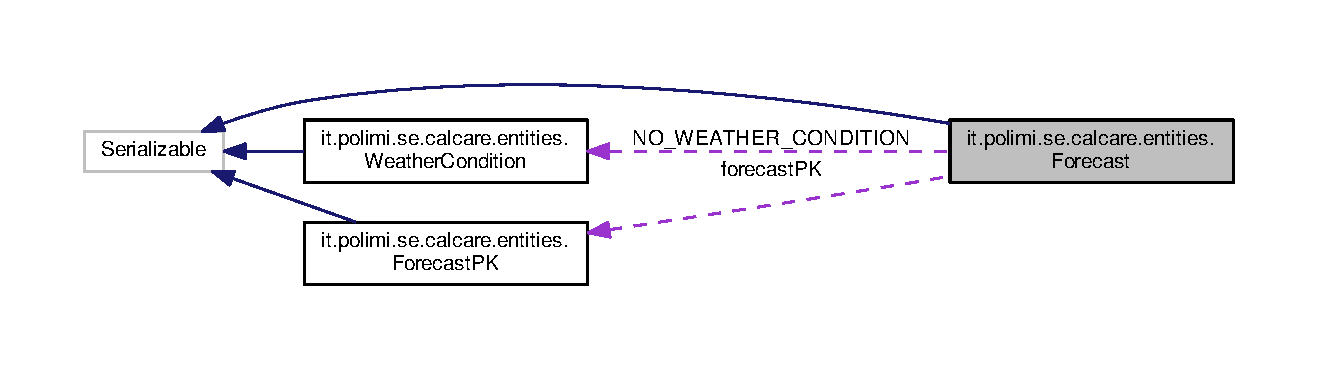
\includegraphics[width=350pt]{classit_1_1polimi_1_1se_1_1calcare_1_1entities_1_1Forecast__coll__graph}
\end{center}
\end{figure}
\subsection*{Public Member Functions}
\begin{DoxyCompactItemize}
\item 
\hypertarget{classit_1_1polimi_1_1se_1_1calcare_1_1entities_1_1Forecast_a9374b07d11df110bfe7376069217aed0}{}{\bfseries Forecast} (\hyperlink{classit_1_1polimi_1_1se_1_1calcare_1_1entities_1_1ForecastPK}{Forecast\+P\+K} forecast\+P\+K)\label{classit_1_1polimi_1_1se_1_1calcare_1_1entities_1_1Forecast_a9374b07d11df110bfe7376069217aed0}

\item 
\hypertarget{classit_1_1polimi_1_1se_1_1calcare_1_1entities_1_1Forecast_aed435f4ab688311e516a532595f33bc1}{}{\bfseries Forecast} (\hyperlink{classit_1_1polimi_1_1se_1_1calcare_1_1entities_1_1ForecastPK}{Forecast\+P\+K} forecast\+P\+K, double temp\+Min, double temp\+Max, double pressure, double humidity)\label{classit_1_1polimi_1_1se_1_1calcare_1_1entities_1_1Forecast_aed435f4ab688311e516a532595f33bc1}

\item 
\hypertarget{classit_1_1polimi_1_1se_1_1calcare_1_1entities_1_1Forecast_a14ba5435d7bf1ed8b770649911da7b76}{}{\bfseries Forecast} (Date dt, int city)\label{classit_1_1polimi_1_1se_1_1calcare_1_1entities_1_1Forecast_a14ba5435d7bf1ed8b770649911da7b76}

\item 
\hypertarget{classit_1_1polimi_1_1se_1_1calcare_1_1entities_1_1Forecast_a4523ab646ac8b0684abb5427fa4521e9}{}\hyperlink{classit_1_1polimi_1_1se_1_1calcare_1_1entities_1_1ForecastPK}{Forecast\+P\+K} {\bfseries get\+Forecast\+P\+K} ()\label{classit_1_1polimi_1_1se_1_1calcare_1_1entities_1_1Forecast_a4523ab646ac8b0684abb5427fa4521e9}

\item 
\hypertarget{classit_1_1polimi_1_1se_1_1calcare_1_1entities_1_1Forecast_a3646c4b684d5ef0f13108325eda98819}{}void {\bfseries set\+Forecast\+P\+K} (\hyperlink{classit_1_1polimi_1_1se_1_1calcare_1_1entities_1_1ForecastPK}{Forecast\+P\+K} forecast\+P\+K)\label{classit_1_1polimi_1_1se_1_1calcare_1_1entities_1_1Forecast_a3646c4b684d5ef0f13108325eda98819}

\item 
\hypertarget{classit_1_1polimi_1_1se_1_1calcare_1_1entities_1_1Forecast_ab3908583bf2bf774d6b346cf244533b1}{}double {\bfseries get\+Temp\+Min} ()\label{classit_1_1polimi_1_1se_1_1calcare_1_1entities_1_1Forecast_ab3908583bf2bf774d6b346cf244533b1}

\item 
\hypertarget{classit_1_1polimi_1_1se_1_1calcare_1_1entities_1_1Forecast_ab2c9021dca8686bcc0abfe3a46dd1543}{}void {\bfseries set\+Temp\+Min} (double temp\+Min)\label{classit_1_1polimi_1_1se_1_1calcare_1_1entities_1_1Forecast_ab2c9021dca8686bcc0abfe3a46dd1543}

\item 
\hypertarget{classit_1_1polimi_1_1se_1_1calcare_1_1entities_1_1Forecast_a95e33ba4e72a9f065b0ec9bc5a35d70c}{}double {\bfseries get\+Temp\+Max} ()\label{classit_1_1polimi_1_1se_1_1calcare_1_1entities_1_1Forecast_a95e33ba4e72a9f065b0ec9bc5a35d70c}

\item 
\hypertarget{classit_1_1polimi_1_1se_1_1calcare_1_1entities_1_1Forecast_abe6dffcc081ed97109e69cc8ce4b738d}{}void {\bfseries set\+Temp\+Max} (double temp\+Max)\label{classit_1_1polimi_1_1se_1_1calcare_1_1entities_1_1Forecast_abe6dffcc081ed97109e69cc8ce4b738d}

\item 
\hypertarget{classit_1_1polimi_1_1se_1_1calcare_1_1entities_1_1Forecast_ac4e598af4f6a0d9dd1eebddd43ddc9f1}{}double {\bfseries get\+Pressure} ()\label{classit_1_1polimi_1_1se_1_1calcare_1_1entities_1_1Forecast_ac4e598af4f6a0d9dd1eebddd43ddc9f1}

\item 
\hypertarget{classit_1_1polimi_1_1se_1_1calcare_1_1entities_1_1Forecast_a334c1d3184970b661fde27d822af6896}{}void {\bfseries set\+Pressure} (double pressure)\label{classit_1_1polimi_1_1se_1_1calcare_1_1entities_1_1Forecast_a334c1d3184970b661fde27d822af6896}

\item 
\hypertarget{classit_1_1polimi_1_1se_1_1calcare_1_1entities_1_1Forecast_a1bbbfde90c577657986b1b9344147f72}{}double {\bfseries get\+Humidity} ()\label{classit_1_1polimi_1_1se_1_1calcare_1_1entities_1_1Forecast_a1bbbfde90c577657986b1b9344147f72}

\item 
\hypertarget{classit_1_1polimi_1_1se_1_1calcare_1_1entities_1_1Forecast_a6b5d22246f239648729a3267bd748ecc}{}void {\bfseries set\+Humidity} (double humidity)\label{classit_1_1polimi_1_1se_1_1calcare_1_1entities_1_1Forecast_a6b5d22246f239648729a3267bd748ecc}

\item 
\hypertarget{classit_1_1polimi_1_1se_1_1calcare_1_1entities_1_1Forecast_abde4aa5f05fd64c1b2f22661add73963}{}Collection$<$ \hyperlink{classit_1_1polimi_1_1se_1_1calcare_1_1entities_1_1Event}{Event} $>$ {\bfseries get\+Event\+Collection} ()\label{classit_1_1polimi_1_1se_1_1calcare_1_1entities_1_1Forecast_abde4aa5f05fd64c1b2f22661add73963}

\item 
\hypertarget{classit_1_1polimi_1_1se_1_1calcare_1_1entities_1_1Forecast_afb5a603cbefc3fa67af3993cb25a9e5c}{}void {\bfseries set\+Event\+Collection} (Collection$<$ \hyperlink{classit_1_1polimi_1_1se_1_1calcare_1_1entities_1_1Event}{Event} $>$ event\+Collection)\label{classit_1_1polimi_1_1se_1_1calcare_1_1entities_1_1Forecast_afb5a603cbefc3fa67af3993cb25a9e5c}

\item 
\hypertarget{classit_1_1polimi_1_1se_1_1calcare_1_1entities_1_1Forecast_ab21758dce500fadd7be5767be33f3485}{}\hyperlink{classit_1_1polimi_1_1se_1_1calcare_1_1entities_1_1City}{City} {\bfseries get\+City1} ()\label{classit_1_1polimi_1_1se_1_1calcare_1_1entities_1_1Forecast_ab21758dce500fadd7be5767be33f3485}

\item 
\hypertarget{classit_1_1polimi_1_1se_1_1calcare_1_1entities_1_1Forecast_a89a40602154bda4e2e17faf8c65f7ce1}{}void {\bfseries set\+City1} (\hyperlink{classit_1_1polimi_1_1se_1_1calcare_1_1entities_1_1City}{City} city1)\label{classit_1_1polimi_1_1se_1_1calcare_1_1entities_1_1Forecast_a89a40602154bda4e2e17faf8c65f7ce1}

\item 
\hypertarget{classit_1_1polimi_1_1se_1_1calcare_1_1entities_1_1Forecast_a8a6123afb6d5fc1b98b0b7dcd9edd4ed}{}\hyperlink{classit_1_1polimi_1_1se_1_1calcare_1_1entities_1_1WeatherCondition}{Weather\+Condition} {\bfseries get\+Weather\+Condition} ()\label{classit_1_1polimi_1_1se_1_1calcare_1_1entities_1_1Forecast_a8a6123afb6d5fc1b98b0b7dcd9edd4ed}

\item 
\hypertarget{classit_1_1polimi_1_1se_1_1calcare_1_1entities_1_1Forecast_ab557545b6befbe2cbdefce0ab47aec8d}{}void {\bfseries set\+Weather\+Condition} (\hyperlink{classit_1_1polimi_1_1se_1_1calcare_1_1entities_1_1WeatherCondition}{Weather\+Condition} weather\+Condition)\label{classit_1_1polimi_1_1se_1_1calcare_1_1entities_1_1Forecast_ab557545b6befbe2cbdefce0ab47aec8d}

\item 
\hypertarget{classit_1_1polimi_1_1se_1_1calcare_1_1entities_1_1Forecast_a63f467375cfc1ee0432920c3810ee49a}{}int {\bfseries hash\+Code} ()\label{classit_1_1polimi_1_1se_1_1calcare_1_1entities_1_1Forecast_a63f467375cfc1ee0432920c3810ee49a}

\item 
\hypertarget{classit_1_1polimi_1_1se_1_1calcare_1_1entities_1_1Forecast_ae58197996ca50b8be377d34a044b8ab6}{}boolean {\bfseries equals} (Object object)\label{classit_1_1polimi_1_1se_1_1calcare_1_1entities_1_1Forecast_ae58197996ca50b8be377d34a044b8ab6}

\item 
\hypertarget{classit_1_1polimi_1_1se_1_1calcare_1_1entities_1_1Forecast_ad088566c059250844b4005298c9e0969}{}String {\bfseries to\+String} ()\label{classit_1_1polimi_1_1se_1_1calcare_1_1entities_1_1Forecast_ad088566c059250844b4005298c9e0969}

\end{DoxyCompactItemize}
\subsection*{Static Public Attributes}
\begin{DoxyCompactItemize}
\item 
\hypertarget{classit_1_1polimi_1_1se_1_1calcare_1_1entities_1_1Forecast_a000b56ea1b46fcd780c8410bc3fd2340}{}static final \hyperlink{classit_1_1polimi_1_1se_1_1calcare_1_1entities_1_1WeatherCondition}{Weather\+Condition} {\bfseries N\+O\+\_\+\+W\+E\+A\+T\+H\+E\+R\+\_\+\+C\+O\+N\+D\+I\+T\+I\+O\+N} = new \hyperlink{classit_1_1polimi_1_1se_1_1calcare_1_1entities_1_1WeatherCondition}{Weather\+Condition}(1)\label{classit_1_1polimi_1_1se_1_1calcare_1_1entities_1_1Forecast_a000b56ea1b46fcd780c8410bc3fd2340}

\end{DoxyCompactItemize}
\subsection*{Protected Attributes}
\begin{DoxyCompactItemize}
\item 
\hypertarget{classit_1_1polimi_1_1se_1_1calcare_1_1entities_1_1Forecast_ac5ae3b96d754a90aadd818afe9709898}{}\hyperlink{classit_1_1polimi_1_1se_1_1calcare_1_1entities_1_1ForecastPK}{Forecast\+P\+K} {\bfseries forecast\+P\+K}\label{classit_1_1polimi_1_1se_1_1calcare_1_1entities_1_1Forecast_ac5ae3b96d754a90aadd818afe9709898}

\end{DoxyCompactItemize}


\subsection{Detailed Description}
\begin{DoxyAuthor}{Author}
tyrion 
\end{DoxyAuthor}


The documentation for this class was generated from the following file\+:\begin{DoxyCompactItemize}
\item 
src/main/java/it/polimi/se/calcare/entities/Forecast.\+java\end{DoxyCompactItemize}

\hypertarget{classit_1_1polimi_1_1se_1_1calcare_1_1service_1_1ForecastFacadeREST}{}\section{it.\+polimi.\+se.\+calcare.\+service.\+Forecast\+Facade\+R\+E\+S\+T Class Reference}
\label{classit_1_1polimi_1_1se_1_1calcare_1_1service_1_1ForecastFacadeREST}\index{it.\+polimi.\+se.\+calcare.\+service.\+Forecast\+Facade\+R\+E\+S\+T@{it.\+polimi.\+se.\+calcare.\+service.\+Forecast\+Facade\+R\+E\+S\+T}}


Inheritance diagram for it.\+polimi.\+se.\+calcare.\+service.\+Forecast\+Facade\+R\+E\+S\+T\+:
\nopagebreak
\begin{figure}[H]
\begin{center}
\leavevmode
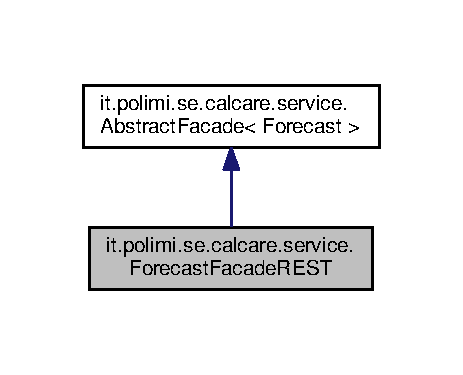
\includegraphics[width=222pt]{classit_1_1polimi_1_1se_1_1calcare_1_1service_1_1ForecastFacadeREST__inherit__graph}
\end{center}
\end{figure}


Collaboration diagram for it.\+polimi.\+se.\+calcare.\+service.\+Forecast\+Facade\+R\+E\+S\+T\+:
\nopagebreak
\begin{figure}[H]
\begin{center}
\leavevmode
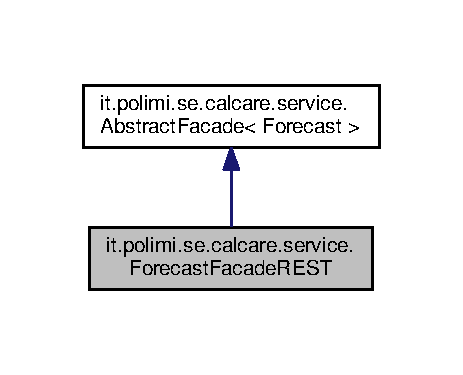
\includegraphics[width=222pt]{classit_1_1polimi_1_1se_1_1calcare_1_1service_1_1ForecastFacadeREST__coll__graph}
\end{center}
\end{figure}
\subsection*{Public Member Functions}
\begin{DoxyCompactItemize}
\item 
\hypertarget{classit_1_1polimi_1_1se_1_1calcare_1_1service_1_1ForecastFacadeREST_a54896d5e6334198568a173f5059b19d6}{}void {\bfseries create} (\hyperlink{classit_1_1polimi_1_1se_1_1calcare_1_1entities_1_1Forecast}{Forecast} entity)\label{classit_1_1polimi_1_1se_1_1calcare_1_1service_1_1ForecastFacadeREST_a54896d5e6334198568a173f5059b19d6}

\item 
\hypertarget{classit_1_1polimi_1_1se_1_1calcare_1_1service_1_1ForecastFacadeREST_a372ff8118fa18ef50053accf99863328}{}void {\bfseries edit} (@Path\+Param(\char`\"{}id\char`\"{}) Path\+Segment id, \hyperlink{classit_1_1polimi_1_1se_1_1calcare_1_1entities_1_1Forecast}{Forecast} entity)\label{classit_1_1polimi_1_1se_1_1calcare_1_1service_1_1ForecastFacadeREST_a372ff8118fa18ef50053accf99863328}

\item 
\hypertarget{classit_1_1polimi_1_1se_1_1calcare_1_1service_1_1ForecastFacadeREST_a66628ab23e5f3acecd3e814d533f31e0}{}void {\bfseries remove} (@Path\+Param(\char`\"{}id\char`\"{}) Path\+Segment id)\label{classit_1_1polimi_1_1se_1_1calcare_1_1service_1_1ForecastFacadeREST_a66628ab23e5f3acecd3e814d533f31e0}

\item 
\hypertarget{classit_1_1polimi_1_1se_1_1calcare_1_1service_1_1ForecastFacadeREST_a954a7bcc1ee93c9c611b0a34e2c09832}{}\hyperlink{classit_1_1polimi_1_1se_1_1calcare_1_1entities_1_1Forecast}{Forecast} {\bfseries find} (@Path\+Param(\char`\"{}id\char`\"{}) Path\+Segment id)\label{classit_1_1polimi_1_1se_1_1calcare_1_1service_1_1ForecastFacadeREST_a954a7bcc1ee93c9c611b0a34e2c09832}

\item 
\hypertarget{classit_1_1polimi_1_1se_1_1calcare_1_1service_1_1ForecastFacadeREST_ac2fa736e17085cff9edb801c9368ef0b}{}List$<$ \hyperlink{classit_1_1polimi_1_1se_1_1calcare_1_1entities_1_1Forecast}{Forecast} $>$ {\bfseries find\+All} ()\label{classit_1_1polimi_1_1se_1_1calcare_1_1service_1_1ForecastFacadeREST_ac2fa736e17085cff9edb801c9368ef0b}

\item 
\hypertarget{classit_1_1polimi_1_1se_1_1calcare_1_1service_1_1ForecastFacadeREST_a65569b25c9ad14af5599318b36097ac1}{}List$<$ \hyperlink{classit_1_1polimi_1_1se_1_1calcare_1_1entities_1_1Forecast}{Forecast} $>$ {\bfseries find\+Range} (@Path\+Param(\char`\"{}from\char`\"{}) Integer from,@Path\+Param(\char`\"{}to\char`\"{}) Integer to)\label{classit_1_1polimi_1_1se_1_1calcare_1_1service_1_1ForecastFacadeREST_a65569b25c9ad14af5599318b36097ac1}

\item 
\hypertarget{classit_1_1polimi_1_1se_1_1calcare_1_1service_1_1ForecastFacadeREST_afd00b4b31b45758d44b4426c895bdf7d}{}String {\bfseries count\+R\+E\+S\+T} ()\label{classit_1_1polimi_1_1se_1_1calcare_1_1service_1_1ForecastFacadeREST_afd00b4b31b45758d44b4426c895bdf7d}

\end{DoxyCompactItemize}
\subsection*{Protected Member Functions}
\begin{DoxyCompactItemize}
\item 
\hypertarget{classit_1_1polimi_1_1se_1_1calcare_1_1service_1_1ForecastFacadeREST_a54950bdac67672435d1c919ee939340c}{}Entity\+Manager {\bfseries get\+Entity\+Manager} ()\label{classit_1_1polimi_1_1se_1_1calcare_1_1service_1_1ForecastFacadeREST_a54950bdac67672435d1c919ee939340c}

\end{DoxyCompactItemize}


\subsection{Detailed Description}
\begin{DoxyAuthor}{Author}
tyrion 
\end{DoxyAuthor}


The documentation for this class was generated from the following file\+:\begin{DoxyCompactItemize}
\item 
src/main/java/it/polimi/se/calcare/service/Forecast\+Facade\+R\+E\+S\+T.\+java\end{DoxyCompactItemize}

\hypertarget{classit_1_1polimi_1_1se_1_1calcare_1_1entities_1_1ForecastPK}{}\section{it.\+polimi.\+se.\+calcare.\+entities.\+Forecast\+P\+K Class Reference}
\label{classit_1_1polimi_1_1se_1_1calcare_1_1entities_1_1ForecastPK}\index{it.\+polimi.\+se.\+calcare.\+entities.\+Forecast\+P\+K@{it.\+polimi.\+se.\+calcare.\+entities.\+Forecast\+P\+K}}


Inheritance diagram for it.\+polimi.\+se.\+calcare.\+entities.\+Forecast\+P\+K\+:
\nopagebreak
\begin{figure}[H]
\begin{center}
\leavevmode
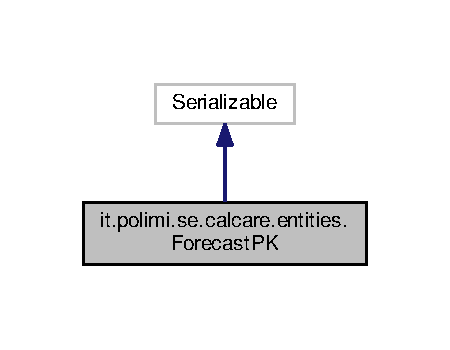
\includegraphics[width=216pt]{classit_1_1polimi_1_1se_1_1calcare_1_1entities_1_1ForecastPK__inherit__graph}
\end{center}
\end{figure}


Collaboration diagram for it.\+polimi.\+se.\+calcare.\+entities.\+Forecast\+P\+K\+:
\nopagebreak
\begin{figure}[H]
\begin{center}
\leavevmode
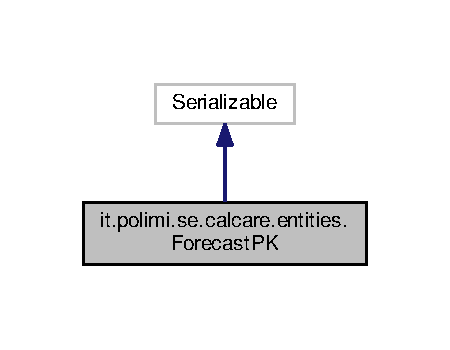
\includegraphics[width=216pt]{classit_1_1polimi_1_1se_1_1calcare_1_1entities_1_1ForecastPK__coll__graph}
\end{center}
\end{figure}
\subsection*{Public Member Functions}
\begin{DoxyCompactItemize}
\item 
\hypertarget{classit_1_1polimi_1_1se_1_1calcare_1_1entities_1_1ForecastPK_a050d123cc6b38ed08d34a62879bb53da}{}{\bfseries Forecast\+P\+K} (Date dt, int city)\label{classit_1_1polimi_1_1se_1_1calcare_1_1entities_1_1ForecastPK_a050d123cc6b38ed08d34a62879bb53da}

\item 
\hypertarget{classit_1_1polimi_1_1se_1_1calcare_1_1entities_1_1ForecastPK_a1096326f5838b5966fe0f48ca1223a43}{}Date {\bfseries get\+Dt} ()\label{classit_1_1polimi_1_1se_1_1calcare_1_1entities_1_1ForecastPK_a1096326f5838b5966fe0f48ca1223a43}

\item 
\hypertarget{classit_1_1polimi_1_1se_1_1calcare_1_1entities_1_1ForecastPK_ae566adf6bc589266d0344bdc3baa3606}{}void {\bfseries set\+Dt} (Date dt)\label{classit_1_1polimi_1_1se_1_1calcare_1_1entities_1_1ForecastPK_ae566adf6bc589266d0344bdc3baa3606}

\item 
\hypertarget{classit_1_1polimi_1_1se_1_1calcare_1_1entities_1_1ForecastPK_ac25b74d19708f1b16d53fd75066a9def}{}int {\bfseries get\+City} ()\label{classit_1_1polimi_1_1se_1_1calcare_1_1entities_1_1ForecastPK_ac25b74d19708f1b16d53fd75066a9def}

\item 
\hypertarget{classit_1_1polimi_1_1se_1_1calcare_1_1entities_1_1ForecastPK_abf4947d1cd4ec8ce2e9755d2a2f8d7e4}{}void {\bfseries set\+City} (int city)\label{classit_1_1polimi_1_1se_1_1calcare_1_1entities_1_1ForecastPK_abf4947d1cd4ec8ce2e9755d2a2f8d7e4}

\item 
\hypertarget{classit_1_1polimi_1_1se_1_1calcare_1_1entities_1_1ForecastPK_abc35136d5ad855baa5a2d9f9f5221cb7}{}int {\bfseries hash\+Code} ()\label{classit_1_1polimi_1_1se_1_1calcare_1_1entities_1_1ForecastPK_abc35136d5ad855baa5a2d9f9f5221cb7}

\item 
\hypertarget{classit_1_1polimi_1_1se_1_1calcare_1_1entities_1_1ForecastPK_a3dd52b73c2e725519bb502f4d593c837}{}boolean {\bfseries equals} (Object object)\label{classit_1_1polimi_1_1se_1_1calcare_1_1entities_1_1ForecastPK_a3dd52b73c2e725519bb502f4d593c837}

\item 
\hypertarget{classit_1_1polimi_1_1se_1_1calcare_1_1entities_1_1ForecastPK_a9d835a43e78a525964af95d4d86d25fd}{}String {\bfseries to\+String} ()\label{classit_1_1polimi_1_1se_1_1calcare_1_1entities_1_1ForecastPK_a9d835a43e78a525964af95d4d86d25fd}

\end{DoxyCompactItemize}


\subsection{Detailed Description}
\begin{DoxyAuthor}{Author}
tyrion 
\end{DoxyAuthor}


The documentation for this class was generated from the following file\+:\begin{DoxyCompactItemize}
\item 
src/main/java/it/polimi/se/calcare/entities/Forecast\+P\+K.\+java\end{DoxyCompactItemize}

\hypertarget{classit_1_1polimi_1_1se_1_1calcare_1_1service_1_1GetWeather}{}\section{it.\+polimi.\+se.\+calcare.\+service.\+Get\+Weather Class Reference}
\label{classit_1_1polimi_1_1se_1_1calcare_1_1service_1_1GetWeather}\index{it.\+polimi.\+se.\+calcare.\+service.\+Get\+Weather@{it.\+polimi.\+se.\+calcare.\+service.\+Get\+Weather}}
\subsection*{Public Member Functions}
\begin{DoxyCompactItemize}
\item 
\hypertarget{classit_1_1polimi_1_1se_1_1calcare_1_1service_1_1GetWeather_a8fbfe18f8715438086cc4cee3ba4680d}{}\hyperlink{classit_1_1polimi_1_1se_1_1calcare_1_1entities_1_1City}{City} {\bfseries create\+City} (String addr)  throws Malformed\+U\+R\+L\+Exception, I\+O\+Exception, J\+S\+O\+N\+Exception \label{classit_1_1polimi_1_1se_1_1calcare_1_1service_1_1GetWeather_a8fbfe18f8715438086cc4cee3ba4680d}

\item 
\hypertarget{classit_1_1polimi_1_1se_1_1calcare_1_1service_1_1GetWeather_ac1e81d436dd708ab46bdc7c92fce26b9}{}List$<$ \hyperlink{classit_1_1polimi_1_1se_1_1calcare_1_1entities_1_1Forecast}{Forecast} $>$ {\bfseries update\+Forecast} (\hyperlink{classit_1_1polimi_1_1se_1_1calcare_1_1entities_1_1City}{City} city, List$<$ \hyperlink{classit_1_1polimi_1_1se_1_1calcare_1_1entities_1_1Forecast}{Forecast} $>$ forecasts)  throws Malformed\+U\+R\+L\+Exception, J\+S\+O\+N\+Exception, I\+O\+Exception \label{classit_1_1polimi_1_1se_1_1calcare_1_1service_1_1GetWeather_ac1e81d436dd708ab46bdc7c92fce26b9}

\item 
\hypertarget{classit_1_1polimi_1_1se_1_1calcare_1_1service_1_1GetWeather_a4e1771ecd9db62feb3187696488edcb1}{}String {\bfseries json\+Builder} (Input\+Stream url\+Builder)\label{classit_1_1polimi_1_1se_1_1calcare_1_1service_1_1GetWeather_a4e1771ecd9db62feb3187696488edcb1}

\item 
\hypertarget{classit_1_1polimi_1_1se_1_1calcare_1_1service_1_1GetWeather_abf9661fb19282ffc9589e6bc1a9e8a26}{}void {\bfseries google\+Json\+Decoder} (J\+S\+O\+N\+Object obj, \hyperlink{classit_1_1polimi_1_1se_1_1calcare_1_1entities_1_1City}{City} new\+City)  throws J\+S\+O\+N\+Exception \label{classit_1_1polimi_1_1se_1_1calcare_1_1service_1_1GetWeather_abf9661fb19282ffc9589e6bc1a9e8a26}

\item 
\hypertarget{classit_1_1polimi_1_1se_1_1calcare_1_1service_1_1GetWeather_a1f45a4455bba9b3c50ac99279048c9bd}{}\hyperlink{classit_1_1polimi_1_1se_1_1calcare_1_1entities_1_1City}{City} {\bfseries openweather\+Json\+Decoder\+City} (J\+S\+O\+N\+Object obj, \hyperlink{classit_1_1polimi_1_1se_1_1calcare_1_1entities_1_1City}{City} new\+City)  throws J\+S\+O\+N\+Exception \label{classit_1_1polimi_1_1se_1_1calcare_1_1service_1_1GetWeather_a1f45a4455bba9b3c50ac99279048c9bd}

\item 
\hypertarget{classit_1_1polimi_1_1se_1_1calcare_1_1service_1_1GetWeather_a4a989fb5ee4c108ce4bf235637ea5169}{}\hyperlink{classit_1_1polimi_1_1se_1_1calcare_1_1entities_1_1Forecast}{Forecast} {\bfseries openweather\+Json\+Decoder\+Weather} (J\+S\+O\+N\+Object obj, \hyperlink{classit_1_1polimi_1_1se_1_1calcare_1_1entities_1_1Forecast}{Forecast} forecast, int day)  throws J\+S\+O\+N\+Exception \label{classit_1_1polimi_1_1se_1_1calcare_1_1service_1_1GetWeather_a4a989fb5ee4c108ce4bf235637ea5169}

\end{DoxyCompactItemize}
\subsection*{Static Public Member Functions}
\begin{DoxyCompactItemize}
\item 
\hypertarget{classit_1_1polimi_1_1se_1_1calcare_1_1service_1_1GetWeather_a89c2d71276ec050762a620f0a58c9c7d}{}static U\+R\+L {\bfseries google\+Url\+Builder} (String addr)  throws Malformed\+U\+R\+L\+Exception, Unsupported\+Encoding\+Exception \label{classit_1_1polimi_1_1se_1_1calcare_1_1service_1_1GetWeather_a89c2d71276ec050762a620f0a58c9c7d}

\item 
\hypertarget{classit_1_1polimi_1_1se_1_1calcare_1_1service_1_1GetWeather_a1f28fbf7200efedbac9fa5636629a3b8}{}static U\+R\+L {\bfseries open\+Weather\+Url\+Builder} (String addr)  throws Malformed\+U\+R\+L\+Exception, Unsupported\+Encoding\+Exception \label{classit_1_1polimi_1_1se_1_1calcare_1_1service_1_1GetWeather_a1f28fbf7200efedbac9fa5636629a3b8}

\end{DoxyCompactItemize}


\subsection{Detailed Description}
\begin{DoxyAuthor}{Author}
nopesled 
\end{DoxyAuthor}


The documentation for this class was generated from the following file\+:\begin{DoxyCompactItemize}
\item 
src/main/java/it/polimi/se/calcare/service/Get\+Weather.\+java\end{DoxyCompactItemize}

\hypertarget{classit_1_1polimi_1_1se_1_1calcare_1_1service_1_1GetWeatherTest}{}\section{it.\+polimi.\+se.\+calcare.\+service.\+Get\+Weather\+Test Class Reference}
\label{classit_1_1polimi_1_1se_1_1calcare_1_1service_1_1GetWeatherTest}\index{it.\+polimi.\+se.\+calcare.\+service.\+Get\+Weather\+Test@{it.\+polimi.\+se.\+calcare.\+service.\+Get\+Weather\+Test}}
\subsection*{Public Member Functions}
\begin{DoxyCompactItemize}
\item 
\hypertarget{classit_1_1polimi_1_1se_1_1calcare_1_1service_1_1GetWeatherTest_a82f8531eb5d015aedd627c6cc8eee188}{}void {\bfseries set\+Up} ()\label{classit_1_1polimi_1_1se_1_1calcare_1_1service_1_1GetWeatherTest_a82f8531eb5d015aedd627c6cc8eee188}

\item 
\hypertarget{classit_1_1polimi_1_1se_1_1calcare_1_1service_1_1GetWeatherTest_a9d16e1f7f237873a0a6f7b57702eee1d}{}void {\bfseries tear\+Down} ()\label{classit_1_1polimi_1_1se_1_1calcare_1_1service_1_1GetWeatherTest_a9d16e1f7f237873a0a6f7b57702eee1d}

\item 
\hypertarget{classit_1_1polimi_1_1se_1_1calcare_1_1service_1_1GetWeatherTest_a99d86fb1193ef9df8720dbb288058b01}{}void \hyperlink{classit_1_1polimi_1_1se_1_1calcare_1_1service_1_1GetWeatherTest_a99d86fb1193ef9df8720dbb288058b01}{test\+Google\+Url\+Builder} ()  throws Malformed\+U\+R\+L\+Exception, Unsupported\+Encoding\+Exception\label{classit_1_1polimi_1_1se_1_1calcare_1_1service_1_1GetWeatherTest_a99d86fb1193ef9df8720dbb288058b01}

\begin{DoxyCompactList}\small\item\em Test of google\+Url\+Builder method, of class \hyperlink{classit_1_1polimi_1_1se_1_1calcare_1_1service_1_1GetWeather}{Get\+Weather}. \end{DoxyCompactList}\item 
\hypertarget{classit_1_1polimi_1_1se_1_1calcare_1_1service_1_1GetWeatherTest_a33ceaf374463725008baf616ccffe54d}{}void \hyperlink{classit_1_1polimi_1_1se_1_1calcare_1_1service_1_1GetWeatherTest_a33ceaf374463725008baf616ccffe54d}{test\+Create\+City} ()  throws I\+O\+Exception, Malformed\+U\+R\+L\+Exception, J\+S\+O\+N\+Exception\label{classit_1_1polimi_1_1se_1_1calcare_1_1service_1_1GetWeatherTest_a33ceaf374463725008baf616ccffe54d}

\begin{DoxyCompactList}\small\item\em Test of create\+City method, of class \hyperlink{classit_1_1polimi_1_1se_1_1calcare_1_1service_1_1GetWeather}{Get\+Weather}. \end{DoxyCompactList}\item 
\hypertarget{classit_1_1polimi_1_1se_1_1calcare_1_1service_1_1GetWeatherTest_a0d504c7864bc0b0b5760327123a5bc66}{}void \hyperlink{classit_1_1polimi_1_1se_1_1calcare_1_1service_1_1GetWeatherTest_a0d504c7864bc0b0b5760327123a5bc66}{test\+Update\+Forecast} ()  throws J\+S\+O\+N\+Exception, I\+O\+Exception \label{classit_1_1polimi_1_1se_1_1calcare_1_1service_1_1GetWeatherTest_a0d504c7864bc0b0b5760327123a5bc66}

\begin{DoxyCompactList}\small\item\em Test of update\+Forecast method, of class \hyperlink{classit_1_1polimi_1_1se_1_1calcare_1_1service_1_1GetWeather}{Get\+Weather}. \end{DoxyCompactList}\item 
\hypertarget{classit_1_1polimi_1_1se_1_1calcare_1_1service_1_1GetWeatherTest_a025b0012261af3b3b94d6a4666c82a84}{}void \hyperlink{classit_1_1polimi_1_1se_1_1calcare_1_1service_1_1GetWeatherTest_a025b0012261af3b3b94d6a4666c82a84}{test\+Google\+Json\+Decoder} ()  throws Exception \label{classit_1_1polimi_1_1se_1_1calcare_1_1service_1_1GetWeatherTest_a025b0012261af3b3b94d6a4666c82a84}

\begin{DoxyCompactList}\small\item\em Test of google\+Json\+Decoder method, of class \hyperlink{classit_1_1polimi_1_1se_1_1calcare_1_1service_1_1GetWeather}{Get\+Weather}. \end{DoxyCompactList}\item 
\hypertarget{classit_1_1polimi_1_1se_1_1calcare_1_1service_1_1GetWeatherTest_aaf3bec87bdf0e9f1527234f3683d4d3d}{}void \hyperlink{classit_1_1polimi_1_1se_1_1calcare_1_1service_1_1GetWeatherTest_aaf3bec87bdf0e9f1527234f3683d4d3d}{test\+Open\+Weather\+Url\+Builder} ()  throws Exception \label{classit_1_1polimi_1_1se_1_1calcare_1_1service_1_1GetWeatherTest_aaf3bec87bdf0e9f1527234f3683d4d3d}

\begin{DoxyCompactList}\small\item\em Test of open\+Weather\+Url\+Builder method, of class \hyperlink{classit_1_1polimi_1_1se_1_1calcare_1_1service_1_1GetWeather}{Get\+Weather}. \end{DoxyCompactList}\end{DoxyCompactItemize}
\subsection*{Static Public Member Functions}
\begin{DoxyCompactItemize}
\item 
\hypertarget{classit_1_1polimi_1_1se_1_1calcare_1_1service_1_1GetWeatherTest_add03859f5e8595f75b3ffa3d200ff22b}{}static void {\bfseries set\+Up\+Class} ()\label{classit_1_1polimi_1_1se_1_1calcare_1_1service_1_1GetWeatherTest_add03859f5e8595f75b3ffa3d200ff22b}

\item 
\hypertarget{classit_1_1polimi_1_1se_1_1calcare_1_1service_1_1GetWeatherTest_a53dd402f0edb76ae19be13c9f9f56e24}{}static void {\bfseries tear\+Down\+Class} ()\label{classit_1_1polimi_1_1se_1_1calcare_1_1service_1_1GetWeatherTest_a53dd402f0edb76ae19be13c9f9f56e24}

\end{DoxyCompactItemize}


\subsection{Detailed Description}
\begin{DoxyAuthor}{Author}
nopesled 
\end{DoxyAuthor}


The documentation for this class was generated from the following file\+:\begin{DoxyCompactItemize}
\item 
src/test/java/it/polimi/se/calcare/service/Get\+Weather\+Test.\+java\end{DoxyCompactItemize}

\hypertarget{classit_1_1polimi_1_1se_1_1calcare_1_1JSONExceptionMapper}{}\section{it.\+polimi.\+se.\+calcare.\+J\+S\+O\+N\+Exception\+Mapper Class Reference}
\label{classit_1_1polimi_1_1se_1_1calcare_1_1JSONExceptionMapper}\index{it.\+polimi.\+se.\+calcare.\+J\+S\+O\+N\+Exception\+Mapper@{it.\+polimi.\+se.\+calcare.\+J\+S\+O\+N\+Exception\+Mapper}}


Inheritance diagram for it.\+polimi.\+se.\+calcare.\+J\+S\+O\+N\+Exception\+Mapper\+:
\nopagebreak
\begin{figure}[H]
\begin{center}
\leavevmode
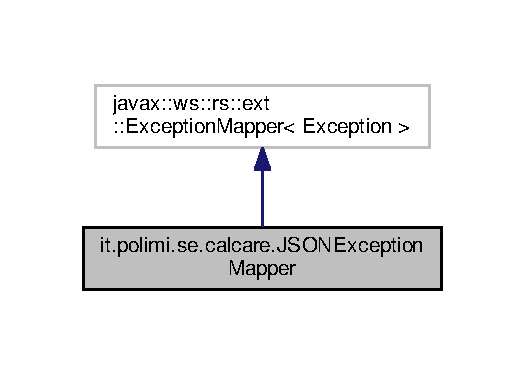
\includegraphics[width=252pt]{classit_1_1polimi_1_1se_1_1calcare_1_1JSONExceptionMapper__inherit__graph}
\end{center}
\end{figure}


Collaboration diagram for it.\+polimi.\+se.\+calcare.\+J\+S\+O\+N\+Exception\+Mapper\+:
\nopagebreak
\begin{figure}[H]
\begin{center}
\leavevmode
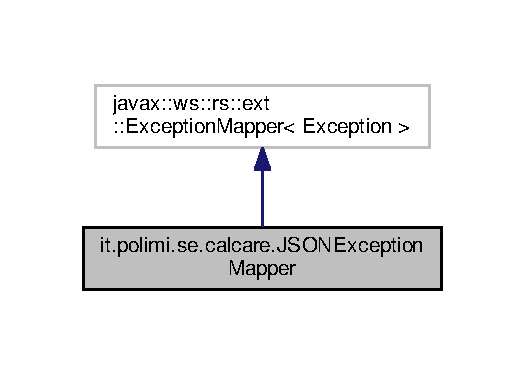
\includegraphics[width=252pt]{classit_1_1polimi_1_1se_1_1calcare_1_1JSONExceptionMapper__coll__graph}
\end{center}
\end{figure}
\subsection*{Public Member Functions}
\begin{DoxyCompactItemize}
\item 
\hypertarget{classit_1_1polimi_1_1se_1_1calcare_1_1JSONExceptionMapper_aefc6967bbea80efc0415ee0a718946d0}{}Response {\bfseries to\+Response} (Exception exception)\label{classit_1_1polimi_1_1se_1_1calcare_1_1JSONExceptionMapper_aefc6967bbea80efc0415ee0a718946d0}

\end{DoxyCompactItemize}


\subsection{Detailed Description}
\begin{DoxyAuthor}{Author}
Germano Gabbianelli 
\end{DoxyAuthor}


The documentation for this class was generated from the following file\+:\begin{DoxyCompactItemize}
\item 
src/main/java/it/polimi/se/calcare/J\+S\+O\+N\+Exception\+Mapper.\+java\end{DoxyCompactItemize}

\hypertarget{classit_1_1polimi_1_1se_1_1calcare_1_1helpers_1_1JWTHelper}{}\section{it.\+polimi.\+se.\+calcare.\+helpers.\+J\+W\+T\+Helper Class Reference}
\label{classit_1_1polimi_1_1se_1_1calcare_1_1helpers_1_1JWTHelper}\index{it.\+polimi.\+se.\+calcare.\+helpers.\+J\+W\+T\+Helper@{it.\+polimi.\+se.\+calcare.\+helpers.\+J\+W\+T\+Helper}}
\subsection*{Static Public Member Functions}
\begin{DoxyCompactItemize}
\item 
\hypertarget{classit_1_1polimi_1_1se_1_1calcare_1_1helpers_1_1JWTHelper_ab41f089e7e3ce816c53c1bfcfb05505d}{}static String {\bfseries encode} (Map$<$ String, Object $>$ map)\label{classit_1_1polimi_1_1se_1_1calcare_1_1helpers_1_1JWTHelper_ab41f089e7e3ce816c53c1bfcfb05505d}

\item 
\hypertarget{classit_1_1polimi_1_1se_1_1calcare_1_1helpers_1_1JWTHelper_a9c2d140737ed8fe485d728dd70a1a5ba}{}static String {\bfseries encode} (String key, Object value)\label{classit_1_1polimi_1_1se_1_1calcare_1_1helpers_1_1JWTHelper_a9c2d140737ed8fe485d728dd70a1a5ba}

\item 
\hypertarget{classit_1_1polimi_1_1se_1_1calcare_1_1helpers_1_1JWTHelper_a5c5b4bee0843be999a4f0287b3702348}{}static String {\bfseries encode} (String key, \hyperlink{classit_1_1polimi_1_1se_1_1calcare_1_1entities_1_1User}{User} user)\label{classit_1_1polimi_1_1se_1_1calcare_1_1helpers_1_1JWTHelper_a5c5b4bee0843be999a4f0287b3702348}

\item 
\hypertarget{classit_1_1polimi_1_1se_1_1calcare_1_1helpers_1_1JWTHelper_aa342954131b477dafc377fdc30f6f6bd}{}static Map$<$ String, Object $>$ {\bfseries decode} (String token, int status)\label{classit_1_1polimi_1_1se_1_1calcare_1_1helpers_1_1JWTHelper_aa342954131b477dafc377fdc30f6f6bd}

\item 
\hypertarget{classit_1_1polimi_1_1se_1_1calcare_1_1helpers_1_1JWTHelper_a1123aa462e87e5873a56be67f5bd4d41}{}static Map$<$ String, Object $>$ {\bfseries decode} (String token)\label{classit_1_1polimi_1_1se_1_1calcare_1_1helpers_1_1JWTHelper_a1123aa462e87e5873a56be67f5bd4d41}

\item 
\hypertarget{classit_1_1polimi_1_1se_1_1calcare_1_1helpers_1_1JWTHelper_a1e4e73764660e4849b1b91059ef00982}{}static$<$ T $>$ T {\bfseries decode} (String token, String key, int status)\label{classit_1_1polimi_1_1se_1_1calcare_1_1helpers_1_1JWTHelper_a1e4e73764660e4849b1b91059ef00982}

\item 
\hypertarget{classit_1_1polimi_1_1se_1_1calcare_1_1helpers_1_1JWTHelper_ac06dbf2975d6331717b4ae4775ffa8e1}{}static$<$ T $>$ T {\bfseries decode} (String token, String key)\label{classit_1_1polimi_1_1se_1_1calcare_1_1helpers_1_1JWTHelper_ac06dbf2975d6331717b4ae4775ffa8e1}

\end{DoxyCompactItemize}


\subsection{Detailed Description}
\begin{DoxyAuthor}{Author}
Germano Gabbianelli 
\end{DoxyAuthor}


The documentation for this class was generated from the following file\+:\begin{DoxyCompactItemize}
\item 
src/main/java/it/polimi/se/calcare/helpers/J\+W\+T\+Helper.\+java\end{DoxyCompactItemize}

\hypertarget{classit_1_1polimi_1_1se_1_1calcare_1_1entities_1_1Notification}{}\section{it.\+polimi.\+se.\+calcare.\+entities.\+Notification Class Reference}
\label{classit_1_1polimi_1_1se_1_1calcare_1_1entities_1_1Notification}\index{it.\+polimi.\+se.\+calcare.\+entities.\+Notification@{it.\+polimi.\+se.\+calcare.\+entities.\+Notification}}


Inheritance diagram for it.\+polimi.\+se.\+calcare.\+entities.\+Notification\+:
\nopagebreak
\begin{figure}[H]
\begin{center}
\leavevmode
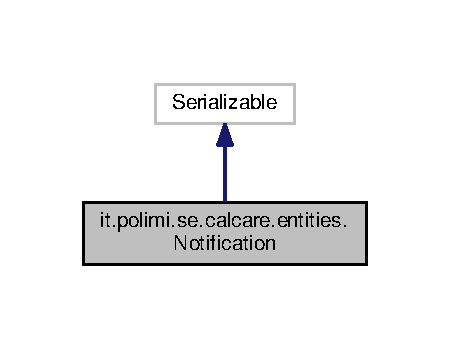
\includegraphics[width=216pt]{classit_1_1polimi_1_1se_1_1calcare_1_1entities_1_1Notification__inherit__graph}
\end{center}
\end{figure}


Collaboration diagram for it.\+polimi.\+se.\+calcare.\+entities.\+Notification\+:
\nopagebreak
\begin{figure}[H]
\begin{center}
\leavevmode
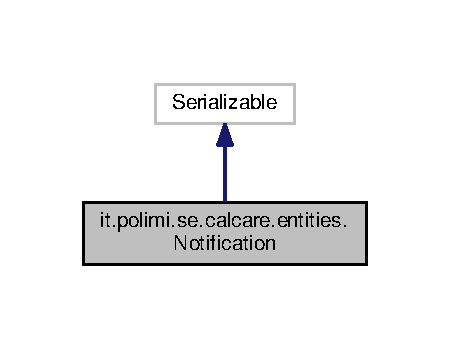
\includegraphics[width=216pt]{classit_1_1polimi_1_1se_1_1calcare_1_1entities_1_1Notification__coll__graph}
\end{center}
\end{figure}
\subsection*{Public Member Functions}
\begin{DoxyCompactItemize}
\item 
\hypertarget{classit_1_1polimi_1_1se_1_1calcare_1_1entities_1_1Notification_ad9838f50cb6a092d5501d4ddf17780d9}{}{\bfseries Notification} (\hyperlink{classit_1_1polimi_1_1se_1_1calcare_1_1entities_1_1Event}{Event} event, \hyperlink{classit_1_1polimi_1_1se_1_1calcare_1_1entities_1_1NotificationType}{Notification\+Type} type, \hyperlink{classit_1_1polimi_1_1se_1_1calcare_1_1entities_1_1User}{User} user)\label{classit_1_1polimi_1_1se_1_1calcare_1_1entities_1_1Notification_ad9838f50cb6a092d5501d4ddf17780d9}

\item 
\hypertarget{classit_1_1polimi_1_1se_1_1calcare_1_1entities_1_1Notification_acb2e2e3bed8cd7731343d4e35bdcb745}{}{\bfseries Notification} (Integer id)\label{classit_1_1polimi_1_1se_1_1calcare_1_1entities_1_1Notification_acb2e2e3bed8cd7731343d4e35bdcb745}

\item 
\hypertarget{classit_1_1polimi_1_1se_1_1calcare_1_1entities_1_1Notification_a4c9aedc5279e0a03014e33820f4d5331}{}Integer {\bfseries get\+Id} ()\label{classit_1_1polimi_1_1se_1_1calcare_1_1entities_1_1Notification_a4c9aedc5279e0a03014e33820f4d5331}

\item 
\hypertarget{classit_1_1polimi_1_1se_1_1calcare_1_1entities_1_1Notification_a79da718c17f246d6a4566f38f54604dd}{}void {\bfseries set\+Id} (Integer id)\label{classit_1_1polimi_1_1se_1_1calcare_1_1entities_1_1Notification_a79da718c17f246d6a4566f38f54604dd}

\item 
\hypertarget{classit_1_1polimi_1_1se_1_1calcare_1_1entities_1_1Notification_a1b77435517309f9839f5519e3c0ebad4}{}\hyperlink{classit_1_1polimi_1_1se_1_1calcare_1_1entities_1_1Event}{Event} {\bfseries get\+Event} ()\label{classit_1_1polimi_1_1se_1_1calcare_1_1entities_1_1Notification_a1b77435517309f9839f5519e3c0ebad4}

\item 
\hypertarget{classit_1_1polimi_1_1se_1_1calcare_1_1entities_1_1Notification_a114ac1832474e81788af9c07bdd66bce}{}void {\bfseries set\+Event} (\hyperlink{classit_1_1polimi_1_1se_1_1calcare_1_1entities_1_1Event}{Event} event)\label{classit_1_1polimi_1_1se_1_1calcare_1_1entities_1_1Notification_a114ac1832474e81788af9c07bdd66bce}

\item 
\hypertarget{classit_1_1polimi_1_1se_1_1calcare_1_1entities_1_1Notification_a971887843945f4895fa3da3ec61e4538}{}\hyperlink{classit_1_1polimi_1_1se_1_1calcare_1_1entities_1_1NotificationType}{Notification\+Type} {\bfseries get\+Type} ()\label{classit_1_1polimi_1_1se_1_1calcare_1_1entities_1_1Notification_a971887843945f4895fa3da3ec61e4538}

\item 
\hypertarget{classit_1_1polimi_1_1se_1_1calcare_1_1entities_1_1Notification_acbc2edc1331f11ffb4376771332ea151}{}void {\bfseries set\+Type} (\hyperlink{classit_1_1polimi_1_1se_1_1calcare_1_1entities_1_1NotificationType}{Notification\+Type} type)\label{classit_1_1polimi_1_1se_1_1calcare_1_1entities_1_1Notification_acbc2edc1331f11ffb4376771332ea151}

\item 
\hypertarget{classit_1_1polimi_1_1se_1_1calcare_1_1entities_1_1Notification_a74ad302ceda58a3f59bc19cd7ab38c56}{}\hyperlink{classit_1_1polimi_1_1se_1_1calcare_1_1entities_1_1User}{User} {\bfseries get\+User} ()\label{classit_1_1polimi_1_1se_1_1calcare_1_1entities_1_1Notification_a74ad302ceda58a3f59bc19cd7ab38c56}

\item 
\hypertarget{classit_1_1polimi_1_1se_1_1calcare_1_1entities_1_1Notification_a241c329e38da36c5b78b032016457044}{}void {\bfseries set\+User} (\hyperlink{classit_1_1polimi_1_1se_1_1calcare_1_1entities_1_1User}{User} user)\label{classit_1_1polimi_1_1se_1_1calcare_1_1entities_1_1Notification_a241c329e38da36c5b78b032016457044}

\item 
\hypertarget{classit_1_1polimi_1_1se_1_1calcare_1_1entities_1_1Notification_a5f86a9aa4acb578e677ecb52903aa90d}{}String {\bfseries get\+Description} ()\label{classit_1_1polimi_1_1se_1_1calcare_1_1entities_1_1Notification_a5f86a9aa4acb578e677ecb52903aa90d}

\item 
\hypertarget{classit_1_1polimi_1_1se_1_1calcare_1_1entities_1_1Notification_ace65de780413c9659a7f8db59e2a12d2}{}int {\bfseries hash\+Code} ()\label{classit_1_1polimi_1_1se_1_1calcare_1_1entities_1_1Notification_ace65de780413c9659a7f8db59e2a12d2}

\item 
\hypertarget{classit_1_1polimi_1_1se_1_1calcare_1_1entities_1_1Notification_a9446f03a7a0a4d8c2331522cc89d520d}{}boolean {\bfseries equals} (Object object)\label{classit_1_1polimi_1_1se_1_1calcare_1_1entities_1_1Notification_a9446f03a7a0a4d8c2331522cc89d520d}

\item 
\hypertarget{classit_1_1polimi_1_1se_1_1calcare_1_1entities_1_1Notification_a4b3ad27c98baffd0707dd7075ab865d0}{}String {\bfseries to\+String} ()\label{classit_1_1polimi_1_1se_1_1calcare_1_1entities_1_1Notification_a4b3ad27c98baffd0707dd7075ab865d0}

\end{DoxyCompactItemize}


\subsection{Detailed Description}
\begin{DoxyAuthor}{Author}
tyrion 
\end{DoxyAuthor}


The documentation for this class was generated from the following file\+:\begin{DoxyCompactItemize}
\item 
src/main/java/it/polimi/se/calcare/entities/Notification.\+java\end{DoxyCompactItemize}

\hypertarget{classit_1_1polimi_1_1se_1_1calcare_1_1service_1_1NotificationFacadeREST}{}\section{it.\+polimi.\+se.\+calcare.\+service.\+Notification\+Facade\+R\+E\+S\+T Class Reference}
\label{classit_1_1polimi_1_1se_1_1calcare_1_1service_1_1NotificationFacadeREST}\index{it.\+polimi.\+se.\+calcare.\+service.\+Notification\+Facade\+R\+E\+S\+T@{it.\+polimi.\+se.\+calcare.\+service.\+Notification\+Facade\+R\+E\+S\+T}}


Inheritance diagram for it.\+polimi.\+se.\+calcare.\+service.\+Notification\+Facade\+R\+E\+S\+T\+:
\nopagebreak
\begin{figure}[H]
\begin{center}
\leavevmode
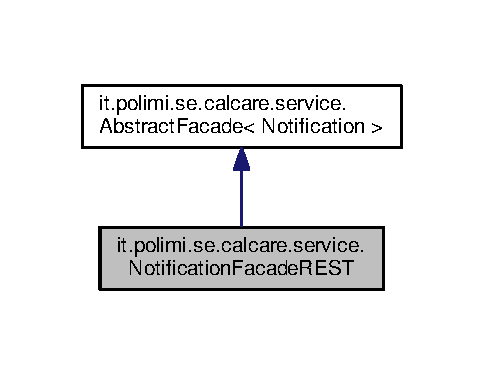
\includegraphics[width=232pt]{classit_1_1polimi_1_1se_1_1calcare_1_1service_1_1NotificationFacadeREST__inherit__graph}
\end{center}
\end{figure}


Collaboration diagram for it.\+polimi.\+se.\+calcare.\+service.\+Notification\+Facade\+R\+E\+S\+T\+:
\nopagebreak
\begin{figure}[H]
\begin{center}
\leavevmode
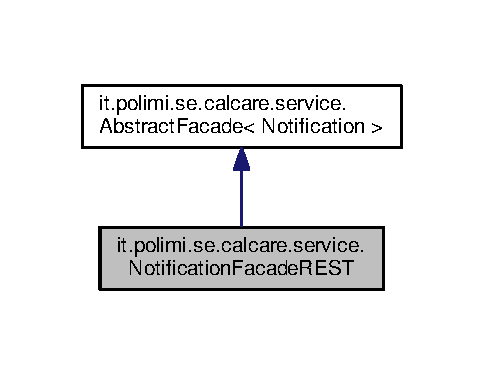
\includegraphics[width=232pt]{classit_1_1polimi_1_1se_1_1calcare_1_1service_1_1NotificationFacadeREST__coll__graph}
\end{center}
\end{figure}
\subsection*{Public Member Functions}
\begin{DoxyCompactItemize}
\item 
\hypertarget{classit_1_1polimi_1_1se_1_1calcare_1_1service_1_1NotificationFacadeREST_afc9a695d34cfc09011a34893409cf355}{}List$<$ \hyperlink{classit_1_1polimi_1_1se_1_1calcare_1_1entities_1_1Notification}{Notification} $>$ {\bfseries find\+All} (@Context Security\+Context sc)\label{classit_1_1polimi_1_1se_1_1calcare_1_1service_1_1NotificationFacadeREST_afc9a695d34cfc09011a34893409cf355}

\end{DoxyCompactItemize}
\subsection*{Protected Member Functions}
\begin{DoxyCompactItemize}
\item 
\hypertarget{classit_1_1polimi_1_1se_1_1calcare_1_1service_1_1NotificationFacadeREST_a57a4f68684a2d4df6d212e4bc95e2060}{}Entity\+Manager {\bfseries get\+Entity\+Manager} ()\label{classit_1_1polimi_1_1se_1_1calcare_1_1service_1_1NotificationFacadeREST_a57a4f68684a2d4df6d212e4bc95e2060}

\end{DoxyCompactItemize}


\subsection{Detailed Description}
\begin{DoxyAuthor}{Author}
tyrion 
\end{DoxyAuthor}


The documentation for this class was generated from the following file\+:\begin{DoxyCompactItemize}
\item 
src/main/java/it/polimi/se/calcare/service/Notification\+Facade\+R\+E\+S\+T.\+java\end{DoxyCompactItemize}

\hypertarget{classit_1_1polimi_1_1se_1_1calcare_1_1helpers_1_1NotificationHelper}{}\section{it.\+polimi.\+se.\+calcare.\+helpers.\+Notification\+Helper Class Reference}
\label{classit_1_1polimi_1_1se_1_1calcare_1_1helpers_1_1NotificationHelper}\index{it.\+polimi.\+se.\+calcare.\+helpers.\+Notification\+Helper@{it.\+polimi.\+se.\+calcare.\+helpers.\+Notification\+Helper}}
\subsection*{Public Member Functions}
\begin{DoxyCompactItemize}
\item 
\hypertarget{classit_1_1polimi_1_1se_1_1calcare_1_1helpers_1_1NotificationHelper_a6f2aa75f90988ad98887361fe336af60}{}{\bfseries Notification\+Helper} (Entity\+Manager em, Notification\+Type.\+Enum type, \hyperlink{classit_1_1polimi_1_1se_1_1calcare_1_1entities_1_1Event}{Event} event)\label{classit_1_1polimi_1_1se_1_1calcare_1_1helpers_1_1NotificationHelper_a6f2aa75f90988ad98887361fe336af60}

\item 
\hypertarget{classit_1_1polimi_1_1se_1_1calcare_1_1helpers_1_1NotificationHelper_a4577f62220db3084bf93e6ccf646c69a}{}\hyperlink{classit_1_1polimi_1_1se_1_1calcare_1_1entities_1_1Notification}{Notification} {\bfseries send\+To} (\hyperlink{classit_1_1polimi_1_1se_1_1calcare_1_1entities_1_1User}{User} user, U\+R\+I link, Object...\+args)\label{classit_1_1polimi_1_1se_1_1calcare_1_1helpers_1_1NotificationHelper_a4577f62220db3084bf93e6ccf646c69a}

\item 
\hypertarget{classit_1_1polimi_1_1se_1_1calcare_1_1helpers_1_1NotificationHelper_adaddb6170e1c623d0358f52e75cef76d}{}\hyperlink{classit_1_1polimi_1_1se_1_1calcare_1_1entities_1_1Notification}{Notification} {\bfseries send\+To} (\hyperlink{classit_1_1polimi_1_1se_1_1calcare_1_1entities_1_1User}{User} user, String link, Object...\+args)\label{classit_1_1polimi_1_1se_1_1calcare_1_1helpers_1_1NotificationHelper_adaddb6170e1c623d0358f52e75cef76d}

\end{DoxyCompactItemize}


\subsection{Detailed Description}
\begin{DoxyAuthor}{Author}
Germano Gabbianelli 
\end{DoxyAuthor}


The documentation for this class was generated from the following file\+:\begin{DoxyCompactItemize}
\item 
src/main/java/it/polimi/se/calcare/helpers/Notification\+Helper.\+java\end{DoxyCompactItemize}

\hypertarget{classit_1_1polimi_1_1se_1_1calcare_1_1entities_1_1NotificationType}{}\section{it.\+polimi.\+se.\+calcare.\+entities.\+Notification\+Type Class Reference}
\label{classit_1_1polimi_1_1se_1_1calcare_1_1entities_1_1NotificationType}\index{it.\+polimi.\+se.\+calcare.\+entities.\+Notification\+Type@{it.\+polimi.\+se.\+calcare.\+entities.\+Notification\+Type}}


Inheritance diagram for it.\+polimi.\+se.\+calcare.\+entities.\+Notification\+Type\+:
\nopagebreak
\begin{figure}[H]
\begin{center}
\leavevmode
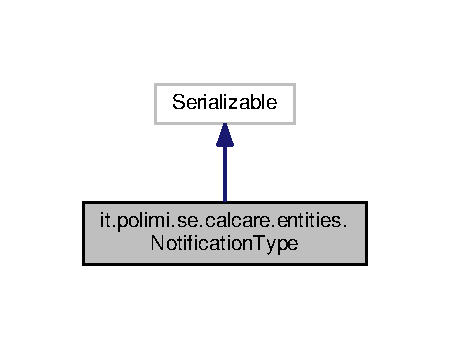
\includegraphics[width=216pt]{classit_1_1polimi_1_1se_1_1calcare_1_1entities_1_1NotificationType__inherit__graph}
\end{center}
\end{figure}


Collaboration diagram for it.\+polimi.\+se.\+calcare.\+entities.\+Notification\+Type\+:
\nopagebreak
\begin{figure}[H]
\begin{center}
\leavevmode
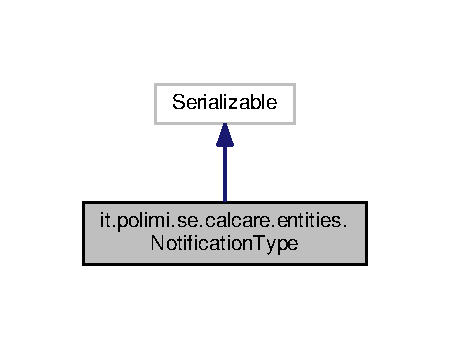
\includegraphics[width=216pt]{classit_1_1polimi_1_1se_1_1calcare_1_1entities_1_1NotificationType__coll__graph}
\end{center}
\end{figure}
\subsection*{Classes}
\begin{DoxyCompactItemize}
\item 
enum \hyperlink{enumit_1_1polimi_1_1se_1_1calcare_1_1entities_1_1NotificationType_1_1Enum}{Enum}
\end{DoxyCompactItemize}
\subsection*{Public Member Functions}
\begin{DoxyCompactItemize}
\item 
\hypertarget{classit_1_1polimi_1_1se_1_1calcare_1_1entities_1_1NotificationType_ab6c7b3c6cabb34e7769f175e7cb80573}{}{\bfseries Notification\+Type} (Integer id)\label{classit_1_1polimi_1_1se_1_1calcare_1_1entities_1_1NotificationType_ab6c7b3c6cabb34e7769f175e7cb80573}

\item 
\hypertarget{classit_1_1polimi_1_1se_1_1calcare_1_1entities_1_1NotificationType_a1fa03f7fb0fbfc21f7ac3749406c79f8}{}{\bfseries Notification\+Type} (Integer id, String name, String description)\label{classit_1_1polimi_1_1se_1_1calcare_1_1entities_1_1NotificationType_a1fa03f7fb0fbfc21f7ac3749406c79f8}

\item 
\hypertarget{classit_1_1polimi_1_1se_1_1calcare_1_1entities_1_1NotificationType_a8271d2e440430978423dc228adb76e55}{}Integer {\bfseries get\+Id} ()\label{classit_1_1polimi_1_1se_1_1calcare_1_1entities_1_1NotificationType_a8271d2e440430978423dc228adb76e55}

\item 
\hypertarget{classit_1_1polimi_1_1se_1_1calcare_1_1entities_1_1NotificationType_ac9087bee566bf31c9f06c81f8e9ae6c7}{}void {\bfseries set\+Id} (Integer id)\label{classit_1_1polimi_1_1se_1_1calcare_1_1entities_1_1NotificationType_ac9087bee566bf31c9f06c81f8e9ae6c7}

\item 
\hypertarget{classit_1_1polimi_1_1se_1_1calcare_1_1entities_1_1NotificationType_a000d0e0ad670bc07dab38a2f98397bd8}{}String {\bfseries get\+Name} ()\label{classit_1_1polimi_1_1se_1_1calcare_1_1entities_1_1NotificationType_a000d0e0ad670bc07dab38a2f98397bd8}

\item 
\hypertarget{classit_1_1polimi_1_1se_1_1calcare_1_1entities_1_1NotificationType_a2170dc67222379ca75fd7dcef59e0457}{}void {\bfseries set\+Name} (String name)\label{classit_1_1polimi_1_1se_1_1calcare_1_1entities_1_1NotificationType_a2170dc67222379ca75fd7dcef59e0457}

\item 
\hypertarget{classit_1_1polimi_1_1se_1_1calcare_1_1entities_1_1NotificationType_a3f729343d563bab3dbaf5cef06d31f82}{}String {\bfseries get\+Description} ()\label{classit_1_1polimi_1_1se_1_1calcare_1_1entities_1_1NotificationType_a3f729343d563bab3dbaf5cef06d31f82}

\item 
\hypertarget{classit_1_1polimi_1_1se_1_1calcare_1_1entities_1_1NotificationType_a96b9cf4f31dc54298543445031a9f974}{}void {\bfseries set\+Description} (String description)\label{classit_1_1polimi_1_1se_1_1calcare_1_1entities_1_1NotificationType_a96b9cf4f31dc54298543445031a9f974}

\item 
\hypertarget{classit_1_1polimi_1_1se_1_1calcare_1_1entities_1_1NotificationType_a34f6fa9d4f8f728a0bf69f806463a4b4}{}Collection$<$ \hyperlink{classit_1_1polimi_1_1se_1_1calcare_1_1entities_1_1Notification}{Notification} $>$ {\bfseries get\+Notification\+Collection} ()\label{classit_1_1polimi_1_1se_1_1calcare_1_1entities_1_1NotificationType_a34f6fa9d4f8f728a0bf69f806463a4b4}

\item 
\hypertarget{classit_1_1polimi_1_1se_1_1calcare_1_1entities_1_1NotificationType_a2642f5dda02b3bcc0e409fe1a838cd7b}{}void {\bfseries set\+Notification\+Collection} (Collection$<$ \hyperlink{classit_1_1polimi_1_1se_1_1calcare_1_1entities_1_1Notification}{Notification} $>$ notification\+Collection)\label{classit_1_1polimi_1_1se_1_1calcare_1_1entities_1_1NotificationType_a2642f5dda02b3bcc0e409fe1a838cd7b}

\item 
\hypertarget{classit_1_1polimi_1_1se_1_1calcare_1_1entities_1_1NotificationType_a3206f3cbc6bd16950d89f031a9f64ea7}{}int {\bfseries hash\+Code} ()\label{classit_1_1polimi_1_1se_1_1calcare_1_1entities_1_1NotificationType_a3206f3cbc6bd16950d89f031a9f64ea7}

\item 
\hypertarget{classit_1_1polimi_1_1se_1_1calcare_1_1entities_1_1NotificationType_a9eadd688e32a63c7d2aae143d66ade92}{}boolean {\bfseries equals} (Object object)\label{classit_1_1polimi_1_1se_1_1calcare_1_1entities_1_1NotificationType_a9eadd688e32a63c7d2aae143d66ade92}

\item 
\hypertarget{classit_1_1polimi_1_1se_1_1calcare_1_1entities_1_1NotificationType_a4fe08a6ab31b6c22e165cc162f77ec70}{}String {\bfseries to\+String} ()\label{classit_1_1polimi_1_1se_1_1calcare_1_1entities_1_1NotificationType_a4fe08a6ab31b6c22e165cc162f77ec70}

\end{DoxyCompactItemize}


\subsection{Detailed Description}
\begin{DoxyAuthor}{Author}
tyrion 
\end{DoxyAuthor}


The documentation for this class was generated from the following file\+:\begin{DoxyCompactItemize}
\item 
src/main/java/it/polimi/se/calcare/entities/Notification\+Type.\+java\end{DoxyCompactItemize}

\hypertarget{classit_1_1polimi_1_1se_1_1calcare_1_1entities_1_1Participation}{}\section{it.\+polimi.\+se.\+calcare.\+entities.\+Participation Class Reference}
\label{classit_1_1polimi_1_1se_1_1calcare_1_1entities_1_1Participation}\index{it.\+polimi.\+se.\+calcare.\+entities.\+Participation@{it.\+polimi.\+se.\+calcare.\+entities.\+Participation}}


Inheritance diagram for it.\+polimi.\+se.\+calcare.\+entities.\+Participation\+:
\nopagebreak
\begin{figure}[H]
\begin{center}
\leavevmode
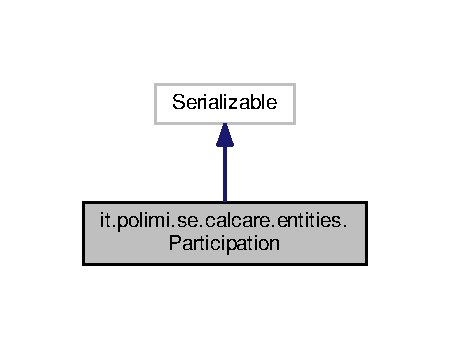
\includegraphics[width=216pt]{classit_1_1polimi_1_1se_1_1calcare_1_1entities_1_1Participation__inherit__graph}
\end{center}
\end{figure}


Collaboration diagram for it.\+polimi.\+se.\+calcare.\+entities.\+Participation\+:
\nopagebreak
\begin{figure}[H]
\begin{center}
\leavevmode
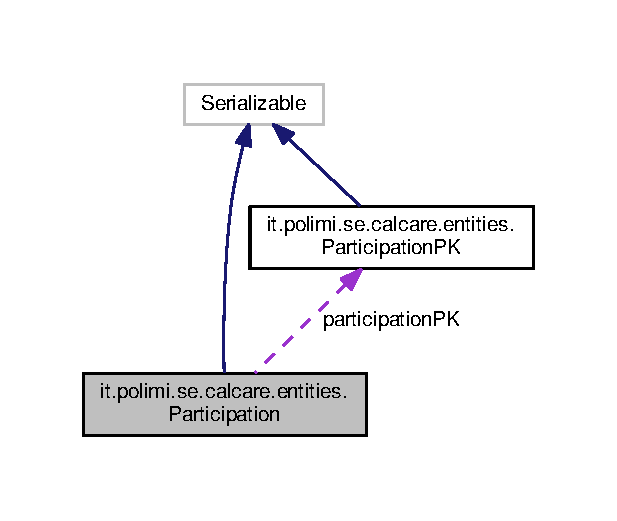
\includegraphics[width=296pt]{classit_1_1polimi_1_1se_1_1calcare_1_1entities_1_1Participation__coll__graph}
\end{center}
\end{figure}
\subsection*{Public Member Functions}
\begin{DoxyCompactItemize}
\item 
\hypertarget{classit_1_1polimi_1_1se_1_1calcare_1_1entities_1_1Participation_a7e532a6d192f9303b7f6fd4e7761fe37}{}{\bfseries Participation} (\hyperlink{classit_1_1polimi_1_1se_1_1calcare_1_1entities_1_1ParticipationPK}{Participation\+P\+K} participation\+P\+K)\label{classit_1_1polimi_1_1se_1_1calcare_1_1entities_1_1Participation_a7e532a6d192f9303b7f6fd4e7761fe37}

\item 
\hypertarget{classit_1_1polimi_1_1se_1_1calcare_1_1entities_1_1Participation_aafba461963c58c87c05405e1c4e27e34}{}{\bfseries Participation} (int event, int calendars\+Id)\label{classit_1_1polimi_1_1se_1_1calcare_1_1entities_1_1Participation_aafba461963c58c87c05405e1c4e27e34}

\item 
\hypertarget{classit_1_1polimi_1_1se_1_1calcare_1_1entities_1_1Participation_aadae0e28354b3315d7482ec67337a788}{}{\bfseries Participation} (int event, int calendars\+Id, Boolean accepted)\label{classit_1_1polimi_1_1se_1_1calcare_1_1entities_1_1Participation_aadae0e28354b3315d7482ec67337a788}

\item 
\hypertarget{classit_1_1polimi_1_1se_1_1calcare_1_1entities_1_1Participation_aeffa99d60edf659e95e524de1b7840a9}{}{\bfseries Participation} (\hyperlink{classit_1_1polimi_1_1se_1_1calcare_1_1entities_1_1Event}{Event} event, \hyperlink{classit_1_1polimi_1_1se_1_1calcare_1_1entities_1_1Calendar}{Calendar} calendar, Boolean accepted)\label{classit_1_1polimi_1_1se_1_1calcare_1_1entities_1_1Participation_aeffa99d60edf659e95e524de1b7840a9}

\item 
\hypertarget{classit_1_1polimi_1_1se_1_1calcare_1_1entities_1_1Participation_a532c4c1409b1e89eed0ddcfd94ffabc6}{}{\bfseries Participation} (\hyperlink{classit_1_1polimi_1_1se_1_1calcare_1_1entities_1_1Event}{Event} event, \hyperlink{classit_1_1polimi_1_1se_1_1calcare_1_1entities_1_1Calendar}{Calendar} calendar)\label{classit_1_1polimi_1_1se_1_1calcare_1_1entities_1_1Participation_a532c4c1409b1e89eed0ddcfd94ffabc6}

\item 
\hypertarget{classit_1_1polimi_1_1se_1_1calcare_1_1entities_1_1Participation_a613b77b59198acc02772ef951b0d66d3}{}\hyperlink{classit_1_1polimi_1_1se_1_1calcare_1_1entities_1_1ParticipationPK}{Participation\+P\+K} {\bfseries get\+Participation\+P\+K} ()\label{classit_1_1polimi_1_1se_1_1calcare_1_1entities_1_1Participation_a613b77b59198acc02772ef951b0d66d3}

\item 
\hypertarget{classit_1_1polimi_1_1se_1_1calcare_1_1entities_1_1Participation_a76a2994dd3501a06c41f3049fde61506}{}void {\bfseries set\+Participation\+P\+K} (\hyperlink{classit_1_1polimi_1_1se_1_1calcare_1_1entities_1_1ParticipationPK}{Participation\+P\+K} participation\+P\+K)\label{classit_1_1polimi_1_1se_1_1calcare_1_1entities_1_1Participation_a76a2994dd3501a06c41f3049fde61506}

\item 
\hypertarget{classit_1_1polimi_1_1se_1_1calcare_1_1entities_1_1Participation_acac1a53247d421e91b895d5b2af3771b}{}Boolean {\bfseries get\+Accepted} ()\label{classit_1_1polimi_1_1se_1_1calcare_1_1entities_1_1Participation_acac1a53247d421e91b895d5b2af3771b}

\item 
\hypertarget{classit_1_1polimi_1_1se_1_1calcare_1_1entities_1_1Participation_a0d73e9a0dcddc52223279d469f46e7f2}{}void {\bfseries set\+Accepted} (Boolean accepted)\label{classit_1_1polimi_1_1se_1_1calcare_1_1entities_1_1Participation_a0d73e9a0dcddc52223279d469f46e7f2}

\item 
\hypertarget{classit_1_1polimi_1_1se_1_1calcare_1_1entities_1_1Participation_a0f44c43fef48a7d21166a8a41324928e}{}\hyperlink{classit_1_1polimi_1_1se_1_1calcare_1_1entities_1_1Calendar}{Calendar} {\bfseries get\+Calendar} ()\label{classit_1_1polimi_1_1se_1_1calcare_1_1entities_1_1Participation_a0f44c43fef48a7d21166a8a41324928e}

\item 
\hypertarget{classit_1_1polimi_1_1se_1_1calcare_1_1entities_1_1Participation_abc3ecf19db5698986db4dbc7f90eacce}{}void {\bfseries set\+Calendar} (\hyperlink{classit_1_1polimi_1_1se_1_1calcare_1_1entities_1_1Calendar}{Calendar} calendar)\label{classit_1_1polimi_1_1se_1_1calcare_1_1entities_1_1Participation_abc3ecf19db5698986db4dbc7f90eacce}

\item 
\hypertarget{classit_1_1polimi_1_1se_1_1calcare_1_1entities_1_1Participation_a6663d5f2d55d1c96f3d46be1e5f615f4}{}\hyperlink{classit_1_1polimi_1_1se_1_1calcare_1_1entities_1_1Event}{Event} {\bfseries get\+Event} ()\label{classit_1_1polimi_1_1se_1_1calcare_1_1entities_1_1Participation_a6663d5f2d55d1c96f3d46be1e5f615f4}

\item 
\hypertarget{classit_1_1polimi_1_1se_1_1calcare_1_1entities_1_1Participation_a032d1eff7ec2944a9f95c382efb94c92}{}void {\bfseries set\+Event} (\hyperlink{classit_1_1polimi_1_1se_1_1calcare_1_1entities_1_1Event}{Event} event)\label{classit_1_1polimi_1_1se_1_1calcare_1_1entities_1_1Participation_a032d1eff7ec2944a9f95c382efb94c92}

\item 
\hypertarget{classit_1_1polimi_1_1se_1_1calcare_1_1entities_1_1Participation_a70475620dcf88a8623c7d6ecf01c6ed8}{}\hyperlink{classit_1_1polimi_1_1se_1_1calcare_1_1entities_1_1User}{User} {\bfseries get\+User} ()\label{classit_1_1polimi_1_1se_1_1calcare_1_1entities_1_1Participation_a70475620dcf88a8623c7d6ecf01c6ed8}

\item 
\hypertarget{classit_1_1polimi_1_1se_1_1calcare_1_1entities_1_1Participation_a334e522c225615fbdaa62ace08dbbe2d}{}int {\bfseries hash\+Code} ()\label{classit_1_1polimi_1_1se_1_1calcare_1_1entities_1_1Participation_a334e522c225615fbdaa62ace08dbbe2d}

\item 
\hypertarget{classit_1_1polimi_1_1se_1_1calcare_1_1entities_1_1Participation_ae639c999f0406771378a8a38ebaf512c}{}boolean {\bfseries equals} (Object object)\label{classit_1_1polimi_1_1se_1_1calcare_1_1entities_1_1Participation_ae639c999f0406771378a8a38ebaf512c}

\item 
\hypertarget{classit_1_1polimi_1_1se_1_1calcare_1_1entities_1_1Participation_a065698dc991ca94224b7c2d1ba54f874}{}String {\bfseries to\+String} ()\label{classit_1_1polimi_1_1se_1_1calcare_1_1entities_1_1Participation_a065698dc991ca94224b7c2d1ba54f874}

\end{DoxyCompactItemize}
\subsection*{Protected Attributes}
\begin{DoxyCompactItemize}
\item 
\hypertarget{classit_1_1polimi_1_1se_1_1calcare_1_1entities_1_1Participation_a050a2c5040fc31b205ddf57a940bc8b4}{}\hyperlink{classit_1_1polimi_1_1se_1_1calcare_1_1entities_1_1ParticipationPK}{Participation\+P\+K} {\bfseries participation\+P\+K}\label{classit_1_1polimi_1_1se_1_1calcare_1_1entities_1_1Participation_a050a2c5040fc31b205ddf57a940bc8b4}

\end{DoxyCompactItemize}


\subsection{Detailed Description}
\begin{DoxyAuthor}{Author}
tyrion 
\end{DoxyAuthor}


The documentation for this class was generated from the following file\+:\begin{DoxyCompactItemize}
\item 
src/main/java/it/polimi/se/calcare/entities/Participation.\+java\end{DoxyCompactItemize}

\hypertarget{classit_1_1polimi_1_1se_1_1calcare_1_1service_1_1ParticipationFacadeREST}{}\section{it.\+polimi.\+se.\+calcare.\+service.\+Participation\+Facade\+R\+E\+S\+T Class Reference}
\label{classit_1_1polimi_1_1se_1_1calcare_1_1service_1_1ParticipationFacadeREST}\index{it.\+polimi.\+se.\+calcare.\+service.\+Participation\+Facade\+R\+E\+S\+T@{it.\+polimi.\+se.\+calcare.\+service.\+Participation\+Facade\+R\+E\+S\+T}}


Inheritance diagram for it.\+polimi.\+se.\+calcare.\+service.\+Participation\+Facade\+R\+E\+S\+T\+:
\nopagebreak
\begin{figure}[H]
\begin{center}
\leavevmode
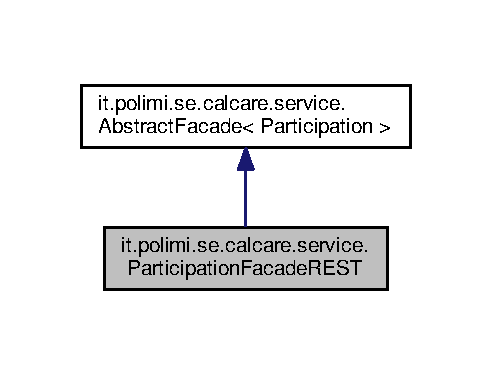
\includegraphics[width=236pt]{classit_1_1polimi_1_1se_1_1calcare_1_1service_1_1ParticipationFacadeREST__inherit__graph}
\end{center}
\end{figure}


Collaboration diagram for it.\+polimi.\+se.\+calcare.\+service.\+Participation\+Facade\+R\+E\+S\+T\+:
\nopagebreak
\begin{figure}[H]
\begin{center}
\leavevmode
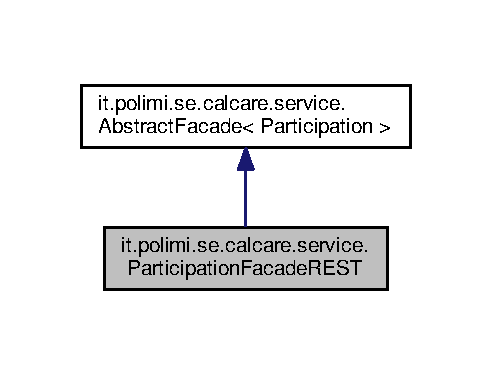
\includegraphics[width=236pt]{classit_1_1polimi_1_1se_1_1calcare_1_1service_1_1ParticipationFacadeREST__coll__graph}
\end{center}
\end{figure}
\subsection*{Public Member Functions}
\begin{DoxyCompactItemize}
\item 
\hypertarget{classit_1_1polimi_1_1se_1_1calcare_1_1service_1_1ParticipationFacadeREST_ad66ef6ae00fa44f7275a504fa6f1d34e}{}void {\bfseries create} (\hyperlink{classit_1_1polimi_1_1se_1_1calcare_1_1entities_1_1Participation}{Participation} entity)\label{classit_1_1polimi_1_1se_1_1calcare_1_1service_1_1ParticipationFacadeREST_ad66ef6ae00fa44f7275a504fa6f1d34e}

\item 
\hypertarget{classit_1_1polimi_1_1se_1_1calcare_1_1service_1_1ParticipationFacadeREST_ac61a16352690a334465adfbed8c7f78e}{}void {\bfseries edit} (@Path\+Param(\char`\"{}id\char`\"{}) Path\+Segment id, \hyperlink{classit_1_1polimi_1_1se_1_1calcare_1_1entities_1_1Participation}{Participation} entity)\label{classit_1_1polimi_1_1se_1_1calcare_1_1service_1_1ParticipationFacadeREST_ac61a16352690a334465adfbed8c7f78e}

\item 
\hypertarget{classit_1_1polimi_1_1se_1_1calcare_1_1service_1_1ParticipationFacadeREST_a1247a610f3fc58202200d09a21b1a966}{}void {\bfseries remove} (@Path\+Param(\char`\"{}id\char`\"{}) Path\+Segment id)\label{classit_1_1polimi_1_1se_1_1calcare_1_1service_1_1ParticipationFacadeREST_a1247a610f3fc58202200d09a21b1a966}

\item 
\hypertarget{classit_1_1polimi_1_1se_1_1calcare_1_1service_1_1ParticipationFacadeREST_a78d63641dc07c3c836bbc7a53859ab0a}{}\hyperlink{classit_1_1polimi_1_1se_1_1calcare_1_1entities_1_1Participation}{Participation} {\bfseries find} (@Path\+Param(\char`\"{}id\char`\"{}) Path\+Segment id)\label{classit_1_1polimi_1_1se_1_1calcare_1_1service_1_1ParticipationFacadeREST_a78d63641dc07c3c836bbc7a53859ab0a}

\item 
\hypertarget{classit_1_1polimi_1_1se_1_1calcare_1_1service_1_1ParticipationFacadeREST_af2359548d978a75d2bfe897252d8f07e}{}List$<$ \hyperlink{classit_1_1polimi_1_1se_1_1calcare_1_1entities_1_1Participation}{Participation} $>$ {\bfseries find\+All} ()\label{classit_1_1polimi_1_1se_1_1calcare_1_1service_1_1ParticipationFacadeREST_af2359548d978a75d2bfe897252d8f07e}

\item 
\hypertarget{classit_1_1polimi_1_1se_1_1calcare_1_1service_1_1ParticipationFacadeREST_a30b8c1b62f74dbc7c774c59f0425959e}{}List$<$ \hyperlink{classit_1_1polimi_1_1se_1_1calcare_1_1entities_1_1Participation}{Participation} $>$ {\bfseries find\+Range} (@Path\+Param(\char`\"{}from\char`\"{}) Integer from,@Path\+Param(\char`\"{}to\char`\"{}) Integer to)\label{classit_1_1polimi_1_1se_1_1calcare_1_1service_1_1ParticipationFacadeREST_a30b8c1b62f74dbc7c774c59f0425959e}

\item 
\hypertarget{classit_1_1polimi_1_1se_1_1calcare_1_1service_1_1ParticipationFacadeREST_aec65de4398b2e968d8ba3b4ad40435bf}{}String {\bfseries count\+R\+E\+S\+T} ()\label{classit_1_1polimi_1_1se_1_1calcare_1_1service_1_1ParticipationFacadeREST_aec65de4398b2e968d8ba3b4ad40435bf}

\end{DoxyCompactItemize}
\subsection*{Protected Member Functions}
\begin{DoxyCompactItemize}
\item 
\hypertarget{classit_1_1polimi_1_1se_1_1calcare_1_1service_1_1ParticipationFacadeREST_a0b0b8947c01c77d3650f26524c450d18}{}Entity\+Manager {\bfseries get\+Entity\+Manager} ()\label{classit_1_1polimi_1_1se_1_1calcare_1_1service_1_1ParticipationFacadeREST_a0b0b8947c01c77d3650f26524c450d18}

\end{DoxyCompactItemize}


\subsection{Detailed Description}
\begin{DoxyAuthor}{Author}
tyrion 
\end{DoxyAuthor}


The documentation for this class was generated from the following file\+:\begin{DoxyCompactItemize}
\item 
src/main/java/it/polimi/se/calcare/service/Participation\+Facade\+R\+E\+S\+T.\+java\end{DoxyCompactItemize}

\hypertarget{classit_1_1polimi_1_1se_1_1calcare_1_1entities_1_1ParticipationPK}{}\section{it.\+polimi.\+se.\+calcare.\+entities.\+Participation\+P\+K Class Reference}
\label{classit_1_1polimi_1_1se_1_1calcare_1_1entities_1_1ParticipationPK}\index{it.\+polimi.\+se.\+calcare.\+entities.\+Participation\+P\+K@{it.\+polimi.\+se.\+calcare.\+entities.\+Participation\+P\+K}}


Inheritance diagram for it.\+polimi.\+se.\+calcare.\+entities.\+Participation\+P\+K\+:
\nopagebreak
\begin{figure}[H]
\begin{center}
\leavevmode
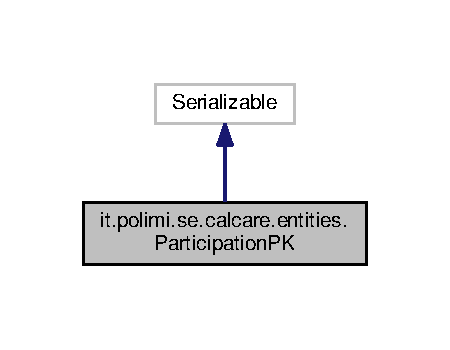
\includegraphics[width=216pt]{classit_1_1polimi_1_1se_1_1calcare_1_1entities_1_1ParticipationPK__inherit__graph}
\end{center}
\end{figure}


Collaboration diagram for it.\+polimi.\+se.\+calcare.\+entities.\+Participation\+P\+K\+:
\nopagebreak
\begin{figure}[H]
\begin{center}
\leavevmode
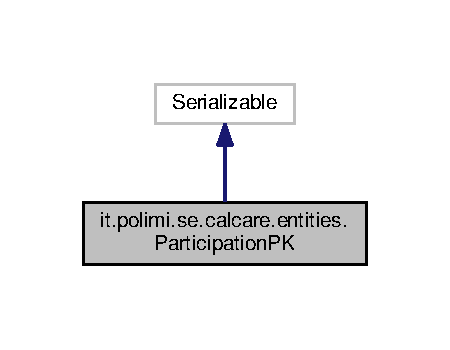
\includegraphics[width=216pt]{classit_1_1polimi_1_1se_1_1calcare_1_1entities_1_1ParticipationPK__coll__graph}
\end{center}
\end{figure}
\subsection*{Public Member Functions}
\begin{DoxyCompactItemize}
\item 
\hypertarget{classit_1_1polimi_1_1se_1_1calcare_1_1entities_1_1ParticipationPK_aa8825ec4c15056f595fbfb616f1c2d73}{}{\bfseries Participation\+P\+K} (int event, int calendars\+Id)\label{classit_1_1polimi_1_1se_1_1calcare_1_1entities_1_1ParticipationPK_aa8825ec4c15056f595fbfb616f1c2d73}

\item 
\hypertarget{classit_1_1polimi_1_1se_1_1calcare_1_1entities_1_1ParticipationPK_abd5ba3c63caed8abcc4409321d2ca461}{}int {\bfseries get\+Event} ()\label{classit_1_1polimi_1_1se_1_1calcare_1_1entities_1_1ParticipationPK_abd5ba3c63caed8abcc4409321d2ca461}

\item 
\hypertarget{classit_1_1polimi_1_1se_1_1calcare_1_1entities_1_1ParticipationPK_a09d8a6c73ab74a5ff1469f62c9b1096f}{}void {\bfseries set\+Event} (int event)\label{classit_1_1polimi_1_1se_1_1calcare_1_1entities_1_1ParticipationPK_a09d8a6c73ab74a5ff1469f62c9b1096f}

\item 
\hypertarget{classit_1_1polimi_1_1se_1_1calcare_1_1entities_1_1ParticipationPK_a82163b5aa831027ccab27a83a9257f89}{}int {\bfseries get\+Calendars\+Id} ()\label{classit_1_1polimi_1_1se_1_1calcare_1_1entities_1_1ParticipationPK_a82163b5aa831027ccab27a83a9257f89}

\item 
\hypertarget{classit_1_1polimi_1_1se_1_1calcare_1_1entities_1_1ParticipationPK_a1dfe423fdc08d1dde50f240ea28f82bc}{}void {\bfseries set\+Calendars\+Id} (int calendars\+Id)\label{classit_1_1polimi_1_1se_1_1calcare_1_1entities_1_1ParticipationPK_a1dfe423fdc08d1dde50f240ea28f82bc}

\item 
\hypertarget{classit_1_1polimi_1_1se_1_1calcare_1_1entities_1_1ParticipationPK_ad848a06e78e5a149d1197e36b30f649e}{}int {\bfseries hash\+Code} ()\label{classit_1_1polimi_1_1se_1_1calcare_1_1entities_1_1ParticipationPK_ad848a06e78e5a149d1197e36b30f649e}

\item 
\hypertarget{classit_1_1polimi_1_1se_1_1calcare_1_1entities_1_1ParticipationPK_a4e987a1134e19ebf54438d7493bf32f0}{}boolean {\bfseries equals} (Object object)\label{classit_1_1polimi_1_1se_1_1calcare_1_1entities_1_1ParticipationPK_a4e987a1134e19ebf54438d7493bf32f0}

\item 
\hypertarget{classit_1_1polimi_1_1se_1_1calcare_1_1entities_1_1ParticipationPK_ad086feb835610f54ffc557a767d60081}{}String {\bfseries to\+String} ()\label{classit_1_1polimi_1_1se_1_1calcare_1_1entities_1_1ParticipationPK_ad086feb835610f54ffc557a767d60081}

\end{DoxyCompactItemize}


\subsection{Detailed Description}
\begin{DoxyAuthor}{Author}
tyrion 
\end{DoxyAuthor}


The documentation for this class was generated from the following file\+:\begin{DoxyCompactItemize}
\item 
src/main/java/it/polimi/se/calcare/entities/Participation\+P\+K.\+java\end{DoxyCompactItemize}

\hypertarget{classit_1_1polimi_1_1se_1_1calcare_1_1auth_1_1Password}{}\section{it.\+polimi.\+se.\+calcare.\+auth.\+Password Class Reference}
\label{classit_1_1polimi_1_1se_1_1calcare_1_1auth_1_1Password}\index{it.\+polimi.\+se.\+calcare.\+auth.\+Password@{it.\+polimi.\+se.\+calcare.\+auth.\+Password}}
\subsection*{Static Public Member Functions}
\begin{DoxyCompactItemize}
\item 
static String \hyperlink{classit_1_1polimi_1_1se_1_1calcare_1_1auth_1_1Password_a20a8d30f577e5f995fbe67dd6396e288}{get\+Salted\+Hash} (String password)  throws No\+Such\+Algorithm\+Exception, Invalid\+Key\+Spec\+Exception 
\begin{DoxyCompactList}\small\item\em Computes a salted P\+B\+K\+D\+F2 hash of given plaintext password suitable for storing in a database. \end{DoxyCompactList}\item 
static boolean \hyperlink{classit_1_1polimi_1_1se_1_1calcare_1_1auth_1_1Password_aa0f8717e716011ea5d7727074c67e52e}{check} (String password, String stored)  throws Invalid\+Key\+Spec\+Exception, No\+Such\+Algorithm\+Exception 
\begin{DoxyCompactList}\small\item\em Checks whether given plaintext password corresponds to a stored salted hash of the password. \end{DoxyCompactList}\end{DoxyCompactItemize}


\subsection{Member Function Documentation}
\hypertarget{classit_1_1polimi_1_1se_1_1calcare_1_1auth_1_1Password_aa0f8717e716011ea5d7727074c67e52e}{}\index{it\+::polimi\+::se\+::calcare\+::auth\+::\+Password@{it\+::polimi\+::se\+::calcare\+::auth\+::\+Password}!check@{check}}
\index{check@{check}!it\+::polimi\+::se\+::calcare\+::auth\+::\+Password@{it\+::polimi\+::se\+::calcare\+::auth\+::\+Password}}
\subsubsection[{check}]{\setlength{\rightskip}{0pt plus 5cm}static boolean it.\+polimi.\+se.\+calcare.\+auth.\+Password.\+check (
\begin{DoxyParamCaption}
\item[{String}]{password, }
\item[{String}]{stored}
\end{DoxyParamCaption}
) throws Invalid\+Key\+Spec\+Exception, No\+Such\+Algorithm\+Exception\hspace{0.3cm}{\ttfamily [static]}}\label{classit_1_1polimi_1_1se_1_1calcare_1_1auth_1_1Password_aa0f8717e716011ea5d7727074c67e52e}


Checks whether given plaintext password corresponds to a stored salted hash of the password. 

\hypertarget{classit_1_1polimi_1_1se_1_1calcare_1_1auth_1_1Password_a20a8d30f577e5f995fbe67dd6396e288}{}\index{it\+::polimi\+::se\+::calcare\+::auth\+::\+Password@{it\+::polimi\+::se\+::calcare\+::auth\+::\+Password}!get\+Salted\+Hash@{get\+Salted\+Hash}}
\index{get\+Salted\+Hash@{get\+Salted\+Hash}!it\+::polimi\+::se\+::calcare\+::auth\+::\+Password@{it\+::polimi\+::se\+::calcare\+::auth\+::\+Password}}
\subsubsection[{get\+Salted\+Hash}]{\setlength{\rightskip}{0pt plus 5cm}static String it.\+polimi.\+se.\+calcare.\+auth.\+Password.\+get\+Salted\+Hash (
\begin{DoxyParamCaption}
\item[{String}]{password}
\end{DoxyParamCaption}
) throws No\+Such\+Algorithm\+Exception, Invalid\+Key\+Spec\+Exception\hspace{0.3cm}{\ttfamily [static]}}\label{classit_1_1polimi_1_1se_1_1calcare_1_1auth_1_1Password_a20a8d30f577e5f995fbe67dd6396e288}


Computes a salted P\+B\+K\+D\+F2 hash of given plaintext password suitable for storing in a database. 

Empty passwords are not supported. 

The documentation for this class was generated from the following file\+:\begin{DoxyCompactItemize}
\item 
src/main/java/it/polimi/se/calcare/auth/Password.\+java\end{DoxyCompactItemize}

\hypertarget{classit_1_1polimi_1_1se_1_1calcare_1_1auth_1_1SecurityContext}{}\section{it.\+polimi.\+se.\+calcare.\+auth.\+Security\+Context Class Reference}
\label{classit_1_1polimi_1_1se_1_1calcare_1_1auth_1_1SecurityContext}\index{it.\+polimi.\+se.\+calcare.\+auth.\+Security\+Context@{it.\+polimi.\+se.\+calcare.\+auth.\+Security\+Context}}


Inheritance diagram for it.\+polimi.\+se.\+calcare.\+auth.\+Security\+Context\+:
\nopagebreak
\begin{figure}[H]
\begin{center}
\leavevmode
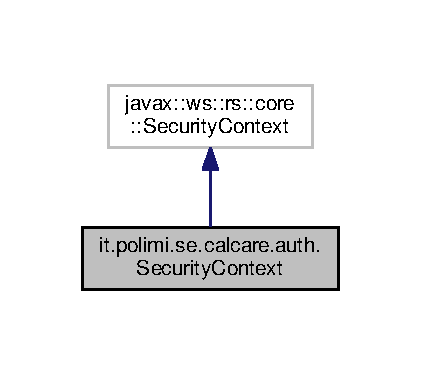
\includegraphics[width=202pt]{classit_1_1polimi_1_1se_1_1calcare_1_1auth_1_1SecurityContext__inherit__graph}
\end{center}
\end{figure}


Collaboration diagram for it.\+polimi.\+se.\+calcare.\+auth.\+Security\+Context\+:
\nopagebreak
\begin{figure}[H]
\begin{center}
\leavevmode
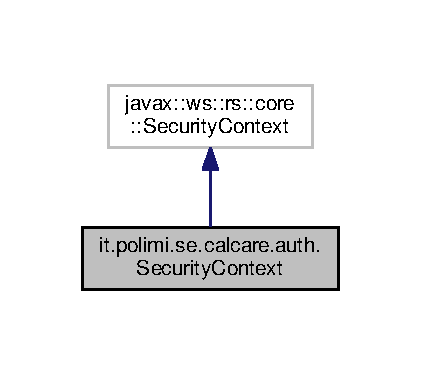
\includegraphics[width=202pt]{classit_1_1polimi_1_1se_1_1calcare_1_1auth_1_1SecurityContext__coll__graph}
\end{center}
\end{figure}
\subsection*{Public Member Functions}
\begin{DoxyCompactItemize}
\item 
\hypertarget{classit_1_1polimi_1_1se_1_1calcare_1_1auth_1_1SecurityContext_ac550381ff255793aac3080ec0f4b8935}{}{\bfseries Security\+Context} (\hyperlink{classit_1_1polimi_1_1se_1_1calcare_1_1entities_1_1User}{User} user)\label{classit_1_1polimi_1_1se_1_1calcare_1_1auth_1_1SecurityContext_ac550381ff255793aac3080ec0f4b8935}

\item 
\hypertarget{classit_1_1polimi_1_1se_1_1calcare_1_1auth_1_1SecurityContext_a8db291c84bb2972b8b5bd115fe745f25}{}Principal {\bfseries get\+User\+Principal} ()\label{classit_1_1polimi_1_1se_1_1calcare_1_1auth_1_1SecurityContext_a8db291c84bb2972b8b5bd115fe745f25}

\item 
\hypertarget{classit_1_1polimi_1_1se_1_1calcare_1_1auth_1_1SecurityContext_a20e2a14403001d4b81974326ccfc02e7}{}boolean {\bfseries is\+User\+In\+Role} (String role)\label{classit_1_1polimi_1_1se_1_1calcare_1_1auth_1_1SecurityContext_a20e2a14403001d4b81974326ccfc02e7}

\item 
\hypertarget{classit_1_1polimi_1_1se_1_1calcare_1_1auth_1_1SecurityContext_aae76dfe134788a1f72e85a15bf9d2dd0}{}boolean {\bfseries is\+Secure} ()\label{classit_1_1polimi_1_1se_1_1calcare_1_1auth_1_1SecurityContext_aae76dfe134788a1f72e85a15bf9d2dd0}

\item 
\hypertarget{classit_1_1polimi_1_1se_1_1calcare_1_1auth_1_1SecurityContext_a6008e031210ed2b659f42e1b0a5ee7e0}{}String {\bfseries get\+Authentication\+Scheme} ()\label{classit_1_1polimi_1_1se_1_1calcare_1_1auth_1_1SecurityContext_a6008e031210ed2b659f42e1b0a5ee7e0}

\end{DoxyCompactItemize}


\subsection{Detailed Description}
\begin{DoxyAuthor}{Author}
tyrion 
\end{DoxyAuthor}


The documentation for this class was generated from the following file\+:\begin{DoxyCompactItemize}
\item 
src/main/java/it/polimi/se/calcare/auth/Security\+Context.\+java\end{DoxyCompactItemize}

\hypertarget{classit_1_1polimi_1_1se_1_1calcare_1_1helpers_1_1SendMail}{}\section{it.\+polimi.\+se.\+calcare.\+helpers.\+Send\+Mail Class Reference}
\label{classit_1_1polimi_1_1se_1_1calcare_1_1helpers_1_1SendMail}\index{it.\+polimi.\+se.\+calcare.\+helpers.\+Send\+Mail@{it.\+polimi.\+se.\+calcare.\+helpers.\+Send\+Mail}}
\subsection*{Static Public Member Functions}
\begin{DoxyCompactItemize}
\item 
\hypertarget{classit_1_1polimi_1_1se_1_1calcare_1_1helpers_1_1SendMail_af802832f1339614a60df99dbfaf70728}{}static void {\bfseries Mail} (String\mbox{[}$\,$\mbox{]} to, String subject, String body)\label{classit_1_1polimi_1_1se_1_1calcare_1_1helpers_1_1SendMail_af802832f1339614a60df99dbfaf70728}

\end{DoxyCompactItemize}


The documentation for this class was generated from the following file\+:\begin{DoxyCompactItemize}
\item 
src/main/java/it/polimi/se/calcare/helpers/Send\+Mail.\+java\end{DoxyCompactItemize}

\hypertarget{classit_1_1polimi_1_1se_1_1calcare_1_1entities_1_1User}{}\section{it.\+polimi.\+se.\+calcare.\+entities.\+User Class Reference}
\label{classit_1_1polimi_1_1se_1_1calcare_1_1entities_1_1User}\index{it.\+polimi.\+se.\+calcare.\+entities.\+User@{it.\+polimi.\+se.\+calcare.\+entities.\+User}}


Inheritance diagram for it.\+polimi.\+se.\+calcare.\+entities.\+User\+:
\nopagebreak
\begin{figure}[H]
\begin{center}
\leavevmode
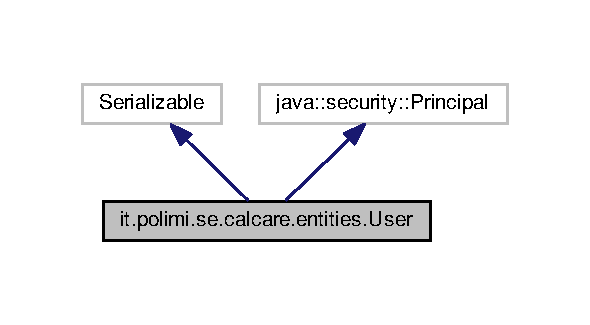
\includegraphics[width=283pt]{classit_1_1polimi_1_1se_1_1calcare_1_1entities_1_1User__inherit__graph}
\end{center}
\end{figure}


Collaboration diagram for it.\+polimi.\+se.\+calcare.\+entities.\+User\+:
\nopagebreak
\begin{figure}[H]
\begin{center}
\leavevmode
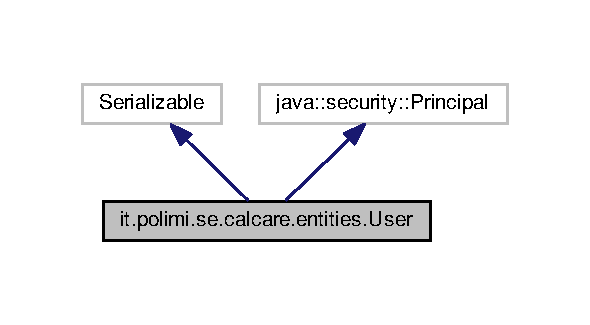
\includegraphics[width=283pt]{classit_1_1polimi_1_1se_1_1calcare_1_1entities_1_1User__coll__graph}
\end{center}
\end{figure}
\subsection*{Public Member Functions}
\begin{DoxyCompactItemize}
\item 
\hypertarget{classit_1_1polimi_1_1se_1_1calcare_1_1entities_1_1User_ace8d24a3ab5be15665186d7c8889582e}{}{\bfseries User} (Integer id)\label{classit_1_1polimi_1_1se_1_1calcare_1_1entities_1_1User_ace8d24a3ab5be15665186d7c8889582e}

\item 
\hypertarget{classit_1_1polimi_1_1se_1_1calcare_1_1entities_1_1User_acb37891090b4c06cc25a49046efc3dbe}{}{\bfseries User} (String email, String password)\label{classit_1_1polimi_1_1se_1_1calcare_1_1entities_1_1User_acb37891090b4c06cc25a49046efc3dbe}

\item 
\hypertarget{classit_1_1polimi_1_1se_1_1calcare_1_1entities_1_1User_a1c33c54067a0934f8fc09df29b48a37b}{}{\bfseries User} (String email, String password, String given\+Name, String family\+Name)\label{classit_1_1polimi_1_1se_1_1calcare_1_1entities_1_1User_a1c33c54067a0934f8fc09df29b48a37b}

\item 
\hypertarget{classit_1_1polimi_1_1se_1_1calcare_1_1entities_1_1User_a79b8ea82511aa84c11cceb9edc7b6153}{}Integer {\bfseries get\+Id} ()\label{classit_1_1polimi_1_1se_1_1calcare_1_1entities_1_1User_a79b8ea82511aa84c11cceb9edc7b6153}

\item 
\hypertarget{classit_1_1polimi_1_1se_1_1calcare_1_1entities_1_1User_a45e369dbbe0c91fda1942845cee6b641}{}void {\bfseries set\+Id} (Integer id)\label{classit_1_1polimi_1_1se_1_1calcare_1_1entities_1_1User_a45e369dbbe0c91fda1942845cee6b641}

\item 
\hypertarget{classit_1_1polimi_1_1se_1_1calcare_1_1entities_1_1User_a0876b563f776a37ad18e0e6849edfd62}{}String {\bfseries get\+Email} ()\label{classit_1_1polimi_1_1se_1_1calcare_1_1entities_1_1User_a0876b563f776a37ad18e0e6849edfd62}

\item 
\hypertarget{classit_1_1polimi_1_1se_1_1calcare_1_1entities_1_1User_a2eafc265554e1224fc1d87ac2ddf935e}{}void {\bfseries set\+Email} (String email)\label{classit_1_1polimi_1_1se_1_1calcare_1_1entities_1_1User_a2eafc265554e1224fc1d87ac2ddf935e}

\item 
\hypertarget{classit_1_1polimi_1_1se_1_1calcare_1_1entities_1_1User_af62ba7d1cadd8a5c5b3aa360ea804942}{}String {\bfseries get\+Password} ()\label{classit_1_1polimi_1_1se_1_1calcare_1_1entities_1_1User_af62ba7d1cadd8a5c5b3aa360ea804942}

\item 
\hypertarget{classit_1_1polimi_1_1se_1_1calcare_1_1entities_1_1User_afca81a9b6a45d4553311ada249f47a25}{}void {\bfseries set\+Password} (String password)  throws No\+Such\+Algorithm\+Exception, Invalid\+Key\+Spec\+Exception \label{classit_1_1polimi_1_1se_1_1calcare_1_1entities_1_1User_afca81a9b6a45d4553311ada249f47a25}

\item 
\hypertarget{classit_1_1polimi_1_1se_1_1calcare_1_1entities_1_1User_a54e0f0d6a87b4aee121a61550b4c2402}{}String {\bfseries get\+Given\+Name} ()\label{classit_1_1polimi_1_1se_1_1calcare_1_1entities_1_1User_a54e0f0d6a87b4aee121a61550b4c2402}

\item 
\hypertarget{classit_1_1polimi_1_1se_1_1calcare_1_1entities_1_1User_a1ffa1bbf99911a6fc16072b31054eb41}{}void {\bfseries set\+Given\+Name} (String given\+Name)\label{classit_1_1polimi_1_1se_1_1calcare_1_1entities_1_1User_a1ffa1bbf99911a6fc16072b31054eb41}

\item 
\hypertarget{classit_1_1polimi_1_1se_1_1calcare_1_1entities_1_1User_a606f2b3ccd41ac6dabc0aae2c13d1a30}{}String {\bfseries get\+Family\+Name} ()\label{classit_1_1polimi_1_1se_1_1calcare_1_1entities_1_1User_a606f2b3ccd41ac6dabc0aae2c13d1a30}

\item 
\hypertarget{classit_1_1polimi_1_1se_1_1calcare_1_1entities_1_1User_a931b2b94c6b3c3d9e939e1abb05fbbd0}{}void {\bfseries set\+Family\+Name} (String family\+Name)\label{classit_1_1polimi_1_1se_1_1calcare_1_1entities_1_1User_a931b2b94c6b3c3d9e939e1abb05fbbd0}

\item 
\hypertarget{classit_1_1polimi_1_1se_1_1calcare_1_1entities_1_1User_a8a580bed776f7123015da79f4c6d9a3c}{}String {\bfseries get\+Full\+Name} ()\label{classit_1_1polimi_1_1se_1_1calcare_1_1entities_1_1User_a8a580bed776f7123015da79f4c6d9a3c}

\item 
\hypertarget{classit_1_1polimi_1_1se_1_1calcare_1_1entities_1_1User_abaf43f595f1a95e4d5249004eb4a2baa}{}boolean {\bfseries is\+Active} ()\label{classit_1_1polimi_1_1se_1_1calcare_1_1entities_1_1User_abaf43f595f1a95e4d5249004eb4a2baa}

\item 
\hypertarget{classit_1_1polimi_1_1se_1_1calcare_1_1entities_1_1User_afb673a8a8fd5f065f433df18a173c360}{}void {\bfseries set\+Active} (boolean active)\label{classit_1_1polimi_1_1se_1_1calcare_1_1entities_1_1User_afb673a8a8fd5f065f433df18a173c360}

\item 
\hypertarget{classit_1_1polimi_1_1se_1_1calcare_1_1entities_1_1User_aa921aadc0d7f429e1ac75cceeccb4108}{}\hyperlink{classit_1_1polimi_1_1se_1_1calcare_1_1entities_1_1Calendar}{Calendar} {\bfseries get\+Calendar} ()\label{classit_1_1polimi_1_1se_1_1calcare_1_1entities_1_1User_aa921aadc0d7f429e1ac75cceeccb4108}

\item 
\hypertarget{classit_1_1polimi_1_1se_1_1calcare_1_1entities_1_1User_a12962da9b1c479b7f32843c11489d2cc}{}void {\bfseries set\+Calendar} (\hyperlink{classit_1_1polimi_1_1se_1_1calcare_1_1entities_1_1Calendar}{Calendar} calendar)\label{classit_1_1polimi_1_1se_1_1calcare_1_1entities_1_1User_a12962da9b1c479b7f32843c11489d2cc}

\item 
\hypertarget{classit_1_1polimi_1_1se_1_1calcare_1_1entities_1_1User_afda09cd9c7cbf34438340f58f43989e5}{}Collection$<$ \hyperlink{classit_1_1polimi_1_1se_1_1calcare_1_1entities_1_1Event}{Event} $>$ {\bfseries get\+Event\+Collection} ()\label{classit_1_1polimi_1_1se_1_1calcare_1_1entities_1_1User_afda09cd9c7cbf34438340f58f43989e5}

\item 
\hypertarget{classit_1_1polimi_1_1se_1_1calcare_1_1entities_1_1User_a0ccf3d9e2adeacb34fb7860c4e6eadaf}{}void {\bfseries set\+Event\+Collection} (Collection$<$ \hyperlink{classit_1_1polimi_1_1se_1_1calcare_1_1entities_1_1Event}{Event} $>$ event\+Collection)\label{classit_1_1polimi_1_1se_1_1calcare_1_1entities_1_1User_a0ccf3d9e2adeacb34fb7860c4e6eadaf}

\item 
\hypertarget{classit_1_1polimi_1_1se_1_1calcare_1_1entities_1_1User_adc20fc9b44d9b5aa2027e08372be768b}{}Collection$<$ \hyperlink{classit_1_1polimi_1_1se_1_1calcare_1_1entities_1_1Notification}{Notification} $>$ {\bfseries get\+Notification\+Collection} ()\label{classit_1_1polimi_1_1se_1_1calcare_1_1entities_1_1User_adc20fc9b44d9b5aa2027e08372be768b}

\item 
\hypertarget{classit_1_1polimi_1_1se_1_1calcare_1_1entities_1_1User_ae911fc5b99e2e592ce84a7113fd5e272}{}void {\bfseries set\+Notification\+Collection} (Collection$<$ \hyperlink{classit_1_1polimi_1_1se_1_1calcare_1_1entities_1_1Notification}{Notification} $>$ notification\+Collection)\label{classit_1_1polimi_1_1se_1_1calcare_1_1entities_1_1User_ae911fc5b99e2e592ce84a7113fd5e272}

\item 
\hypertarget{classit_1_1polimi_1_1se_1_1calcare_1_1entities_1_1User_acb2b12f16e293c2f752138d8dc47435c}{}int {\bfseries hash\+Code} ()\label{classit_1_1polimi_1_1se_1_1calcare_1_1entities_1_1User_acb2b12f16e293c2f752138d8dc47435c}

\item 
\hypertarget{classit_1_1polimi_1_1se_1_1calcare_1_1entities_1_1User_a8603c798e9a1003f0a2b0c436446ca1d}{}boolean {\bfseries equals} (Object object)\label{classit_1_1polimi_1_1se_1_1calcare_1_1entities_1_1User_a8603c798e9a1003f0a2b0c436446ca1d}

\item 
\hypertarget{classit_1_1polimi_1_1se_1_1calcare_1_1entities_1_1User_a1f6bafd14868c6f966c4c1dacafbeb8c}{}String {\bfseries to\+String} ()\label{classit_1_1polimi_1_1se_1_1calcare_1_1entities_1_1User_a1f6bafd14868c6f966c4c1dacafbeb8c}

\item 
\hypertarget{classit_1_1polimi_1_1se_1_1calcare_1_1entities_1_1User_a8287e3bc4d33047219c300b0a9fd6cc2}{}String {\bfseries get\+Name} ()\label{classit_1_1polimi_1_1se_1_1calcare_1_1entities_1_1User_a8287e3bc4d33047219c300b0a9fd6cc2}

\end{DoxyCompactItemize}


\subsection{Detailed Description}
\begin{DoxyAuthor}{Author}
tyrion 
\end{DoxyAuthor}


The documentation for this class was generated from the following file\+:\begin{DoxyCompactItemize}
\item 
src/main/java/it/polimi/se/calcare/entities/User.\+java\end{DoxyCompactItemize}

\hypertarget{classit_1_1polimi_1_1se_1_1calcare_1_1service_1_1UserFacadeREST}{}\section{it.\+polimi.\+se.\+calcare.\+service.\+User\+Facade\+R\+E\+S\+T Class Reference}
\label{classit_1_1polimi_1_1se_1_1calcare_1_1service_1_1UserFacadeREST}\index{it.\+polimi.\+se.\+calcare.\+service.\+User\+Facade\+R\+E\+S\+T@{it.\+polimi.\+se.\+calcare.\+service.\+User\+Facade\+R\+E\+S\+T}}


Inheritance diagram for it.\+polimi.\+se.\+calcare.\+service.\+User\+Facade\+R\+E\+S\+T\+:
\nopagebreak
\begin{figure}[H]
\begin{center}
\leavevmode
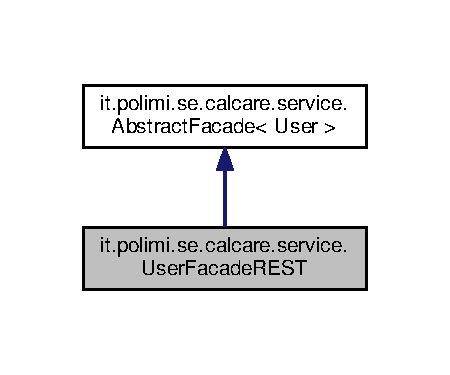
\includegraphics[width=216pt]{classit_1_1polimi_1_1se_1_1calcare_1_1service_1_1UserFacadeREST__inherit__graph}
\end{center}
\end{figure}


Collaboration diagram for it.\+polimi.\+se.\+calcare.\+service.\+User\+Facade\+R\+E\+S\+T\+:
\nopagebreak
\begin{figure}[H]
\begin{center}
\leavevmode
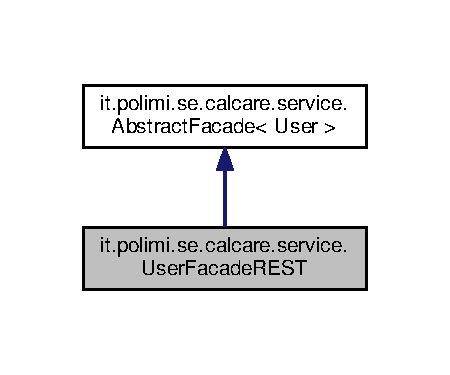
\includegraphics[width=216pt]{classit_1_1polimi_1_1se_1_1calcare_1_1service_1_1UserFacadeREST__coll__graph}
\end{center}
\end{figure}
\subsection*{Public Member Functions}
\begin{DoxyCompactItemize}
\item 
\hypertarget{classit_1_1polimi_1_1se_1_1calcare_1_1service_1_1UserFacadeREST_aaca56f16be182c6dbd6f9b58efbfc21a}{}Response {\bfseries add} (@Context Uri\+Info ui, \hyperlink{classit_1_1polimi_1_1se_1_1calcare_1_1entities_1_1User}{User} entity)  throws No\+Such\+Algorithm\+Exception, Invalid\+Key\+Spec\+Exception \label{classit_1_1polimi_1_1se_1_1calcare_1_1service_1_1UserFacadeREST_aaca56f16be182c6dbd6f9b58efbfc21a}

\item 
\hypertarget{classit_1_1polimi_1_1se_1_1calcare_1_1service_1_1UserFacadeREST_adecf3d47f4dbf8b92656b7b113f0b0a5}{}void {\bfseries edit} (@Context Security\+Context sc, \hyperlink{classit_1_1polimi_1_1se_1_1calcare_1_1entities_1_1User}{User} entity)\label{classit_1_1polimi_1_1se_1_1calcare_1_1service_1_1UserFacadeREST_adecf3d47f4dbf8b92656b7b113f0b0a5}

\item 
\hypertarget{classit_1_1polimi_1_1se_1_1calcare_1_1service_1_1UserFacadeREST_a14a274c408505ea91f938878535a78b7}{}void {\bfseries remove} (@Context Security\+Context sc)\label{classit_1_1polimi_1_1se_1_1calcare_1_1service_1_1UserFacadeREST_a14a274c408505ea91f938878535a78b7}

\item 
\hypertarget{classit_1_1polimi_1_1se_1_1calcare_1_1service_1_1UserFacadeREST_a3e931230f45796f19dd0daffb0ffb8b4}{}\hyperlink{classit_1_1polimi_1_1se_1_1calcare_1_1entities_1_1User}{User} {\bfseries get} (@Context Security\+Context sc)\label{classit_1_1polimi_1_1se_1_1calcare_1_1service_1_1UserFacadeREST_a3e931230f45796f19dd0daffb0ffb8b4}

\item 
\hypertarget{classit_1_1polimi_1_1se_1_1calcare_1_1service_1_1UserFacadeREST_aeee94d2e3cfeb5041d8026fca0675d4d}{}List$<$ \hyperlink{classit_1_1polimi_1_1se_1_1calcare_1_1entities_1_1User}{User} $>$ {\bfseries find\+All} ()\label{classit_1_1polimi_1_1se_1_1calcare_1_1service_1_1UserFacadeREST_aeee94d2e3cfeb5041d8026fca0675d4d}

\end{DoxyCompactItemize}
\subsection*{Protected Member Functions}
\begin{DoxyCompactItemize}
\item 
\hypertarget{classit_1_1polimi_1_1se_1_1calcare_1_1service_1_1UserFacadeREST_a111911bc228956ba9f3bf4bca11b349b}{}Entity\+Manager {\bfseries get\+Entity\+Manager} ()\label{classit_1_1polimi_1_1se_1_1calcare_1_1service_1_1UserFacadeREST_a111911bc228956ba9f3bf4bca11b349b}

\end{DoxyCompactItemize}


\subsection{Detailed Description}
\begin{DoxyAuthor}{Author}
tyrion 
\end{DoxyAuthor}


The documentation for this class was generated from the following file\+:\begin{DoxyCompactItemize}
\item 
src/main/java/it/polimi/se/calcare/service/User\+Facade\+R\+E\+S\+T.\+java\end{DoxyCompactItemize}

\hypertarget{classit_1_1polimi_1_1se_1_1calcare_1_1entities_1_1WeatherCondition}{}\section{it.\+polimi.\+se.\+calcare.\+entities.\+Weather\+Condition Class Reference}
\label{classit_1_1polimi_1_1se_1_1calcare_1_1entities_1_1WeatherCondition}\index{it.\+polimi.\+se.\+calcare.\+entities.\+Weather\+Condition@{it.\+polimi.\+se.\+calcare.\+entities.\+Weather\+Condition}}


Inheritance diagram for it.\+polimi.\+se.\+calcare.\+entities.\+Weather\+Condition\+:
\nopagebreak
\begin{figure}[H]
\begin{center}
\leavevmode
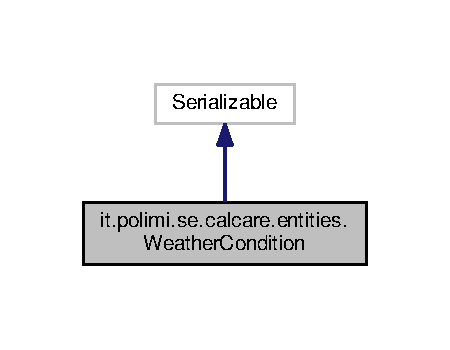
\includegraphics[width=216pt]{classit_1_1polimi_1_1se_1_1calcare_1_1entities_1_1WeatherCondition__inherit__graph}
\end{center}
\end{figure}


Collaboration diagram for it.\+polimi.\+se.\+calcare.\+entities.\+Weather\+Condition\+:
\nopagebreak
\begin{figure}[H]
\begin{center}
\leavevmode
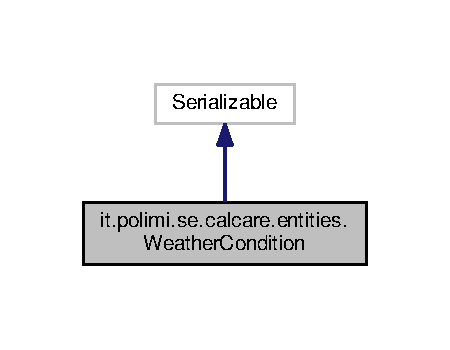
\includegraphics[width=216pt]{classit_1_1polimi_1_1se_1_1calcare_1_1entities_1_1WeatherCondition__coll__graph}
\end{center}
\end{figure}
\subsection*{Public Member Functions}
\begin{DoxyCompactItemize}
\item 
\hypertarget{classit_1_1polimi_1_1se_1_1calcare_1_1entities_1_1WeatherCondition_a00c0cd171da722b3ad7c585705fa4e95}{}{\bfseries Weather\+Condition} (Integer id)\label{classit_1_1polimi_1_1se_1_1calcare_1_1entities_1_1WeatherCondition_a00c0cd171da722b3ad7c585705fa4e95}

\item 
\hypertarget{classit_1_1polimi_1_1se_1_1calcare_1_1entities_1_1WeatherCondition_a6db94d45467b640b16941f53cea5c4d7}{}{\bfseries Weather\+Condition} (Integer id, String name, String description, String icon)\label{classit_1_1polimi_1_1se_1_1calcare_1_1entities_1_1WeatherCondition_a6db94d45467b640b16941f53cea5c4d7}

\item 
\hypertarget{classit_1_1polimi_1_1se_1_1calcare_1_1entities_1_1WeatherCondition_a0435cf83fe43e4c1f91dc3c4a67372f0}{}Integer {\bfseries get\+Id} ()\label{classit_1_1polimi_1_1se_1_1calcare_1_1entities_1_1WeatherCondition_a0435cf83fe43e4c1f91dc3c4a67372f0}

\item 
\hypertarget{classit_1_1polimi_1_1se_1_1calcare_1_1entities_1_1WeatherCondition_ada713c8b3183d7dbc784c65137cc134e}{}void {\bfseries set\+Id} (Integer id)\label{classit_1_1polimi_1_1se_1_1calcare_1_1entities_1_1WeatherCondition_ada713c8b3183d7dbc784c65137cc134e}

\item 
\hypertarget{classit_1_1polimi_1_1se_1_1calcare_1_1entities_1_1WeatherCondition_a36a94e78f944d906c209d2496f36f3b3}{}String {\bfseries get\+Name} ()\label{classit_1_1polimi_1_1se_1_1calcare_1_1entities_1_1WeatherCondition_a36a94e78f944d906c209d2496f36f3b3}

\item 
\hypertarget{classit_1_1polimi_1_1se_1_1calcare_1_1entities_1_1WeatherCondition_a0f72cbdc034995e9f3d49f51c7481cfd}{}void {\bfseries set\+Name} (String name)\label{classit_1_1polimi_1_1se_1_1calcare_1_1entities_1_1WeatherCondition_a0f72cbdc034995e9f3d49f51c7481cfd}

\item 
\hypertarget{classit_1_1polimi_1_1se_1_1calcare_1_1entities_1_1WeatherCondition_afdd95174d07504c843bb04fbc58babd5}{}String {\bfseries get\+Description} ()\label{classit_1_1polimi_1_1se_1_1calcare_1_1entities_1_1WeatherCondition_afdd95174d07504c843bb04fbc58babd5}

\item 
\hypertarget{classit_1_1polimi_1_1se_1_1calcare_1_1entities_1_1WeatherCondition_a857fa008a9f13c5f423520469976ab4a}{}void {\bfseries set\+Description} (String description)\label{classit_1_1polimi_1_1se_1_1calcare_1_1entities_1_1WeatherCondition_a857fa008a9f13c5f423520469976ab4a}

\item 
\hypertarget{classit_1_1polimi_1_1se_1_1calcare_1_1entities_1_1WeatherCondition_a0b5248c9fa248809e6a6487f71656d75}{}String {\bfseries get\+Icon} ()\label{classit_1_1polimi_1_1se_1_1calcare_1_1entities_1_1WeatherCondition_a0b5248c9fa248809e6a6487f71656d75}

\item 
\hypertarget{classit_1_1polimi_1_1se_1_1calcare_1_1entities_1_1WeatherCondition_a74ddfcb08d6757ef6203a9dfe2c38b97}{}void {\bfseries set\+Icon} (String icon)\label{classit_1_1polimi_1_1se_1_1calcare_1_1entities_1_1WeatherCondition_a74ddfcb08d6757ef6203a9dfe2c38b97}

\item 
\hypertarget{classit_1_1polimi_1_1se_1_1calcare_1_1entities_1_1WeatherCondition_ad6822dfbce9197d2bb8b2c3a6c3dd95b}{}Collection$<$ \hyperlink{classit_1_1polimi_1_1se_1_1calcare_1_1entities_1_1Forecast}{Forecast} $>$ {\bfseries get\+Forecast\+Collection} ()\label{classit_1_1polimi_1_1se_1_1calcare_1_1entities_1_1WeatherCondition_ad6822dfbce9197d2bb8b2c3a6c3dd95b}

\item 
\hypertarget{classit_1_1polimi_1_1se_1_1calcare_1_1entities_1_1WeatherCondition_a3672929152fa52e16d87f8f5c4892b71}{}void {\bfseries set\+Forecast\+Collection} (Collection$<$ \hyperlink{classit_1_1polimi_1_1se_1_1calcare_1_1entities_1_1Forecast}{Forecast} $>$ forecast\+Collection)\label{classit_1_1polimi_1_1se_1_1calcare_1_1entities_1_1WeatherCondition_a3672929152fa52e16d87f8f5c4892b71}

\item 
\hypertarget{classit_1_1polimi_1_1se_1_1calcare_1_1entities_1_1WeatherCondition_aca4e31ef321843c6245129c712e9cd98}{}int {\bfseries hash\+Code} ()\label{classit_1_1polimi_1_1se_1_1calcare_1_1entities_1_1WeatherCondition_aca4e31ef321843c6245129c712e9cd98}

\item 
\hypertarget{classit_1_1polimi_1_1se_1_1calcare_1_1entities_1_1WeatherCondition_a92a10b5697f4da18002db6aabeace184}{}boolean {\bfseries equals} (Object object)\label{classit_1_1polimi_1_1se_1_1calcare_1_1entities_1_1WeatherCondition_a92a10b5697f4da18002db6aabeace184}

\item 
\hypertarget{classit_1_1polimi_1_1se_1_1calcare_1_1entities_1_1WeatherCondition_abbfc382d672b67356d4cfd1b845c53d7}{}String {\bfseries to\+String} ()\label{classit_1_1polimi_1_1se_1_1calcare_1_1entities_1_1WeatherCondition_abbfc382d672b67356d4cfd1b845c53d7}

\end{DoxyCompactItemize}


\subsection{Detailed Description}
\begin{DoxyAuthor}{Author}
tyrion 
\end{DoxyAuthor}


The documentation for this class was generated from the following file\+:\begin{DoxyCompactItemize}
\item 
src/main/java/it/polimi/se/calcare/entities/Weather\+Condition.\+java\end{DoxyCompactItemize}

\hypertarget{classit_1_1polimi_1_1se_1_1calcare_1_1service_1_1WeatherConditionFacadeREST}{}\section{it.\+polimi.\+se.\+calcare.\+service.\+Weather\+Condition\+Facade\+R\+E\+S\+T Class Reference}
\label{classit_1_1polimi_1_1se_1_1calcare_1_1service_1_1WeatherConditionFacadeREST}\index{it.\+polimi.\+se.\+calcare.\+service.\+Weather\+Condition\+Facade\+R\+E\+S\+T@{it.\+polimi.\+se.\+calcare.\+service.\+Weather\+Condition\+Facade\+R\+E\+S\+T}}


Inheritance diagram for it.\+polimi.\+se.\+calcare.\+service.\+Weather\+Condition\+Facade\+R\+E\+S\+T\+:
\nopagebreak
\begin{figure}[H]
\begin{center}
\leavevmode
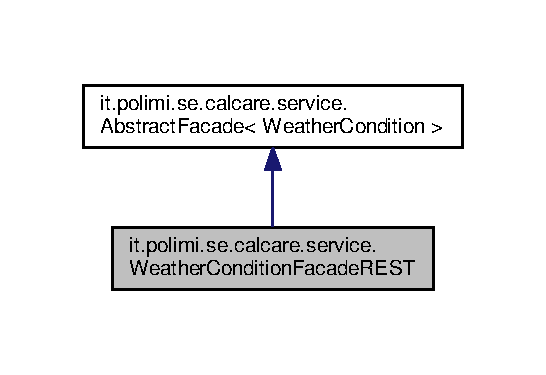
\includegraphics[width=262pt]{classit_1_1polimi_1_1se_1_1calcare_1_1service_1_1WeatherConditionFacadeREST__inherit__graph}
\end{center}
\end{figure}


Collaboration diagram for it.\+polimi.\+se.\+calcare.\+service.\+Weather\+Condition\+Facade\+R\+E\+S\+T\+:
\nopagebreak
\begin{figure}[H]
\begin{center}
\leavevmode
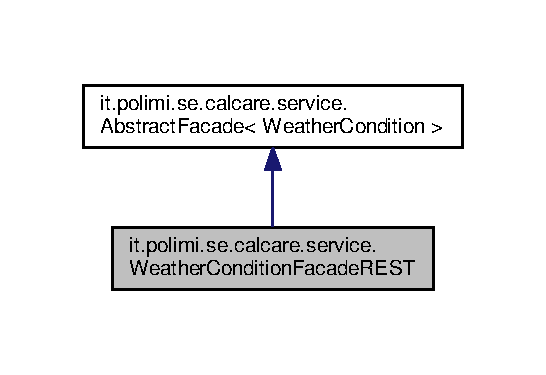
\includegraphics[width=262pt]{classit_1_1polimi_1_1se_1_1calcare_1_1service_1_1WeatherConditionFacadeREST__coll__graph}
\end{center}
\end{figure}
\subsection*{Public Member Functions}
\begin{DoxyCompactItemize}
\item 
\hypertarget{classit_1_1polimi_1_1se_1_1calcare_1_1service_1_1WeatherConditionFacadeREST_af0d9cd15745526ae62d3165c829a76f3}{}void {\bfseries create} (\hyperlink{classit_1_1polimi_1_1se_1_1calcare_1_1entities_1_1WeatherCondition}{Weather\+Condition} entity)\label{classit_1_1polimi_1_1se_1_1calcare_1_1service_1_1WeatherConditionFacadeREST_af0d9cd15745526ae62d3165c829a76f3}

\item 
\hypertarget{classit_1_1polimi_1_1se_1_1calcare_1_1service_1_1WeatherConditionFacadeREST_ae77c199121809cb4f981c9c46853c5aa}{}void {\bfseries edit} (@Path\+Param(\char`\"{}id\char`\"{}) Integer id, \hyperlink{classit_1_1polimi_1_1se_1_1calcare_1_1entities_1_1WeatherCondition}{Weather\+Condition} entity)\label{classit_1_1polimi_1_1se_1_1calcare_1_1service_1_1WeatherConditionFacadeREST_ae77c199121809cb4f981c9c46853c5aa}

\item 
\hypertarget{classit_1_1polimi_1_1se_1_1calcare_1_1service_1_1WeatherConditionFacadeREST_a3be687743b6864da4a0d715c9beccb53}{}void {\bfseries remove} (@Path\+Param(\char`\"{}id\char`\"{}) Integer id)\label{classit_1_1polimi_1_1se_1_1calcare_1_1service_1_1WeatherConditionFacadeREST_a3be687743b6864da4a0d715c9beccb53}

\item 
\hypertarget{classit_1_1polimi_1_1se_1_1calcare_1_1service_1_1WeatherConditionFacadeREST_a9c0770d623bfbac387e33253d98a9774}{}\hyperlink{classit_1_1polimi_1_1se_1_1calcare_1_1entities_1_1WeatherCondition}{Weather\+Condition} {\bfseries find} (@Path\+Param(\char`\"{}id\char`\"{}) Integer id)\label{classit_1_1polimi_1_1se_1_1calcare_1_1service_1_1WeatherConditionFacadeREST_a9c0770d623bfbac387e33253d98a9774}

\item 
\hypertarget{classit_1_1polimi_1_1se_1_1calcare_1_1service_1_1WeatherConditionFacadeREST_a3240296d145a16d0fe156787b9813661}{}List$<$ \hyperlink{classit_1_1polimi_1_1se_1_1calcare_1_1entities_1_1WeatherCondition}{Weather\+Condition} $>$ {\bfseries find\+All} ()\label{classit_1_1polimi_1_1se_1_1calcare_1_1service_1_1WeatherConditionFacadeREST_a3240296d145a16d0fe156787b9813661}

\item 
\hypertarget{classit_1_1polimi_1_1se_1_1calcare_1_1service_1_1WeatherConditionFacadeREST_a68f643443b9a89e89d459c4539c9fb10}{}List$<$ \hyperlink{classit_1_1polimi_1_1se_1_1calcare_1_1entities_1_1WeatherCondition}{Weather\+Condition} $>$ {\bfseries find\+Range} (@Path\+Param(\char`\"{}from\char`\"{}) Integer from,@Path\+Param(\char`\"{}to\char`\"{}) Integer to)\label{classit_1_1polimi_1_1se_1_1calcare_1_1service_1_1WeatherConditionFacadeREST_a68f643443b9a89e89d459c4539c9fb10}

\item 
\hypertarget{classit_1_1polimi_1_1se_1_1calcare_1_1service_1_1WeatherConditionFacadeREST_a6bb840c228acac6e2967d6818e4d154a}{}String {\bfseries count\+R\+E\+S\+T} ()\label{classit_1_1polimi_1_1se_1_1calcare_1_1service_1_1WeatherConditionFacadeREST_a6bb840c228acac6e2967d6818e4d154a}

\end{DoxyCompactItemize}
\subsection*{Protected Member Functions}
\begin{DoxyCompactItemize}
\item 
\hypertarget{classit_1_1polimi_1_1se_1_1calcare_1_1service_1_1WeatherConditionFacadeREST_a3f662ba0d4eac5eb7698e0662abd0095}{}Entity\+Manager {\bfseries get\+Entity\+Manager} ()\label{classit_1_1polimi_1_1se_1_1calcare_1_1service_1_1WeatherConditionFacadeREST_a3f662ba0d4eac5eb7698e0662abd0095}

\end{DoxyCompactItemize}


\subsection{Detailed Description}
\begin{DoxyAuthor}{Author}
tyrion 
\end{DoxyAuthor}


The documentation for this class was generated from the following file\+:\begin{DoxyCompactItemize}
\item 
src/main/java/it/polimi/se/calcare/service/Weather\+Condition\+Facade\+R\+E\+S\+T.\+java\end{DoxyCompactItemize}

%--- End generated contents ---

% Index
\backmatter
\newpage
\phantomsection
\clearemptydoublepage
\addcontentsline{toc}{chapter}{Index}
\printindex

\end{document}
